\documentclass[a4paper,11pt,fleqn,dvipsnames,twoside,openright,sort&compress]{memoir} 	% Openright aabner kapitler paa hoejresider (openany begge)

%%%% PACKAGES %%%%

% ¤¤ Oversaettelse og tegnsaetning ¤¤ %
\usepackage[utf8]{inputenc}					% Input-indkodning af tegnsaet (UTF8)
\usepackage[british, danish]{babel}					% Dokumentets sprog
\usepackage[T1]{fontenc}					% Output-indkodning af tegnsaet (T1)
\usepackage{ragged2e,anyfontsize}			% Justering af elementer
\usepackage{nomencl}
\makenomenclature
\usepackage{indentfirst}

% ¤¤ Figurer og tabeller (floats) ¤¤ %
% Tilføjet:
\usepackage{tabularx}
\usepackage{longtable}
\usepackage{graphicx}
\usepackage{pdfpages}
%Linjeskift i tabeller:
\newcommand{\specialcell}[2][c]{%
  \begin{tabular}[#1]{@{}c@{}}#2\end{tabular}}

  %anvend: \specialcell[]{Første del\\ anden del} [t]= align top, [b]= align bottom


% Tyk horisontallinje til tabeller :
\makeatletter
\newcommand{\thickhline}{%
    \noalign {\ifnum 0=`}\fi \hrule height 1.5pt
    \futurelet \reserved@a \@xhline
}
\newcolumntype{"}{@{\hskip\tabcolsep\vrule width 2pt\hskip\tabcolsep}}
\makeatother

% Anvend : \thickhline

\usepackage{tabulary}
\usepackage{graphicx} 						% Haandtering af eksterne billeder (JPG, PNG, EPS, PDF)
\usepackage{wrapfig}
%\usepackage{eso-pic}						% Tilfoej billedekommandoer paa hver side
%\usepackage{wrapfig}						% Indsaettelse af figurer omsvoebt af tekst. \begin{wrapfigure}{Placering}{Stoerrelse}
\usepackage{multirow}                		% Fletning af raekker og kolonner (\multicolumn og \multirow)
\usepackage{multicol}         	        	% Muliggoer output i spalter
\usepackage{rotating}						% Rotation af tekst med \begin{sideways}...\end{sideways}
\usepackage{colortbl} 						% Farver i tabeller (fx \columncolor og \rowcolor)
\usepackage{xcolor}							% Definer farver med \definecolor. Se mere: http://en.wikibooks.org/wiki/LaTeX/Colors
\usepackage{flafter}						% Soerger for at floats ikke optraeder i teksten foer deres reference
\let\newfloat\relax 						% Justering mellem float-pakken og memoir
\usepackage{float}							% Muliggoer eksakt placering af floats, f.eks. \begin{figure}[H]

\graphicspath{{billeder/}}						% Sti til figure

% ¤¤ Matematik mm. ¤¤
\usepackage{amsmath,amssymb,stmaryrd} 		% Avancerede matematik-udvidelser
\usepackage{mathtools}						% Andre matematik- og tegnudvidelser
\usepackage{textcomp}                 		% Symbol-udvidelser (f.eks. promille-tegn med \textperthousand )
\usepackage{amsthm}
\usepackage{rsphrase}						% Kemi-pakke til RS-saetninger, f.eks. \rsphrase{R1}
\usepackage[version=3]{mhchem} 				% Kemi-pakke til flot og let notation af formler, f.eks. \ce{Fe2O3}
\usepackage[binary-units=true, per-mode=fraction]{siunitx}						% Flot og konsistent
\DeclareSIUnit\vote{stemme}
\DeclareSIUnit\votes{stemmer}
%\SI{tal}{enhed}
\sisetup{output-decimal-marker = {,}}		% Opsaetning af \SI (DE for komma som decimalseparator)
\usepackage{icomma}							% Komma som decimal operator

% ¤¤ Referencer og kilder ¤¤ %
\usepackage[danish, english]{varioref}				% Muliggoer bl.a. krydshenvisninger med sidetal (\vref)
\usepackage[numbers]{natbib}							% Udvidelse med naturvidenskabelige citationsmodeller
%\usepackage{xr}							% Referencer til eksternt dokument med \externaldocument{<NAVN>}
%\usepackage{glossaries}					% Terminologi- eller symbolliste (se mere i Daleifs Latex-bog)
% ¤¤ Misc. ¤¤ %
\usepackage{listings}						% Placer kildekode i dokumentet med \begin{lstlisting}...\end{lstlisting}
\usepackage{lipsum}							% Dummy text \lipsum[..]
\usepackage[shortlabels]{enumitem}			% Muliggoer enkelt konfiguration af lister
\usepackage{pdfpages}
\usepackage{pdflscape}					% Goer det muligt at inkludere pdf-dokumenter med kommandoen \includepdf[pages={x-y}]{fil.pdf}
\pdfoptionpdfminorversion=6					% Muliggoer inkludering af pdf dokumenter, af version 1.6 og hoejere
\pretolerance=2500 							% Justering af afstand mellem ord (hoejt tal, mindre orddeling og mere luft mellem ord)

% Kommentarer og rettelser med \fxnote. Med 'final' i stedet for 'draft' udloeser hver note en error i den faerdige rapport.
\usepackage{footnote}
\usepackage[footnote,draft,danish,silent,nomargin]{fixme}
\makesavenoteenv{tabular}


\usepackage[ntheorem]{mdframed} %Bruges for at kunne lave definitionsboksene

\usepackage{filecontents}

%%%% CUSTOM SETTINGS %%%%
%%%%To-do markater%%%%
\usepackage{todonotes}

%%Tikz%%
\usepackage{tikz}
\usepackage{tikz-uml}
\usetikzlibrary{shapes.geometric, arrows, chains, matrix, mindmap, patterns, shapes.misc, trees, positioning}

%rettet fra Emilie%
\tikzstyle{startstop} = [rectangle, ultra thick, rounded corners, minimum width=3cm, minimum height=1cm,text centered, text width=3cm, draw=black, fill=white]
\tikzstyle{io} = [trapezium, trapezium left angle=80, trapezium right angle=80, ultra thick, minimum width=3cm, minimum height=1cm, text centered, draw=black, fill=white]
\tikzstyle{process} = [rectangle, thick, minimum width=1cm, minimum height=0.75cm, text centered, draw=black, fill=white]
\tikzstyle{simple} = [rectangle, minimum width=1cm, minimum height=0.75cm, text centered, fill=white]
\tikzstyle{specialprocess} = [rectangle, ultra thick, minimum width=3cm, minimum height=1cm, text centered, draw=black, fill=white]
\tikzstyle{decision} = [diamond, ultra thick, minimum width=3cm, minimum height=1cm, text centered, draw=black, fill=white]
\tikzstyle{seconddecision} = [circle, ultra thick, minimum width=3cm, minimum height=1cm, text centered, draw=black, fill=white]
\tikzstyle{predefined} = [rectangle, rounded corners, ultra thick, minimum width=3cm, minimum height=1cm,text centered, text width=3cm, draw=black, fill=white]
\tikzstyle{data} = [trapezium, trapezium left angle=60, trapezium right angle=120, ultra thick, minimum width=3cm, minimum height=1cm, text centered, draw=black, fill=white]
\tikzstyle{terminator} = [ellipse, ultra thick, minimum width=3cm, minimum height=1cm, text centered, draw=black, fill=white]
\tikzstyle{arrow} = [->,>=open triangle 90]

\tikzstyle{decision} = [diamond, draw, fill=blue!20,
    text width=4.5em, text badly centered, node distance=3cm, inner sep=0pt]
\tikzstyle{block} = [rectangle, draw, fill=blue!20,
    text width=5em, text centered, rounded corners, minimum height=4em]
\tikzstyle{line} = [draw, -latex']
\tikzstyle{cloud} = [draw, ellipse,fill=red!20, node distance=3cm,
    minimum height=2em]

%PGF%
\usepackage{pgfplots}
\usepgfplotslibrary{patchplots}

%%Boxes%%
\definecolor{theoline}{gray}{0.5}
\definecolor{theocolor}{gray}{0.9}
\definecolor{lemcolor}{gray}{0.97}
\definecolor{defcolor}{RGB}{214,234,218}

\mdfdefinestyle{box}{ % saving some space
skipabove=1.5em plus 0.4em minus 0.6em,
%skipbelow=0.5em plus 0.4em minus 0.2em,
%leftmargin=-7pt, rightmargin=-7pt,
innerleftmargin=3pt,innerrightmargin=7pt, innertopmargin=2pt, innerbottommargin=2pt,
%linewidth=1pt,
%splittopskip=3.2em minus 0.2em,
%splitbottomskip=0.5em plus 0.2em minus 0.1em,
}
\newmdtheoremenv[style=box,linecolor=theoline,backgroundcolor=theocolor]{theorem}{Theorem}[section]
\newmdtheoremenv[style=box,linecolor=theoline,backgroundcolor=lemcolor]{lemma}[theorem]{Lemma}
\newmdtheoremenv[style=box,linecolor=theoline,backgroundcolor=lemcolor]{proposition}[theorem]{Proposition}
\newmdtheoremenv[style=box,linecolor=theoline,backgroundcolor=lemcolor]{corollary}[theorem]{Corollary}



%\newtheorem{theorem}{Theorem}[section]
%\newtheorem{lemma}[theorem]{Lemma}
%\newtheorem{proposition}[theorem]{Proposition}
%\newtheorem{corollary}[theorem]{Corollary}
%\newtheorem{case}{Bevis}[theorem]
%\newtheorem{defn}{Definition}[section]

\renewenvironment{proof}[1][Proof]{\begin{trivlist}
\item[\hskip \labelsep {\bfseries #1}]}{\end{trivlist}}

\newenvironment{definition}[1][Definition]{\begin{trivlist}
\item[\hskip \labelsep {\bfseries #1}]}{\end{trivlist}}

\newenvironment{remark}[1][Remark]{\begin{trivlist}
\item[\hskip \labelsep {\bfseries #1}]}{\end{trivlist}}



\theoremstyle{definition}
\newmdtheoremenv[style=box,linecolor=theoline,backgroundcolor=lemcolor]{defn}[theorem]{Definition}

\newtheorem{eks}[theorem]{Example}
\surroundwithmdframed[
   topline=false,
   rightline=false,
   bottomline=false,
   leftmargin=\parindent,
   skipabove=\medskipamount,
   skipbelow=\medskipamount
]{eks}

\newenvironment{example}[1][Example]{\begin{trivlist}
\item[\hskip \labelsep {\bfseries #1}]}{\end{trivlist}}
\surroundwithmdframed[
   topline=false,
   rightline=false,
   bottomline=false,
   leftmargin=\parindent,
   skipabove=\medskipamount,
   skipbelow=\medskipamount
]{example}

\renewcommand{\qed}{\nobreak \ifvmode \relax \else
      \ifdim\lastskip<1.5em \hskip-\lastskip
      \hskip1.5em plus0em minus0.5em \fi \nobreak
      \vrule height0.75em width0.5em depth0.25em\fi}

% ¤¤ Marginer ¤¤ %
\setlrmarginsandblock{3.5cm}{2.5cm}{*}		% \setlrmarginsandblock{Indbinding}{Kant}{Ratio}
\setulmarginsandblock{2.5cm}{3.0cm}{*}		% \setulmarginsandblock{Top}{Bund}{Ratio}
\checkandfixthelayout 						% Oversaetter vaerdier til brug for andre pakker

%	¤¤ Afsnitsformatering ¤¤ %
\setlength{\parindent}{3mm}           		% Stoerrelse af indryk
\setlength{\parskip}{3mm}          			% Afstand mellem afsnit ved brug af double Enter
\linespread{1,1}							% Linie afstand

% ¤¤ Litteraturlisten ¤¤ %
%\bibpunct[,]{[}{]}{;}{a}{,}{,} 				% Definerer de 6 parametre ved Harvard henvisning (bl.a. parantestype og seperatortegn)
\bibliographystyle{unsrtnat}			% Udseende af litteraturlisten.

% ¤¤ Indholdsfortegnelse ¤¤ %
\setsecnumdepth{subsubsection}		 			% Dybden af nummerede overkrifter (part/chapter/section/subsection)
\maxsecnumdepth{subsubsection}					% Dokumentklassens graense for nummereringsdybde
\settocdepth{subsection} 					% Dybden af indholdsfortegnelsen

% ¤¤ Lister ¤¤ %
\setlist{
  topsep=0pt,								% Vertikal afstand mellem tekst og listen
  itemsep=-1ex,								% Vertikal afstand mellem items
}

% ¤¤ Visuelle referencer ¤¤ %
\usepackage[colorlinks,
            pdftex,
            pdfauthor={Andreas Madsen, Anja Nielsen, Anna Bonde, Astrid Ipsen, Henrik Christensen, Rasmus Kjær og Taniya Henriksen},
            pdftitle={Fanciful Handbook Management},
            pdfsubject={Developing a Handbook Management System for SMBs},
            pdfkeywords={handbooks,document,compsci},
            pdfproducer={Latex with hyperref},
            pdfcreator={pdflatex, or other tool}]{hyperref}			% Danner klikbare referencer (hyperlinks) i dokumentet.
\hypersetup{colorlinks = true,				% Opsaetning af farvede hyperlinks (interne links, citeringer og URL)
    linkcolor = black,
    citecolor = black,
    urlcolor = black
}

% ¤¤ Opsaetning af - og tabeltekst ¤¤ %
\captionnamefont{\small\bfseries\itshape}	% Opsaetning af tekstdelen ('Figur' eller 'Tabel')
\captiontitlefont{\small}					% Opsaetning af nummerering
\captiondelim{. }							% Seperator mellem nummerering og figurtekst
\hangcaption								% Venstrejusterer flere-liniers figurtekst under hinanden
\captionwidth{\linewidth}					% Bredden af figurteksten
\setlength{\belowcaptionskip}{0pt}			% Afstand under figurteksten
\addto\captionsdanish{\renewcommand{\figurename}{Figure}} %Aendre figurteksten til dansk

% ¤¤ Opsaetning af listings ¤¤ %

\definecolor{commentGreen}{RGB}{34,139,24}
\definecolor{stringPurple}{RGB}{208,76,239}


\lstset{language=[Sharp]C,					% Sprog
	basicstyle=\fontsize{11}{13}\selectfont\ttfamily,		% Opsaetning af teksten
	keywords={for,if,while,else,elseif,		% Noegleord at fremhaeve
			  end,break,return,case,
			  switch,function},
	keywordstyle=\color{blue},				% Opsaetning af noegleord
	commentstyle=\color{commentGreen},		% Opsaetning af kommentarer
	stringstyle=\color{stringPurple},		% Opsaetning af strenge
	showstringspaces=false,					% Mellemrum i strenge enten vist eller blanke
	numbers=left, numberstyle=\tiny,		% Linjenumre
	extendedchars=true, 					% Tillader specielle karakterer
	columns=flexible,						% Kolonnejustering
	breaklines, breakatwhitespace=true,		% Bryd lange linjer
	frame=single,
	morekeywords = {
	public,
	static,
	string,
	bool,
	int,
	void}
}

\lstMakeShortInline[columns=fixed]|
\lstset{language=C,captionpos=b}

% ¤¤ Navngivning ¤¤ %
\addto\captionsdanish{
	\renewcommand\appendixname{Appendix}
	\renewcommand\contentsname{Contents}
	\renewcommand\bibname{Bibliography}
	\renewcommand\appendixpagename{Appendix}
	\renewcommand\appendixtocname{Appendix}
	%\renewcommand\cftchaptername{Kapitel~}
%\renewcommand\cftchaptername{\chaptername~}
% Skriver "Kapitel" foran kapitlerne i indholdsfortegnelsen
	\renewcommand\cftappendixname{Appendix ~}
	%\renewcommand\cftappendixname{\appendixname~}			% Skriver "Appendiks" foran appendiks i indholdsfortegnelsen
}

% ¤¤ Kapiteludssende ¤¤ %
\definecolor{numbercolor}{RGB}{130,0,50}
	% Definerer en farve til brug til kapiteludseende
\newif\ifchapternonum

\makechapterstyle{jenor}{					% Definerer kapiteludseende frem til ...
  \renewcommand\beforechapskip{0pt}
  \renewcommand\printchaptername{}
  \renewcommand\printchapternum{}
  \renewcommand\printchapternonum{\chapternonumtrue}
  \renewcommand\chaptitlefont{\fontfamily{pbk}\fontseries{db}\fontshape{n}\fontsize{25}{35}\selectfont\raggedleft}
  \renewcommand\chapnumfont{\fontfamily{pbk}\fontseries{m}\fontshape{n}\fontsize{1in}{0in}\selectfont\color{numbercolor}}
  \renewcommand\printchaptertitle[1]{%
    \noindent
    \ifchapternonum
    \begin{tabularx}{\textwidth}{X}
    {\let\\\newline\chaptitlefont ##1\par}
    \end{tabularx}
    \par\vskip-2.5mm\hrule
    \else
    \begin{tabularx}{\textwidth}{Xl}
    {\parbox[b]{\linewidth}{\chaptitlefont ##1}} & \raisebox{-15pt}{\chapnumfont \thechapter}
    \end{tabularx}
    \par\vskip2mm\hrule
    \fi
  }
}											% ... her

\chapterstyle{jenor}						% Valg af kapiteludseende - Google 'memoir chapter styles' for alternativer

% ¤¤ Sidehoved ¤¤ %

\makepagestyle{AAU}							% Definerer sidehoved og sidefod udseende frem til ...
\makepsmarks{AAU}{%
	\createmark{chapter}{left}{shownumber}{}{. \ }
	\createmark{section}{right}{shownumber}{}{. \ }
	\createplainmark{toc}{both}{\contentsname}
	\createplainmark{lof}{both}{\listfigurename}
	\createplainmark{lot}{both}{\listtablename}
	\createplainmark{bib}{both}{\bibname}
	\createplainmark{index}{both}{\indexname}
	\createplainmark{glossary}{both}{\glossaryname}
}
\nouppercaseheads											% Ingen Caps oenskes

\makeevenhead{AAU}{Gruppe: DAT2 B2-2}{}{\leftmark}				% Definerer lige siders sidehoved (\makeevenhead{Navn}{Venstre}{Center}{Hoejre})
\makeoddhead{AAU}{\rightmark}{}{Aalborg Universitet}		% Definerer ulige siders sidehoved (\makeoddhead{Navn}{Venstre}{Center}{Hoejre})
\makeevenfoot{AAU}{\thepage}{}{}							% Definerer lige siders sidefod (\makeevenfoot{Navn}{Venstre}{Center}{Hoejre})
\makeoddfoot{AAU}{}{}{\thepage}								% Definerer ulige siders sidefod (\makeoddfoot{Navn}{Venstre}{Center}{Hoejre})
\makeheadrule{AAU}{\textwidth}{0.5pt}						% Tilfoejer en streg under sidehovedets indhold
\makefootrule{AAU}{\textwidth}{0.5pt}{1mm}					% Tilfoejer en streg under sidefodens indhold

\copypagestyle{AAUchap}{AAU}								% Sidehoved for kapitelsider defineres som standardsider, men med blank sidehoved
\makeoddhead{AAUchap}{}{}{}
\makeevenhead{AAUchap}{}{}{}
\makeheadrule{AAUchap}{\textwidth}{0pt}
\aliaspagestyle{chapter}{AAUchap}							% Den ny style vaelges til at gaelde for chapters
															% ... her

\pagestyle{AAU}												% Valg af sidehoved og sidefod


%%%% CUSTOM COMMANDS %%%%

% ¤¤ Billede hack ¤¤ %
\newcommand{\figur}[4]{
		\begin{figure}[H] \centering
			\includegraphics[width=#1\textwidth]{billeder/#2}
			\caption{#3}\label{#4}
		\end{figure}
}

% ¤¤ Specielle tegn ¤¤ %
\newcommand{\decC}{^{\circ}\text{C}}
\newcommand{\dec}{^{\circ}}
\newcommand{\m}{\cdot}


%%%% ORDDELING %%%%

\hyphenation{}

%Mads
\usepackage[strings]{underscore}
%\usepackage{nccmath}
%\usepackage{breqn}
\usepackage{amsmath}
\usepackage{cleveref}
\usepackage{epigraph}

\crefname{table}{table}{tables}
\Crefname{table}{Tables}{Tables}
\crefname{figure}{figure}{figures}
\Crefname{figure}{Figure}{Figures}
\crefname{equation}{equation}{equations}
\Crefname{equation}{Equation}{Equations}
\crefname{section}{section}{sections}
\Crefname{section}{Section}{Sections}
\crefname{subsection}{section}{sections}
\Crefname{subsection}{Section}{Sections}
\crefname{subsubsection}{section}{sections}
\Crefname{subsubsection}{Section}{Sections}
\crefname{chapter}{chapter}{chapters}
\Crefname{chapter}{Chapter}{Chapters}
\crefname{appendix}{appendix}{appendixes}
\Crefname{appendix}{Appendix}{Appendixes}
\crefname{eks}{example}{examples}
\Crefname{eks}{Example}{Examples}
\crefname{theorem}{theorem}{theorems}
\Crefname{theorem}{Theorem}{Theorems}
\crefname{defn}{definition}{definitions}
\Crefname{defn}{Definition}{Definitions}
\crefname{lstlisting}{listing}{listings}
\Crefname{lstlisting}{Listing}{Listings}




\newcommand{\SubItem}[1]{
	{\setlength\itemindent{15pt} \item[-] #1}
}

 %Preamble indlaeses

\raggedbottom %Sørger for at LaTeX ikke "strækker" teksten

\begin{document}

\frontmatter




\thispagestyle{empty}
\begin{flushright}

\vspace{3cm}

\phantom{hul}

\phantom{hul}

\phantom{hul}

\textsl{\Huge  OB-Handbooks} \\ \vspace{1cm}

\rule{13cm}{3mm} \\ \vspace{1.5cm}
\vspace{1cm}

\vspace{2cm} 
\textsc{\Large P3 project - Development of applications\\
Gruppe ds304e19 \\
Computer Science \& Software Engineering\\
Aalborg University\\
19/12/19\\}
\end{flushright}

\cleardoublepage

% Dette er LaTeX-versionen af titelbladet for TNB studenterrapporter
% Filen kræver:
% Universitetets logo:  AAU-logo-stud-UK eller AAU-logo-stud-DK
% Synopsis: En fil ved navn synopsis.tex

% Udarbejdet af: Jesper Nørgaard (jesper@noergaard.eu) 10. april 2012

\phantomsection
\pdfbookmark[0]{English title page}{label:titlepage_en}
\thispagestyle{empty}

\begin{minipage}[t]{0.48\textwidth}
\vspace*{-25pt}			%\vspace*{-9pt}

\includegraphics[height=4cm]{billeder/AAU-logo-stud-UK-RGB.pdf}
\end{minipage}
\hfill
\begin{minipage}[t]{0.48\textwidth}
{\small 
\textbf{Third Semester}\\
\textbf{Electronics and IT}  \\
Selma lagerløfs Vej 300 \\
Aalborg University \\
9220 Aalborg \\
%http://www.tnb.aau.dk
}
\end{minipage}

\vspace*{1cm}

\begin{minipage}[t]{0.48\textwidth}
\textbf{Project Title:} \\[5pt]\hspace*{2ex}
Development of Applications

\textbf{Scientific Theme:} \\[5pt]\hspace{2ex}
Document management\\
for handbooks

\textbf{Project Period:} \\[5pt]\bigskip\hspace{2ex}
Fall Semester 2019

\textbf{Project Group:} \\[5pt]\bigskip\hspace{2ex}
ds304e19

\textbf{Project group:} \\[5pt]\hspace*{2ex}
Andreas Leicht Madsen \\\hspace*{2ex}
Anja Elisasen Lumholtz Nielsen \\\hspace*{2ex}
Anna Veibel Bonde \\\hspace*{2ex}
Astrid Ipsen \\\hspace*{2ex}
Henrik Abel Christensen \\\hspace*{2ex}
Rasmus Rendal Kjær \\\hspace*{2ex}
Taniya Rianthong Henriksen \\\hspace*{2ex}

\textbf{Supervisor:} \\[5pt]\hspace*{2ex}
Lu Chen \\\hspace*{2ex}

\vspace*{1cm}

%\textbf{Oplagstal: ?} \\
\textbf{Page Number Total: \color{red}{???}}\\
\textbf{Page Number Main: \pageref{LastPage} }\\
\textbf{Appendix: \color{red}{???}} \\ 
\textbf{Completion Date: 19/12-2019}

\end{minipage}
\hfill
\begin{minipage}[t]{0.483\textwidth}
\textbf{Abstract:} \\[5pt]
\fbox{\parbox{8cm}{\bigskipDenne rapport er baseret på et systemudviklingsprojekt stillet af Pia Ipsen. 
Udviklingsprojektet går ud på at designe og udvikle et billigt dokumentstyringssystem til håndtering af en håndbog og eventuelle dokumenter der bruges i forbindelse med godkendelse af leverandører.\\

Rapporten beskriver udviklingen af systemet OBHandbooks, samt de forskellige analyser og proccessor anvendt.
Systemet er udviklet og designet iterativt hovedssageligt på baggrund af objekt orienteret analyse og design metoder.\\

Fokusset for udviklingen har været at lave et system som understøtter delproblemet: håndteringen af en håndbog og dets dokumenter.
\\
Gennem en række interviews og usability test er systemets funktionaliteter og det generelle design blevet afklaret.
Resultatet er en systemdefinition, kravs specifikation, samt andre analyse elementer, som lagde grundlaget for systemet OBHandbooks.
Dette system har de grundlæggende nødvendige funktionaliteter for det stillede projekt, men før det kan tages i brug er der brug for at rette op på nogen bugs, såsom markeringen af om en bruger har læst nødvendige dokumenter i håndbogen.
Desuden, vil de enkelte UI's skulle finpudses før systemet kan tages i brug.

\bigskip}}
\end{minipage}

\vfill

{\footnotesize\itshape The content of the report is freely available, but publication (with source reference) may only take place in agreement with the authors.}

%Rapportens indhold er frit tilgængeligt, men offentliggørelse (med kildeangivelse) må kun ske efter aftale med forfatterne.
% The content of the report is freely available, but publication (with source reference) may only take place in agreement with the authors.
\cleardoublepage

% FORORD MED LÆSEVEJLEDNING %
\chapter*{Preface\markboth{Preface}{Preface}}\label{ch:preface}
This development project is undertaken by the project group ds304e19 during the third semester computer science and software engineering at Aalborg University, autumn 2019.
The headline of the project period was "\textit{Application development - from user to data, algorithms and test - and back again}

\noindent \textbf{Reading Guide}\\
References to sources is done in accordance with the Vancouver method, where a source is represented with a number X in between $[\ ]$, e.g. $[17]$ is a reference to source number 17 in the bibliography. 
\\\indent
References inside the study is done by giving a type and a number, e.g listing number three in chapter six is noted as listing 6.3.
\\\indent
Additionally, a number of concepts and names are abbreviated throughout the report.
A list of these abbreviations can be found in \cref{sec:abbrivitation}.




% Underskrifter %

\phantom{Luft}

\textit{Group ds304e19 - Computer Science \& Software Engineering - Aalborg University}

\phantom{Luft}

\phantom{Luft}

\begin{table}[H]
	\centering
		\begin{tabular}{c c c}
			\underline{\phantom{mmmmmmmmmmmmmmmm}} & \underline{\phantom{mmmmmmmmmmmmmmmm}} & \underline{\phantom{mmmmmmmmmmmmmmmm}} \\
			Andreas leicht Madsen & Anja Elisasen Lumholtz Nielsen 				& Anna Veibel Bonde	\\
			&&\\
			&&\\
			\end{tabular}
			\begin{tabular}{c c c}
			\centering			
			  \underline{\phantom{mmmmmmmmmmmmmmmm}} & \underline{\phantom{mmmmmmmmmmmmmmmm}} & \underline{\phantom{mmmmmmmmmmmmmmmm}} \\
			Astrid Ipsen & Henrik Abel Christensen & Rasmus Rendal Kjær\\
			&&\\
			&&\\               						
		\end{tabular}
	\begin{tabular}{c c c}
		\centering			
%		\underline{\phantom{mmmmmmmmmmmmmmmm}}
		\qquad \qquad \qquad  &\underline{\phantom{mmmmmmmmmmmmmmmm}} & \\ 
%		  \underline{\phantom{mmmmmmmmmmmmmmmm}} \\
		 & Taniya Rianthong Henriksen & \\
		&&\\
		&&\\               						
	\end{tabular}
\end{table}
\cleardoublepage

%%%% Indholdsfortegnelse (TOC) %%%%

%\phantomsection

\pdfbookmark[0]{Indholdsfortegnelse}{indhold}

\tableofcontents*

%\listoftodos

\mainmatter


\chapter{Introduction}
\section{Initial problem statement}
\section{Work method}
The strategy is selected according to the principles presented in the OOA\&D method. This method puts great emphasis post-poning non-critical decisions so as to maintain the freedom to make changes once more information is available and on working on the areas that pose the greatest challenge first. %Anja: Præsenter OOA&D metoden før du nævner den.

% I don't understand the next sentence here
% Taniya: does the set of questions have a name?
A set of questions supposed to serve as a starting point for determining which area that is, is provided in the book [howdidwedothisagain]. The questions are answered so that a yes equals to zero points, a maybe to one point and a no to two points. If the answer is unknown it is counted as a no. The more points an area has the more critical the corresponding area is. The list of these questions and answers can be found in appendix XX.
% Henrik: Synes ikke der burde var BLANK linie her, da de to afsnit hænger sammen
Based on this activity it was concluded that AAA is the most difficult area, with BBB as number two and CCC last.
% Maybe a sort of chapter division here?
% Anja: Generelt skal den ovenstående tekst stå et andet sted. Informationen virker lidt malplaceret.
Selection of a general work structure depends on the degrees of structure and complexity in the project. The waterfall model, where one part of the project is completely finished before the next one is begun is great for projects with low uncertainty and high complexity. However an iterative approach where every part of the project is revisited  multiple times is better for projects with high uncertainty and low complexity. [how does one refer to things the teacher has said but which are not in his own damned book?] % I think you have to find a book that says it

The user is someone who works with handbooks in a professional setting and therefore either has or quickly gains a lot of experience. The task is very structured and one of the main purposes of the system is to make sure that the books remain structured in the face of human errors. The developers on the project however are students with limited experience, which is what provides the most uncertainty to this project. %Anja: Jeg synes ikke, at vi skal skrive, at grunden til at, der er "uncertainty" i projektet pga., at vi er studerende. Det er mere fordi at selve designprocessen i sig selv er usikker/omskiftelig. Hele grundlaget for at have en 'design'-proces til at starte med er, at vi ikke ved hvordan slutproduktet skal se ud på forhånd; derfor er projektet "uncertain".
% Henrik: Hvad er det "the developers" har limited experience med?

The size of the project can be adjusted until it fits the length of the project period and the amount of users is relatively low: There is only one main user and a few who are not as involved. The amount of the new information is very high at the beginning of the project but once understood the complexity is insignificant.

As both the uncertainty and complexity of the project are relatively low, both methods can be used. As there is a high complexity in the very beginning of the project the waterfall method will be used here with an iterative process in the remaining parts of the project to make sure the terms were not misunderstood and to deliver the best possible system to the users. %Nævn gerne noget med designprocessen her.
%Anja: Ellers er teksten fin (y)
% Henrik: Måske flyt dette afsnit op sammen med det tidligere afsnit, hvor der snakkes om "unvertainty and complexity"?

\todo[inline]{Vi skal måske have snakket om placeringen af denne tekst igen. Jeg synes, at den kommer lidt malplaceret ift. indledning. Jeg synes, at det giver mere mening efter problemanalysen.}


\subsection{Iterative design process}
The benefit of working with iteratively is to continually talk with the users and discuss their needs and wants, determine or redetermine requirements. and design a system which gets refined along the way. This ongoing communication with the users and their needs is likewise the center of user-centered approach where there’s a focus on the user’s tasks, empirical measurement and iterative design. (Sharp, Rogers \& Preece)

There are four basic activities when working interaction design which are; \textit{establishing requirements, designing alternatives, prototyping,} and \textit{evaluating}. To be able to design a system with the user’s needs and wants in mind it is imperative to know the target users and which activities the system needs to support. This is done through establishing requirements where information of the target users is gathered through data gathering and analysis. When the requirements are settled it is possible to design alternatives where ideas a suggested that meet these requirements. Here a conceptual design is formed which describes an abstract outline of how the users can interact with it. Concrete designs infers to the details of the design; which could include colors, sounds, images etc. (Sharp, Rogers \& Preece)

When the design alternative phase is complete a prototype can be developed. The purpose of the prototype is to evaluate with the users whether the criteria has been met and give them an idea of how the system could potentially turn out. The prototype doesn’t necessarily have to consist of a working piece of software; the prototype could also be paper-based in the early stages of the design process. When the prototype is complete then it can be measured an evaluated. The evaluation phase determines whether or not the design is usable and/or acceptable. (Sharp, Rogers \& Preece)

\subsubsection{A simple lifecycle model}
All of the before-mentioned activities are related in an iterative design process. This is shown visually in figure xx. The lifecycle model is a simplified version of reality and isn’t meant to be prescriptive, and depending on the project it isn’t always possible to go through all of the phases described. Though the model is developed through Sharp, Rogers and Preece’s research of how software engineering is practiced in the field. (Sharp, Rogers \& Preece)

According to Sharp, Rogers and Preece “Most projects start with establishing requirements” (p. 333). It is from this first activity that it’s possible to go into the ‘designing alternatives’ activity from where a prototype. in the ‘prototyping’ activity, can be developed which in turn can be evaluated by the users in the ‘evaluating’ activity. From this evaluation the designers can specify new or redefined requirements, or they can go directly to redesign or deem the project done.

\subsubsection{Using of the lifecycle model in the project}
Throughout the project it is intended to design a system iteratively with a specific user’s needs and wants integrated into the designs and tests. This is the basis of choosing to work with the lifecycle model as a model to reflect over which activity is being used throughout the stages of the project. The lifecycle model is likewise a good indicator of when an iteration is done and when a new one has been commenced. 

As mentioned by Sharp, Rogers and Preece most projects starts with establishing requirements, which will be reflected in this project with an initial interview where the first requirements will be determined. This is intended to result in a following design process and prototype which can be evaluated with the user in a second interview.
\chapter{Preliminary case analysis}
In the following chapter the case and related information will be presented.
To gather information about the case, and its underlying problems, interviews have been held with the project's stakeholder, Pia Ipsen, who will henceforth be referred to as Ipsen.
During the course of this project Ipsen was interviewed five times:
Three times to mainly gain information on the problem and application domain where one was to clarify a few questions about the problem domain, and twice in relation to larger usability testing of the implemented system.

The information gained from these interviews is used in this chapter to briefly present the case in \cref{sec:CaseDescription}.
The chapter will additionally present standards and their relation to the case in \cref{sec:standards}.
Furthermore, existing solutions will discussed in \cref{sec:existingsolutionsintro}.
Based upon this, the system definition is presented in \cref{sec:SystemDefinition}.
Finally, the chapter will end in a problem statement which guides the scope of the project.

The knowledge gained from the interviews will be further analyzed in \cref{ch:ProblemDomain} and \cref{ch:ApplicationDomain}.

\section{Case description} \label{sec:CaseDescription}

This report will be based on the case presented by Ipsen, who is a senior consultant for the firm QMS-Consult.
This firm guides companies on how to maintain or write handbooks, to follow given standards, such that the companies can acquire or keep their certifications.
In her work she helps the companies with their handbooks and in a few cases acts as the company's quality manager.
The case presented in this report is made from the viewpoint of her acting as a quality manager for a small firm rather than as a consultant.
All information in this section is based upon interviews with her.

A handbook consist of several documents that each describe procedures or guidelines for different aspects of a firm and its workings.
There exists several versions of each document where only the newest version is active, and all of the previous versions are required to be archived for at least three to five years. All of these documents must adhere to a set of rules, notably the following:

\begin{itemize}
	\item
	A document must always be up-to-date.
	In reality it is sometimes only a yearly review.
	\item
	When a new version is written it must be approved by usually one or two people before it is added to the handbook.
	\item
	Each document has a title with an ID that can only be associated with that specific title.
	Such that when a title has been paired with an ID, the ID can no longer be associated with any other titles, even if the current title should be deleted.
\end{itemize}

Additionally, as a service to the readers, Ipsen will highlight changes in between versions.
This is a service, not a requirement.
However in some standards it is a requirement to submit a changelog detailing the reason for the changes made.

While the documents are only required to be archived for three to five years in reality previous versions are seldomly ever deleted.
This is due to the hassle of determining files that are no longer needed and due to the relatively small space required to store them.

Ipsen works together with the firms to make sure that their handbooks are in good shape for audit.
The secretaries have the responsibility of managing the handbook documents and the everyday workers who work at the firm.
Whenever a new document has been updated it is imperative that the workers read and understand the documents relevant to them and do so immediately.
Not all documents are relevant for every worker, as the daily responsibilities of the workers can vary.

The problem with the current work procedure is that all the documents are stored in folders on a computer and Ipsen manually keeps track of older documents as well as the active ones.
This manual work method takes time and has a high risk of mistakes:
It can be complicated to keep track of the newest documents and their approval stages.

Ipsen requires a system that can manage the documents and their versions.
The system should furthermore be used to ensure that the everyday workers have read the relevant documents.

A more in depth analysis of Ipsens case will be explored in the FACTOR-analysis in \cref{sec:factorcriteria} and the rich picture analysis in \cref{sec:richpictures}.

There exists specific standards for how to maintain these handbooks.
These will be elaborated in the next section.

\section{Standards}
% Rasmus - I think that it is also important to mention how standards play a role of ensuring trust between organisations, in that it can help ensure that everyone is doing stuff properly. Also, auditing is probably a process that should be mentioned, as that is part of standards workflow
A standard is in its core an agreed way of doing things. This is a broad term that applies to production, management, quality and most activities are done by organizations. So, the point of standards is to cover a wide variety of topics and give workers a basis for the expectation of their work. An organization might use a \textit{Quality Management Standard} (QMS) to help efficiency and quality of production or use a Food Standard to keep the food from being rotten or more so to keep the quality of the food at level.

If we for example look at the building of a house, then there could be a technical standard that says that a house has a foundation, four walls and a roof. Then another quality standard could say that the foundation should be made of cement as it has a more long-term lifespan. More so there could be a safety standard that says that walls are not allowed to be built higher than a certain height because of the danger of collapsing. These are all simple examples of standards, but organizations like the \textit{International Standard Organization} (ISO) has 22811 standards that organizations can apply in different situations.
\subsection{ISO 9001}
% Rasmus - This doesn't seem super concrete, and more like a sales speech for ISO. In the problem analysis, we should probably focus on what parts of ISO are essential to our project specifically.
The ISO 9001 is a QMS that gives, if complied with, a certification showing customers that the organization have been checked by a special auditor. These auditors are not from ISO themselves but from a certified third party.
This QMS is based on 7 Quality Management Principles(QMP):

\begin{enumerate}
        \item Customer focus: Is used to set requirements for customer service and thereby increase quality of service.
        \item Leadership: This QMP focuses on unity in the work and creating conditions that make people achieve the organization's quality objectives.
        \item Engagement of people: Giving people of all levels in the organization motivation to enhance quality of work.
        \item Process approach: Getting consistent results by increasing the quality of the working process.
        \item Improvement: Successful organizations keep focusing on the improvement of the organization.
        \item Evidence-based decision making: Making decisions based on gathered data and information.
        \item Relationship management: An organization manages relationships with suppliers or similar people to gain sustained success.
\end{enumerate}

These principles are used in the ISO 9001 to set the criteria for quality,
quality principles are broad which makes the ISO 9001 usable in many different areas of work.
The gained certification is not permanent, but needs to be renewed every few years.
\newline
Kilde: https://www.iso.org/iso-9001-quality-management.html
\newline

\subsection{ISO}
% So ISO 9001 should be moved down here?
% Again, very sales-speech like - Rasmus
This section covers the most widely used standards worldwide [], which includes explanation of what ISO standards contain, their purposes and benefits, as well as why ISO standards are relevant to the handbook version control system. This section is based on [] unless otherwise stated.

ISO is a non-governmental organization that develops and produces International Standards in various fields. The ISO standards are created by leading experts globally, so the knowledge is shared and negotiated. ISO seeks to meet the needs of the market; new standards will be developed if they are requested by an industry or consumer groups. An ISO standard is a document consisting of practical information, requirements, specifications, guidelines, and best practices.

The general purpose of ISO standards is to create safe, reliable and high quality products and services including improving the efficiency of the business which results in minimizing waste, errors and reducing production costs. This way business could gain consumer confidence, promote best practices to fill knowledge gaps, and optimize resource utilization. The ISO standards also provide solutions to challenges such as environment issues and sustainability.

There exist various types of ISO standards from Risk Management standards to Safety and Healthcare standards. The most well-known are listed below.

\begin{itemize}
	\item ISO 9000 Family - Quality Management
	\item ISO 22000 Food Safety Management
	\item ISO 14000 Family - Environmental Management
\end{itemize}

It is relevant to look further into the ISO 9001 which is a Quality Management System that is suitable to any business or organization regardless of size and industry. The ISO 9001 standard sets criteria for a quality management system that contributes to the improvement of efficiency and customer satisfaction. The Quality Management System is based on Quality Management Principles that contain customer focus, leadership and employee engagement, the process approach and continual improvement. Generally, the ISO 9001 serves as a base standard that is compatible with other standards of different specific sectors and industries.

ISO standards are voluntary. However, some are mandatory if for example referenced in regulation. These regulations differ across countries. For instance, the ISO 7010 standard for safety signs is accepted as the European Standard, which is mandatory for all EU countries [].

ISO standards are reviewed at least once every five years to ensure that the standards are relevant and up to date to the present market. This means the handbooks that were written using ISO standards as a starting point likewise need to be revised, so the new versions are updated in terms of ISO standards. Gradually, the handbook will contain numerous versions of documents. It is time consuming to manage and keep track of the current version manually without a version control system.

% Definitions:
% Resources utilization definition: this measures ‘how’ effectively your company is making use of the available resources.
% Sustainability means meeting our own needs without compromising the ability of future generations to meet their own needs.
% Business vs Organization: A business is one sort of organization, with the specific purpose of making money (taking in more income than it is spending). Therefore we say a business is a ‘commercial’ organization. An organization in general simply means a group of people working together in some sort of organized set up, working toward common goals.

\section{Existing Solutions} \label{chap:existing}
\input{Chapters/ProblemAnal/ExistingSolutionsIntroduction}
\input{Chapters/ProblemAnal/BlissBook}
\input{Chapters/ProblemAnal/D4Handbooks}
%\input{Chapters/ProblemAnal/IPW}
%\input{Chapters/ProblemAnal/DropBox}
%\input{Chapters/ProblemAnal/GoogleDrive}
\input{Chapters/ProblemAnal/DropDrive}
%\input{Chapters/ProblemAnal/Git}
\input{Chapters/ProblemAnal/ExistingSolutionsConclusion}

\section{System definition}
\subsection{FACTOR criteria}

Based on the data gathering we can make a system definition which seeks to define what problem the system should solve. A system definition is “A concise description of a computerized system expressed in natural language” \citep[p.~24]{Rod-Aalborg}. This means that the system definition aims to describe what the system should do, but also in which context is should be used in, as the system is going to be “implemented both technically and socially” (Ibid., p. 23). The system is going to solve a problem that exists in a specific context, it is therefore important to understand this context.
To analyze both the context and the criterions for the system FACTOR is being utilized. The FACTOR criterion consists of six elements and can be used to help with the system definition development or describing an existing system (Ibid.). In this context FACTOR is being used for the former option, which is to help facilitate the system definition development. FACTOR stands for:

\begin{itemize}
\item “Functionality: The system functions that support the application-domain tasks.

\item Application domain: Those parts of an organization that administrate, monitor, or control a problem domain.

\item Conditions: The conditions under which the system will be developed and used.

\item Technology: Both the technology used to develop the system and the technology on which the system will run.

\item Objects: The main objects in the problem domain.

\item Responsibility: The system’s overall responsibility in relation to its context.” (Ibid., page 40)
\end{itemize}



\subsubsection{FACTOR analysis}

Based on the interview described on page xx we have been able to fill out the FACTOR criterions. In the following an overview of the analysis will be presented. The FACTOR criterion analysis will be elaborated on page xx.
% Rasmus - Vil vi skrive systemdefinitionen i FACTOR-formaten, eller vil vi skrive den ud? Troede nemlig vi ville skrive den ud. Det her er meget svært at læse. Den skal vist også forkortes tror jeg?
Functionality: Managing versions of handbook documents and each document being uniquely identifiable with number, title, date, and version number(Each identification number is reserved for a specific title once taken). Earlier versions of the documents should also be archived, but can only be viewed by the administrater and are not editable.
The document number, title, date, and version number needs to be in a table of contents that is updated automatically.
Users have different levels of access rights to the documents within the handbook, first level being reading the documents within the handbook, second level being editing/adding documents and a third administrative level being in full control of the system.
The system can register that a user has read a version of a document.
The system should be able to handle different types of documents, incoperate earlier handbooks into the system and the handbook is printable.
A changelog must be included in the system and highlighting of changes would greatly help the reader.
Users with administrative priviliges can assign other users to departments and determine which documents are associated with those departments, thereby showing users the most relevant documents and send notifications to users of specific departments when new changes or versions are uploaded into the system.
A system for approval of new versions of documents and a system for approval of suppliers can be implemented.
A notification is sent to the administrater when supplier documents need to be updated. The system can sort documents by different attributes.

Application domain: Mainly secretaries and 3rd party consultants will administrate the system. All employees of the organization will have access to the system to read documents and print the handbook. The managing director will have partial access to the system.

Conditions: The target group consists of small firms who needs a cheap
solution. The users have little IT-experience. The system should be accesible at the place where it is needed.
There should be a backup of the archive making it easy to revert to the previous system.(Skal det ikke ligge under functionalitet?)
No on at the company is able to maintain the system.

Technology: The system is only needed on PC. E-mail and/or sms for notification purposes.

Objects: Handbook, Table Of Contents (TOC), documents, changelog, and user.

Responsibility: Management tool to keep track of document versions, this also includes making a changelog. The table of contents should give an overview of all the documents. The system has to save older versions of documents. Access should be separated into 3 levels, as stated above. Keeping track of documents used in the approval process of contractors and dates for their approval and re-approvals. Making sure all new documents are approved before being added to the handbook.

\section{Problem Statement} \label{problemstatement}
Throughout this chapter the case and the consequent analysis has been explored.
The case presented by Ipsen is the main problem that the project works to solve through the design and development of a system that supports the management and versioning of handbook documents.
The following exploration of existing solutions outlines the current technological landscape in relation to handbook management which could potentially give inspiration to design of the future system and help differentiate it.
\todo[inline]{Anja: Burde man på det her tidspunkt ikke nævne nogen af de ting der var værd at bruge som inspiration}
By the end of the chapter an in-depth analysis of Ipsen's first two interviews were made through rich pictures and the FACTOR criterion.

This problem analysis has lead to the following problem statement:

\begin{center}
\textit{How can a document version management software be designed and developed to support a firm's administration of their handbook documents so it is easily manageable by the administrators, and also accessible for readers and writers?}
\end{center}

The rest of the project as well as  the system developed as a part of it will seek to answer this statement.
There are several aspects of the statement to consider during the process.
These are:
\begin{itemize}
	\item
		\textit{Document version management:}
		The software must be able to manage documents and their versions.
	\item
		\textit{Design and development:}
		There are two main processes that the project group must undergo through the project which are the design processes and the development of the system based on the design.
	\item
		\textit{Administrators, readers, and writers:}
		These are the different roles associated with the system that need to be considered both during the design and development process.
\end{itemize}
\todo[inline]{Anja: Bliver de her punkter diskuteret og ikke mindst konkluderet på?}



\section{Analysis}
\section{System definition}

Problem domain or Application domain analysis
In the following the FACTOR criterions will be elaborated in detail. An explanation of FACTOR and an overview of our criterions can be found on page xx.

\textbf{Functionality}

The system should manage versions of handbook documents. This means that the system should keep track of versions of one or more documents by their names, dates, versions number. The documents should furthermore be uniquely identifiable with number. When a document is no longer active it should be archived. The storage time in the archive should be adjustable. Title and chapter number are linked. If a title is removed the chapter number cannot be used for anything else. When the system is deployed it should be able to handle existing handbooks and their archives. The handbook should be printable

When a document is updated it should only be possible to edit the newest version of the document. Before an updated document is released it should be approved. When a document hasn’t been updated in a specific amount of time the administrator is notified. Contractors and their documents need approval, and their date and notification for renewal needs to be registered.

Users should have different levels of permissions/access rights to the documents within the handbook. The different levels and permissions rights are prioritized in this order;

0 level: Reading the handbook except secured documents

1st level: Reading the whole handbook

2nd level: Editing selected documents

3rd level: Total access to editing documents and access to archive

There should be a Table Of Contents which gets updated automatically as new versions of documents are released. Differences should be highlighted when a new document has been released. A changelog must be included. It should be adjustable where the changelog is located. The number of previous version’s changelog covers or how much time it should cover is adjustable.

It should be possible to attach the documents to specific departments. These departments should be subscribed to one or more documents. When a document is updated the subscribed departments gets notified. The system should register when a document has been read by a user.

The system should be able to handle documents from external sources. The system needs to handle several different file types, which includes word, excel, power point and image files

\textbf{Application domain}

All users should be able to read and print the documents in the handbook. The Quality Assurance Manager and secretary should have 3rd level access meaning they are able to read, write and edit documents. The managing director has either 2nd or 3rd level access to the document.
Conditions

The user segments consist of small firms who needs either a cheap or free system. The users have limited IT-experience. The system needs to be accessible at the place where it is needed. The user segment can’t maintain the system nor perform sysadmin work.

\textbf{Technology}

The system is only needed for PC. E-mail and SMS will be utilized for the notification feature.

\textbf{Objects}

Handbook, TOC (Table of Contents), Documents, Changelog, and User.

\textbf{Responsibility}

The system’s core responsibility is document management where it facilitates an overview of the documents through the table of contents. It should keep track of the documents and their versions which includes making sure there is a changelog if it is required by the company. Out of date documents should be archived. The system manages which level of control the users have. The system should keep track of documents used in the approval process of contractors and dates for their approval and re-approvals. The system should make sure all new documents are approved before being added to the handbook.

\section{MoSCoW rules}

After the first draft of the system has been designed, it is important to prioritize the system requirements. This is because that there are no guarantees that all of the requirements and design ideas are doable within the time frame of the project, as there is a hard time limit set by Aalborg University. These priorities are set to determine which requirements are absolutely necessary for the system to function, and which requirements are simply nice to include. To make these priorities the MoSCoW rules have been chosen (literature). 

The MoSCoW rules classifies these priorities into Must have, which are the fundamental requirements to include of which the system wouldn’t function without. Should have are essential requirements to include if the time frame allowed, but the system could still function without. Could have are less important requirements than must have and should have and they would easily be excluded from the system. Want to have to won’t have this time around are requirements that can wait till a later point of the development of the system. (literature)
\chapter{Application-Domain Analysis}\label{ch:ApplicationDomain}

In this chapter the application domain will be analysed.
Where the problem domain focused on \textit{what} information the system should process, the application domain focuses on \textit{how} the user will use the system in practice.
This analysis will start with a PACT analysis where the context of the use of the system will be explored which delves into the people, their activities, contexts and the technologies used.
Afterwards use cases of the system will be explored followed by functions that need to support these use cases.

\todo[inline]{Rasmus: Replace all instances of Everyday workers with the proletariat}

\section{PACT analysis}\label{sec:PACT}
\todo[inline]{Andreas: Udskriv machine-centered}
To help understand and reflect upon the users and their relation to an interactive system, the framework \textit{PACT} is used.
PACT is an acronym for \textit{People, Activities, Context}, and \textit{Technology}.
This analysis framework is used to analyze the users, such that developers are able to design the system human-centered rather than machine-centered.
The theory of this section is based upon Benyon \cite{Benyon} and the analysis of the project unless anything else is stated.

When designing an interactive system it is important to design it with the human in mind as the system is being developed for a specific purpose and context, also known as human-centred design.
This is versus the machine-centred view where the users are seen as vague, disorganized and have to fit the needs of the machine. In such way the data might have a special format or users might have to act in a certain pattern.
To design human-centred the designers must explore the users who will eventually use the system and for what purposes they are going to utilize it.

Depending on how well designers have implemented a way to convey their conception of a given system, different users will interpret it differently.
Their interpretation, being based on individual understanding and knowledge, regulates the users interactions with the system and thereby determines what it really does.
A model of this concept can be seen in \cref{fig:PACT-SystemImage}.

\begin{figure}[H]
	\centering
	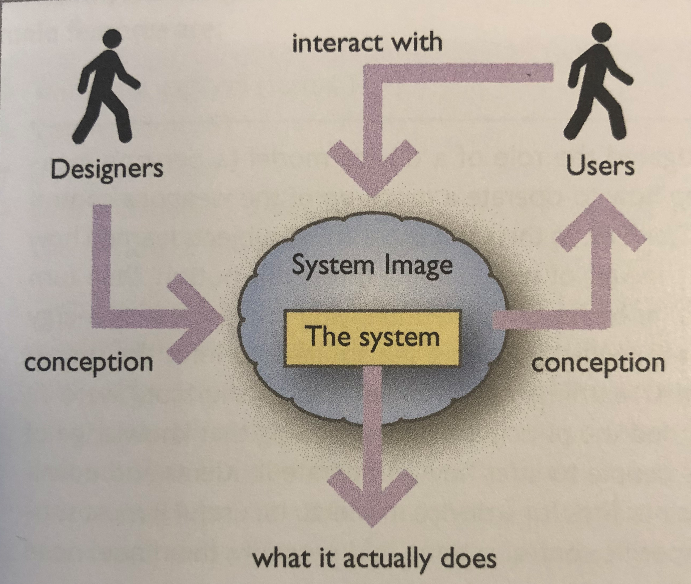
\includegraphics[width=0.4\textwidth]{billeder/SystemImage-Benyon.png}
	\caption{\textit{The System Image from \citep[p.~31]{Benyon}}}
	\label{fig:PACT-SystemImage}
\end{figure}
\todo[inline]{Anna: Scan billedet ind i stedet}

The PACT theory presentation and analysis will be written congruently throughout this section.
First the specific theory will be presented followed by the analysis.

\subsection{People}\label{sec:PACT-people}
People differ from each other in many ways.
This element in the PACT analysis is a way to ponder upon these differences as well as a way to categorize the different users of a system.
Three differences usually discussed in this part of the analysis are; \textit{physical, psychological}, and \textit{social}.
In this chapter we will discuss physical and social differences.

Physical differences covers the relevant ways people differ in physical characteristics.
This could be, differences in perception from the five senses; sight, hearing, touch, smell and taste as well, along with age, height or weight.
An example of a physical difference could be color blindness, which affects about $8\%$ of men and $0.5\%$ of women in the world \cite{ColourBlind}.

Social differences is about how people use a system for different reasons and therefore can have various goals.
Additionally, there is also a big difference in people's expertise levels which affects how an interface might be designed.
This is an important consideration since designing a system for a homogeneous group of people is  different from designing one for a heterogeneous group.

In the case described in this report, see \cref{sec:CaseDescription}, there are four main groups of people that need to be considered.
These are the quality manager, secretaries, department heads, and everyday workers.
This is a heterogeneous group with IT experience ranging from possibly none to what is required at everyday office work.
Should a worker have no IT experience it seems reasonable to assume that this worker may be cautoius of it and the design needs to take this into account.
The group also has different levels of domain expertise ranging from novice to expert which needs to be considered.
The quality manager is a domain expert and therefore has different needs of the system than the everyday worker with no expertise.
Furthermore, issues such as colorblindness, other handicaps, as well as bad memory needs to be considered when designing the system and interface.

\subsection{Activities}\label{sec:PACT-actvities}
\todo[inline]{Andreas: Omformuler ``when considering'' PS: bearing in mind}
Each actor in the system has a different use of it
% Ved ikke om det er mening at den ovenståede sætning skal stå der?

It is important to figure out what activities the system need to support.
First and foremost, the analysis of the activities should focus on the overall \textit{purpose} of the activity.
However each one of the groups described in \cref{sec:PACT-people} has a different goal in using the system.
The quality and department managers need to manage, update and access the handbook, whereas the workers only need to access and read certain documents.
This will be further elaborated in \cref{sec:Actors}.
The different kinds of purposes an activity can have is explored below.

\todo[inline]{Anna: Tilføj department manager, og hvorfor write eksisterer. Men først når der er flyttet rundt i ting}

\textit{Temporal aspects} covers different features in the system as well as a consideration of how the users' interactions with the system are done during a day.
Starting with the considerations of user interactions, one need to consider among other:

\begin{itemize}
	\item How often is the interactive system used?
	\item Is the interactions with the system done continuously or interrupted?
\end{itemize}

For the temporal aspects in a given system the developers need to consider things such as; time pressures, peaks and, and the response time of a given activity.

\textit{Cooperation} is simply the consideration of whether or not the activity is done in cooperation with others, alone, or a mix hereof, as well as how and when a possible cooperation is needed.
This is an important consideration since a system which is done in cooperation with others needs to have an awareness of all the users, be able to coordinate it between them and maybe have a communication system implemented as well.
On the other hand if the activities are done completely alone these features are not necessary.

\textit{Complexity} describes the question of how well-defined the activity is.
Is it a well-defined task which can be done in a simple step-by-step design, or is it a vague task, which would require the users browse around?

\textit{Safety Critical} has two sides to it.
First is whether or not the activity in itself is ``safety-critical'' where mistakes could be reason for injury or serious accidents.
Second is the consideration of ``what will happen when mistakes and errors are made?'' which is important for any developer to reflect upon and then design for these circumstances.

\textit{The nature of the content} is a more technical reflection of which data requirements are needed for the activity as well as what media it requires.

% Kunne det være en ide at lave en subsubsection ved navnet "Activities of OBHandbook" eller noget da activities del er ret laaaang
In the case of this project in terms of temporal aspects during the activities users may experience interruptions and the system should therefore be simple to use and easy to get back to.
Being easy to use is a feature most relevant for the everyday workers, as they only occasionally need to read documents and therefore are less in contact with the system.
This makes it necessary to make the system as easily accessible for them as possible.
The activities would most often be done during business hours, from 8-16 on weekdays, though may be accessed outside of this time frame as well.
\todo[inline]{Rasmus: Skriv om notifikiationer}
% Taniya: kunne måske være en ide at kort nævne administrator at selvom de bliver forstyrret med notifikationer fra systemet så skal admin hurtigt kunne vende tilbage til arbejdsopgaven admin var i gang med.
%Men stadig nemt kunne se/huske/ finde tilbage til de notifikationer, så de hellere ikke bliver glemt.

The cooperation aspect is mostly relevant for the administrator and writer roles as they are maintaining the handbook documents.
Here it is necessary to not only write new versions of a document but also make sure that the newest versions are approved.
Though writing the documents in itself does not require collaboration.
However, after a document has been written, it needs to be approved by other users.
This is one of the most important collaboration aspects in the system.
As for the worker's activities, there is no cooperation involved as all the workers need to read the newest, relevant documents individually.

Regarding complexity in this project, the activities are quite well-defined overall.
For the administrative personnel it is well-defined that whenever a new document has been written, it needs to be approved and then added to the handbook.
Here the oldest, and now outdated, document is being archived and stored.
The department manager needs to make sure that the affected everyday workers read and understand the new documents.

In relation to safety critical, there are no physical safety issues to consider in relation to the system, though there are serious consequences to consider if the handbook documents do not live up to regulations.
It is required that there are updated handbook documents and that the archived versions of these documents are stored somewhere.
If this is not upheld then the firm could suffer loss of certification, see \cref{sec:standards}, which would result in great loss of revenue.

In terms of the nature of the content, the system should be able to handle Microsoft documents such as Word and Excel as these are the filetypes used to write the documents.
As Ipsen has mentioned, it is also acceptable that the system accepts PDF files instead, as long as she is able to write the document with her preferred text editing software.
Furthermore the system should support large quantities of these files as the archived versions of the documents are usually stored indefinitely.

\subsection{Contexts}
Activities always occur in a context which will be explored in this section.
Context can be thought of, as something that surrounds activities as well as a feature which binds them together into a whole.
Usually when considering this point in PACT the three points: \textit{Physical environment, Social context}, and \textit{Organizational context} are at the main focus.
The analysis will not touch upon the social context as this is not considered relevant for the system development.
This is because the system is developed for a business and work context and does not consider the social interactions of the users for maintaining the handbook documents.

The physical environment might cover everything from weather to geographical placement of where the activity is done.
It is an analysis of the surrounding environment which may have effect on how users perform activities.

There are two main physical contexts to consider.
For the quality manager and the secretaries an office context is most likely as they handle administrative work.
For the everyday workers the context could differ dramatically as their functions may differ from each other.
The main focus here is that the handbook documents should be easily accessible, no matter in which context the workers are located.
Previous to this development project, the most common way that the handbooks were used by employees were in a paper format, which allowed the use of the documents in circumstances not conductive to electronic equipment.
It is expected that this practice will continue after the project.

As for the organizational context there are different factors to consider.
These are Ipsen who acts as a third party quality manager for a firm in relation to maintaining the handbook.
Then there is the in-house secretary who Ipsen works the closest with.
There's the CEO who from time to time reads, writes, and approves the handbook documents.
Lastly there are the everyday workers within the firm whose work and daily tasks vary depending on their positions.

It is because of the structure of the organization that there needs to exist different access rights in the system which are administrator, writer, and reader.
The administrator role is mainly for the quality manager who is the main person to manage the handbook documents.
There are actors within the firm, the CEO for example, who occasionally needs to write/update documents in the handbook and need writer access rights.
All of the workers need to read and understand the specific documents in the handbook that relates to their work.
These workers need reader rights to access the documents.

\subsection{Technologies}
\todo[inline]{Henrik: Find nogle nye øjne, og Giv så technologies et kærligt hånd}
Technologies is the reflection on the medium which interactive system designers work with.
It covers looking into elements such as what medias and technologies are needed to best get input and present the output, and review the communication between the needed devices.
Furthermore, it also examines the content, which concerns the data in the system and its form.
Good content is defined as accurate, up to date, relevant and well presented.

Since the activities are most often done in an office environment, on a standard PC, the input medias are keyboard and mouse.
In addition output is presented through a monitor, or for the workers on the factory floor through a printed version of the handbook, or parts of it.
The contents on the monitor are presented through a Graphical User Interface (GUI).
Furthermore, the communication user-to-user is usually done through telephone, while it between devices is done over a network, such as the internet.
Lastly, the communication from the system to a user is done through notifications.


\section{Usage}\label{sec:Usage}
\todo[inline]{Andreas: Vejleders tidligere kommentar omkring Usage afsnit skal rettes til}

In this section the usage of the system will be analyzed.
Who uses and how they use the system will be explored systematically through analyzing who the actors are, and the use cases of the system.
The actors consists of the different user groups who will be utilizing the system and the use cases will describe the different uses the system will potentially have.

The actors that have been identified within the case are \textit{administrator, writer}, and \textit{reader}.
%It should be noted here that the software in this context refers to the software that is under development throughout this project.
%This will outline what responsibilities that the system will eventually have when it is deployed.
The use cases of the system have been identified to be \textit{manage documents, manage users, manage departments, approve new documents, read status}, and \textit{track differences between document versions}.

An overview of the relationships between the actors and the use cases are shown through the table below, \cref{tab:UseCases}.
Here it is outline which actors have which responsibilities in relation to the system.

\begin{table}[H]
	\begin{center}
	\begin{tabular}{| m{10em} | c | c | c | c | c |}
		\hline
		& \multicolumn{3}{c|}{\textbf{Actors}} \\
		\hline
		\textbf{Use cases} & Administrator  & Writer & Reader \\
		\hline
		Manage documents & x & & \\
		\hline
		Manage users & & x & \\
		\hline
		Manage departments & & x & \\
		\hline
		Approve new docs & & x & x \\
		\hline
		Read documents & & & \\
		\hline
		Track differences\newline between document\newline versions & x & x &\\
		\hline
	\end{tabular}
	\end{center}
	\caption{ {\color{red}husk at sætte caption og label så den kan referes til} }\label{tab:UseCases}
\end{table}
\todo[inline]{Anja og Astrid: Efter actors og use cases er paa plads, saa skal vi lige kigge paa tabellen igen.}
\todo[inline]{Astrid: Tænker at vi er nødt til at tilføje en use case omkring at læse dokumenter eller noget fordi det ikke rigtigt giver mening at have en aktør der intet kan.}

In the rest of this section both the actors and use cases will be elaborated, starting with the actors.

\subsection{Actors}\label{sec:Actors}
\textbf{Administrator}
\textit{Goal}: Manages document versions, users, and user departments.
\\
\textit{Characteristic}: There is at least 1 administrator per handbook who administrates the documents and the users who has access to the handbook.
\\
\textit{Examples}: The administrator has access to all parts of the system which includes the archive, users, editing users, updating the documents and so on.

\textbf{Writer}
\\
\textit{Goal}: Update specific documents in the handbook.
\\
\textit{Characteristic}: One or more employees who need to update one or more documents in the handbook.
\\
\textit{Examples}: When someone, who is not the administrator, needs to update one or more documents they get temporary writer access rights.

\textbf{Reader}
\\
\textit{Goal}: To read and understand documents in the handbook
\\
\textit{Characteristic}: There are many readers who have various positions in the firm. Their shared characteristic is that they all need to read parts of the handbook.
\\
\textit{Examples}: When a document has been updated all affected readers must read the newest version and understand the difference between the previous and current one.

\subsection{Use cases} \label{sec:usecases}
\todo[inline]{Taniya: Tegn nogle statecharts, og få Anna til at tikze dem}
\todo[inline]{Astrid: Konkretiser use cases}
\todo[inline]{Andreas: Sikr tiden real quick}
\todo[inline]{Rasmus: Lav nogle ordentlige aktører. Reader, writer, administrator}
\textbf{Manage documents}
\\
It is desired that a handbook containing several documents and their versions is managed by a software.
This includes a TOC from which users are able to have an overview of the documents.
There are active and inactive documents, where the active documents consists of the newest versions of the documents, and inactive ones are archived.
The system also provides the person adding new versions with the option to write a changelog, where the user can write why there are changes to the document.

\textbf{Manage users}
\\
It is the administrator and software's responsibility to manage users and their administrative rights.
The administrator updates the system by adding, editing or removing users, while the software stores the users and their data in a database.
There are three types of users with varying degrees of administrative rights.
The administrator is able to create, edit, and delete users.

\textbf{Manage departments}
\\
The administrator manages departments within the system.
The administrator is able to create, edit, and delete departments by adding or removing users from them.
A department is subscribed to one or more documents which are relevant to the users within the department.
A user can be within one or more departments at once.
The software is responsible for notifying the departments whenever a document has been updated.

\textbf{Approve new documents}
\\
Whenever a new version of a document is available, it needs to be approved by one or more persons.
The user(s) who is responsible for approving the document(s) could either be the manager, or blue-collar worker.
When a document has been approved it is updated within the system, the older document is archived and the TOC is updated.

\textbf{Read status}
\\
Whenever an updated document is available, the subscribed departments are alerted.
All users within the subscribed department must read and understand the new document version.
When this is done, they check off box which indicates to the system and secretary that the new document has been read.
\todo[inline]{Henrik: Henrik: Der skal generelt henvises til tidligere tekst + er lidt forvirret mht consultant}

\subsection{Actors}\label{sec:Actors}
The actors exist in the application domain and as such are not within the system but interact with it. They are defined as

\begin{defn}
An abstraction of users or other systems that interact with the target system. \citep[p.~121]{Rod-Aalborg}
\end{defn}

The roles in the system were described and explained in \cref{sec:user} and it was visualized with \cref{fig:RoleIllustration} how the roles encapsulate each other.
However based on \cref{tab:ActorTable} it is clear that this is mostly but not entirely true, as the administrator cannot mark a document as read but reader and writer both can.

This is because the administrators have no need for this functionality as none of them work in the production, which can be seen in the examples in \cref{tab:Actor-admin}.
The quality manager has written or approved the documents and therefore obviously knows what they contain.
The secretary does not need the actual documents only the administrative access to the system and possibility to help other users.
The CEO needs to be in the system to approve documents but has no other use of it.

\begin{table}[H]
	\begin{tabular}{l m{11.3cm}}
		\hline
		\multicolumn{2}{c}{\textbf{\textit{Administrator}}}\\
		\hline
		
		\textbf{Goal} &  Manages document versions, users, and departments. There is at least 1 administrator per handbook\\
		 &  \\
		 
		\textbf{Characteristic} & Someone in the company in an administrative or leader position.\\
		&  \\
		
		\textbf{Example 1}
		& The quality manager is comfortable using the system. 
		They are responsible for maintaining and updating the handbook.
		They write the majority of the documents, approves the rest and has a complete overview of the entire system at all times. \\
		&  \\
		
		\textbf{Example 2}
		& The secretary rarely uses the system.
		They have an administrative role in the company and therefore needs complete access to all of the company's systems.
		They mainly create new users and every now and then search for a specific piece of information.\\
		&  \\
		
		\textbf{Example 3}
		& The CEO of the company has this role only out of formalities and usually acts like a reader\\
		
		\hline
	\end{tabular}
\caption{Actor specifiactions for \textit{Administrator}}\label{tab:Actor-admin}
\end{table}

The department head knows more about their own department than anybody else, and are both among the first ones to know when an update is needed as well as one of the people best equipped to write said update.
Furthermore, the quality manager cannot write the entire handbook due to its size and needs a writer to do some of the heavy lifting.
However, they also do not wish to grant the level of access to the system that an administrator role gives everytime someone needs a little more functionality than the very limited one the reader role offers.
This introduces the need for the \textit{writer} actor, as seen in \cref{tab:Actor-write}.

\begin{table}[H]
	\begin{tabular}{l m{11.3cm}}
		\hline
		\multicolumn{2}{c}{\textbf{\textit{Writer}}}\\
		\hline
		
		\textbf{Goal} & Update specific documents in the handbook. \\
	 	 &  \\
	 	 
		\textbf{Characteristic} &  One or more employees who need to update one or more documents in the handbook, but is not allowed all-access to the system. \\
		 &  \\
		 
		\textbf{Example 1} 
		& A department head updates the documents connected to their own department and sees that everyone in their department has read those documents.\\
		
		\hline
	\end{tabular}
	\caption{Actor specifiactions for \textit{Writer}}\label{tab:Actor-write}
\end{table}

The everyday worker only needs to read and mark documents as read and therefore that is the only functionality they have.
They are a very broad group both in terms of willingness to use the system and ability to use the system to its full capacity.

They may be an experienced IT user excited to try out a new system.
They may also be someone who does not use IT very much in their daily life and as a result is vary of technology in general.
Or an old worker who has done this job for 30 years and sees no reason to change their workflow.
They can come from anywhere in the firm and may be one of the higher-ups or someone who is used to office work.
However they may also be a production worker and not even have a work related e-mail or phone number.

\begin{table}[H]
	\begin{tabular}{l m{11.3cm}}
		\hline
		\multicolumn{2}{c}{\textbf{\textit{Reader}}}\\
		\hline
		
		\textbf{Goal} & To read and understand documents in the handbook. \\
		&  \\
		
		\textbf{Characteristic} & Can come from all levels and areas in the company.
		Their only shared characteristic is that they all need to read and confirm that they have read certain parts of the handbook.
		They may not have a work related e-mail or phone number.\\
		&  \\
		
		\textbf{Example 1}
		& The worker who is an experienced IT user and has both e-mail and phone number connected to the system.
		They check for notifications regularly.\\
		&  \\
		\textbf{Example 2}
		& The worker who is not an experienced IT user and as a result is vary of it. 
		They only use the system when absolutely necessary and may not see a notification when it comes.
		They may be vary of the system due to their inexperience with technology.
		They do not have e-mail nor phone number connected to the system and would likely not see a notification in due time even if they had.\\
		&  \\
		
		\textbf{Example 3}
		& The production worker who does not have a work related e-mail or phone number. They do not get notifications at all, and rely on the department head to know when an update is out rather than notifications.\\
		&  \\
		
		\textbf{Example 4}
		& The CEO when they are not an administrator out of formalities only needs the level of access that a regular \textit{reader} has.\\		
		
		\hline
	\end{tabular}
	\caption{Actor specifiactions for \textit{Reader}}\label{tab:Actor-read}
\end{table}

One of the reasons why every role has the right to approve an addition or update to the handbook is that the CEO's main job within the handbook is to do exactly that.
However they do not need to do anything else in the handbook and therefore needs only the minimum level of access.
That and there is no need to restrict the functionality to a specific role as the users need to be specifically assigned to approve anything anyway.
\subsection{Use cases} \label{sec:usecases}
\todo[inline]{Anna: Tikz taniyas seje statecharts}

\textbf{Access current handbook}
\\
\textit{Any actor} can access the handbook by going to the website where it is located where they need to log in with username and password.

If it is the first time they log in they are automatically led to the settings page.
Here they need to change their standard password and have the option to update their e-mail address and phone number.
They are redirected to the front page, when they click confirm.
If it is not the first time, they are led directly to the front page.

Documents relevant to this specific user are shown first.
Below all the chapters are visible.
A user can view the documents in a chapter by clicking unfold on that specific chapter.
Alternatively they can unfold all chapters by clicking unfold all.
When they click on a document a preview is shown if the file is a pdf.
Otherwise they have the option to download the file.
The changelog from last version to current version is shown above the preview.
Depending on the user's role further actions are available in this view (elaborated in other use cases).
To exit the view the user clicks outside the box or the x in the corner.

\input{Chapters/ApplicationDomain/Access-Fig}

\textbf{Add new file to the system}
\\
An \textit{administrator} or \textit{writer} can add a new a document by clicking an upload button on the front page.
They are then taken to a seperate menu, where they specify the file which they wish to upload.
They can select an existing chapter from a drop-down menu or create a new one. 
They can then either choose an existing ID and title or create a new one.
If they create a new one the uploaded file becomes the first version of this document.
If they choose an existing one the uploaded file is added to the document as the newest version.
Depending on the system settings they may also be prompted to write a changelog for the new version.
In both cases they will be prompted to choose the people who should approve this addition to the handbook.

After clicking 'Send for Approval' the view returns to the front page and they now have the document in their relevant documents.
They have the option to delete it until it has been approved.
After it can only be archived by adding a new version.

Another way to add a new version to the document is from the preview of a specific document.
In this case they are not prompted for chapter, existing ID or title as those are already defined.
The rest of the flow is the same.

\input{Chapters/ApplicationDomain/Add-Doc-Fig}


\textbf{Approve new version or document}
\\
\textit{Any user} can be set as an approver to a document.
When a user has been set as an approver they get an email notification about this.
Once they log in the document is shown in their relevant documents section.
They can then click on it to view and approve.
They can also click approve straight from the front page.
Once they have approved the document it is updated with a new version.
The former version is labeled as inactive and can be accessed through the archive.

\textbf{Access archive}
\\
The \textit{administrator} can access the archive by clicking on the archive in the sidebar menu.
The archive looks like the front page:
All of the chapters and their titles are visible and each has a drop-down menu containing all of the documents.
When a document is clicked a list of versions all versions of this document shows along with all the changelogs.
The administrator accesses a specific version by clicking it.
If the version is a pdf a preview is shown.
If not a download option is also available.

\textbf{Add user}
\\
An \textit{administrator} can add a new user to the system.
This is done by clicking 'User administration' in the sidebar and choosing the 'Add user' button.
A user needs needs a user name and a name.
A name can either be an actual name or an identification number.
It is possible to provide contact information in the form of e-mail and/or phone number.
A standard password is automatically set.
Once the administrator has clicked 'Add user' the new user is in the system and the administrator is returned to the User administration view.

\textbf{Edit user information}
\textit{Any actor} can edit their own information by clicking the cogwheel in the right corner.
They have the option to add, remove or change their e-mail address and phone number.
They can also change their username and password.
The changes are applied when they click confirm.

\input{Chapters/ApplicationDomain/Profile-Fig}

\textbf{User management}
\\
The \textit{administrator} can change information about all users in the system.
They access all the information by clicking 'User management' in the sidebar.
By clicking a user they access a menu where they can change a user's name, e-mail address and phone number.
An administrator can also reset a user's password.
The changes take affect once they click confirm.
They can delete users both from that menu and the overview.
When a user is deleted only the name remains in the database.
When they delete a user they get a popup asking whether they are sure.
The user is deleted once they click confirm and the popup disappears.

\input{Chapters/ApplicationDomain/User-Man-Fig}

\textbf{Mark document as read}
\\
A \textit{reader} is alerted to a new document they need to read through an email or sms notification.
They access the document by logging into the system and finding the document in their relevant documents.
Once they have the document open in preview they can mark the document as read by clicking the 'Read' button.
The reader can also elect to download the document to read it rather than read it in preview.
Should they do so the 'Read' button is also accesible from the front page.
A popup menu stating that they have read and understood the content of the version will pop up.
The reader then clicks 'Agree', the popup disappears and the read status has been saved.

\textbf{View who has read a document}
\\
The \textit{administrator} can view a specific document in preview.
Here a button called 'Read Status' is available and by clicking it a pop-up appears.
In the popup everyone connected to the document who has read it and who should have read it is listed by name.
They exit the popup by clicking outside it or on the x.

\input{Chapters/ApplicationDomain/ReadStatus-Fig}

\textbf{Manage departments}
\\
An administrator can access 'Manage departments' through the sidebar.
When they add a new department they need to provide a name and are then returned to the 'Manage department' view.
They can then click a department to view a list of all connected users sorted by name and a list of all connected documents sorted by number.
They can click edit user and are redirected to a menu where all the users in the system are listed.
They can then tick them on and off to select which users are connected to the department.
Similarly an 'Edit departments' button exists where they are then redirected to a list of all active documents in the handbook.

Worth noting. The administrator can change a user's name while the user themself can change their user name.

\input{Chapters/ApplicationDomain/Dep-Man-Fig}

\section{Functions}
When creating a system it is vital to get an overview of the functions and to determine the complexity of these functions. This is done by analysis of functions, in which the first step is to identify all functions. The result is a list of functions with a related complexity and type.

To begin the analysis a look at the system definition and use cases is necessary as it creates a template of functions that are ready to be analysed. The next step is then to determine what type each function belong to, this means determining if it is an \textit{update, signal, read or compute function}.

The most present type of function present are of the update type. These are described in the OOA\&D as "Update functions are activated by a problem-domain event and result in a change in the model's state."\citep[p.~140]{Rod-Aalborg}

The reason in this is in the nature of the system, as it primarily lies in management of users and documents. This also means that the complexity is mostly simple as the margin for error is rather small in these cases. 

Only exceptions are "Manage documents", where the complexity is in the validation where overlapping of information is not allowed. Furthermore "Track differences between document versions" can be difficult as different file types can be used by the users.

The "Notify user" is of the type signal, a function type that responds to changes inside the system.

"Track differences between document versions" is of the type read as it retrieves information from each document and presents the differences to the user.

This is the resulting table of functions:

\begin{table}[H]
\centering
\begin{tabular}{lll}
Function                                    & Complexity & Type    \\
Manage documents                            & Medium     & Update  \\
Manage users                                & Simple     & Update  \\
Manage departments                          & Simple     & Update  \\
Manage suppliers                            & Simple     & Update  \\
Approve new suppliers                       & Simple     & Update  \\
Approve new documents                       & Simple     & Update  \\
Update TOC                                  & Simple     & Update  \\
Track differences between~document versions & Medium     & Read    \\
Notify user                                 & Simple     & Signal  \\
Read status                                 & Simple     & Update 
\end{tabular}
\caption{Function list}
\end{table}


%Usage
%Functions
%Interfaces????

\chapter{Design}\label{design}
\todo[inline]{Anna: skitser, navigation structure tree}
The aim of this chapter is to design the architecture components which will eventually guide the implementation of the system.

This chapter is divided into the following parts: Architecture Design, Application Method, and Component Design.
The Architecture Design in \cref{sec:architecturedesign} will introduce and discuss the criteria and the requirement priorities.
In the Application Method section, the main framework that the system will be implemented within is introduced and discussed.
This will be followed by the framework that has been chosen for the implementation of the system.
In Component Design in \cref{sec:componentdesign} will introduce the theory for component design followed by the project's architecture component design.

\section{Architecture Design} \label{sec:architecturedesign}
In this section all of the pieces needed to be able to make the final component design are presented.
It starts with the system's criteria in \cref{sec:architecturecriteria}, followed by a prioritization of the system's requirements with the help of the MoSCoW rules in \cref{sec:requirements}.
After this, the system application framework is presented.

\input{Chapters/Design/architecturecriteria}
\input{Chapters/Design/requirements}

\section{Application Method}\label{sec:AppMethod}

\input{Chapters/Design/whyserver}
\input{Chapters/Design/aspnetcore}
\input{Chapters/Design/database}

\section{Component Design} \label{sec:componentdesign}

In this section the component design theory will be introduced and elaborated.
This theory will be utilized in the following section where the component design for the system will be presented.
%Anna: evt fjerne sætningen ovenfor da det virker til at være en gentagelse af den første

\input{Chapters/Design/architecturecomponents}

\subsection{System design} \label{sec:systemdesign}

In relation to the ASP.NET MVC pattern there are immediate similarities to the component design theory in \cref{archicomponents}.
There can among other be drawn parallels between the \textit{model} component and the \textit{model} classes in the MVC pattern.
The possible parallels are listed in the table below.

\begin{table}
	\centering
	\begin{tabular}{| c | c | }
	\hline
	\textbf{Components} & \textbf{MVC Pattern} \\
	\hline
	Model & Model \& EF Core \\
	\hline
	Functionality & Controller \\
	\hline
	Interface & View \\
	\hline
\end{tabular}
\caption{{\color{red}indsæt caption tekst}}\label{tab:PatternParallels}
\end{table}

As written in the component design theory in \cref{sec:archicomponents} the model components should seek to solve the problem of the problem domain.
%Anna: enten henvis til specifikke definition hvis sådan en eksisterer ellers henvis til afsnittet.
%Anna: Mener vi virkeligt "problem og the problem domain"
The model component in the MVC pattern is likewise going to contain the classes and objects that seeks to solve the problem domain through meeting the requirements written in {\color{red}section xx}.
The model component in the implementation is among other classes going to contain \textit{documents, users, departments, versions, approvals} and \textit{read statuses}.
The arguments for including these classes can be seen in \cref{sec:classdiagram}.
The database in form of EF Core is also included in the model component as this in part also seeks to solve the problem domain.
%Anna: Vi hrar endnu ikke introdyuceret denne forkortelse i brødteksten(EF core)

As written in the component design theory the responsibilty of the functionality is to provide the actor a means to access the model component.
%Anna: Henvis til afsnitet
%Anja: Der er blevet henvist i paragraffen ovenfor. Det begynder at blive overkill
The controller component in the MVC pattern does this by communicating between the model component and the view component.
The controllers retrieves data from the database and both methods and objects from the models.
Hereafter,it links these to the view.

The responsibility of the interface component is the handle the interaction between the users and the functionality.
This is done through the view model in the MVC pattern as the interface is handled in big part due to HTML, CSS and JavaScript.
These are what determines what the actors sees and what they can interact with.

\subsection{Component layers}
In relation to the theory written in \cref{archicomponents} the components can be designed in layers to describe their responsibilities and relation to each other.
The components in the MVC pattern with EF Core included can also be designed with the layered architecture in mind.
To give an overview and understanding of the architecture and design a simple component layer design can be seen in the figure below:
%Anna: synes den sidste sætning bliver en smule kringlet

\begin{figure}[H]
	\centering
	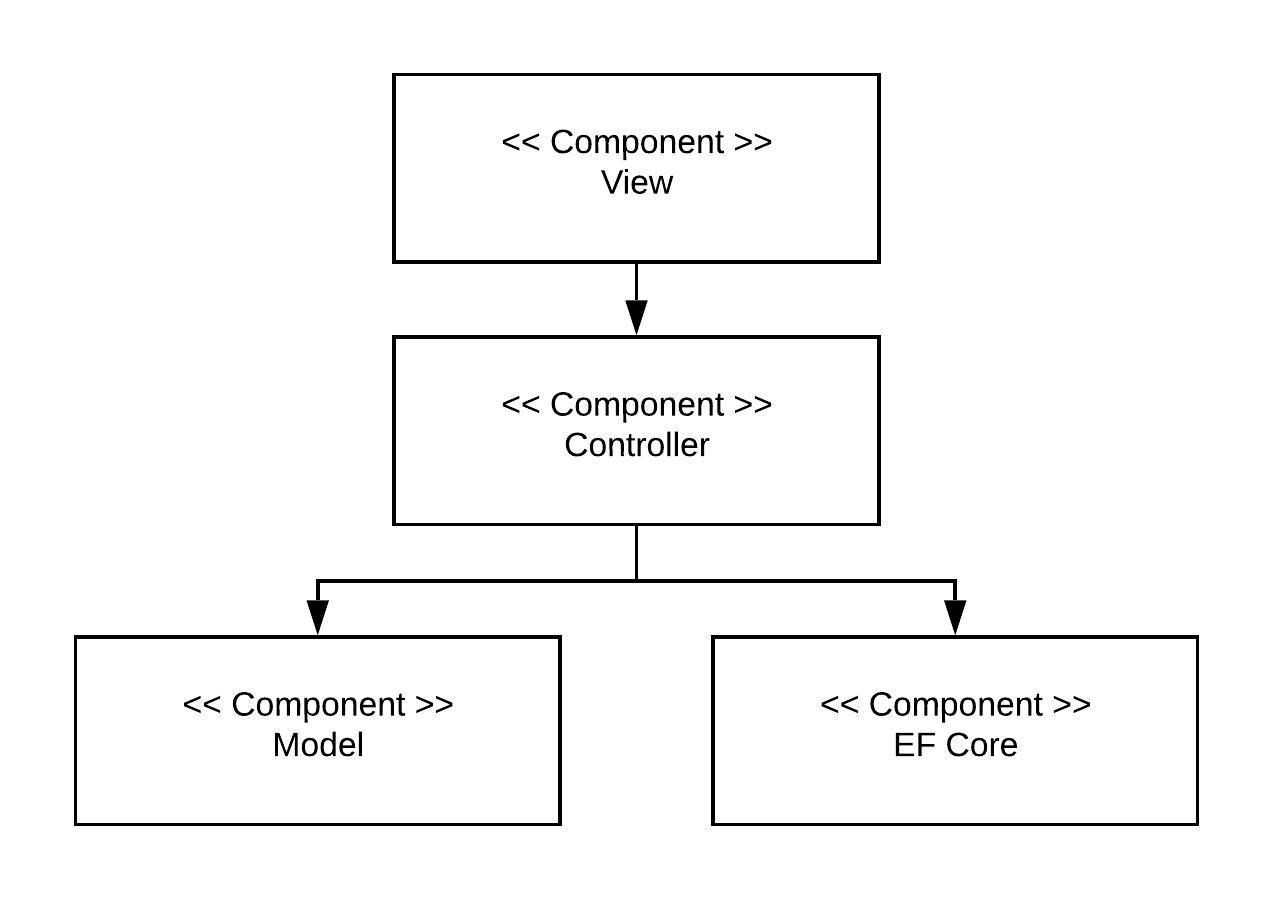
\includegraphics[width=0.7\textwidth]{billeder/simplecomponents.jpeg}
	\caption{Simple component layer design}\label{fig:SimpleComponent}
\end{figure}

View, controller, model, and EF Core are thus the main components layers that can be found in the design, each with a well-defined responsibility.
Ideally the architecture is designed so that the view and model components do not have to interact with each other.
% Kilde? Det virker lidt suspekt at views og models ikke skal kunne snakke med hinanden
% Anja: Virkelig? Tjah, saa tænker jeg slet sætningen ovenfor, da den er trukket ud af min røv
It is the intention that the controller is the link between these components, which is why it is placed in the middle of the layer components.
The main function of the controller is to link objects from the model component and data from the EF Core database and make these accessible for the view component.

%Anna: vil vove at påstå der ikke birde være et afsnit her
% Anja: Jeg vil paastaa det modsatte
This will not always be the case as the ASP.NET Core MVC model is designed so that a view has a corresponding controller.
For example the document view will have a corresponding document controller.
The document view will eventually have to borrow objects and data from other models in the system, which means that the view will at times have to bypass the controller component to communicate with the model component.

Subsystems can be explored from the main components, which e.g. are the interface system and its underlying technologies.
These are HTML, CSS, JavaScript and razor.
The model component has two main parts which are the model classes from the MVC pattern and the EF Core database system.
These two are defined as separate components which share similar responsibilities in the model component.
These components their relations with each other, and their underlying sub components can be seen in the complex version of the layer design below:

\begin{figure}[H]
	\centering
	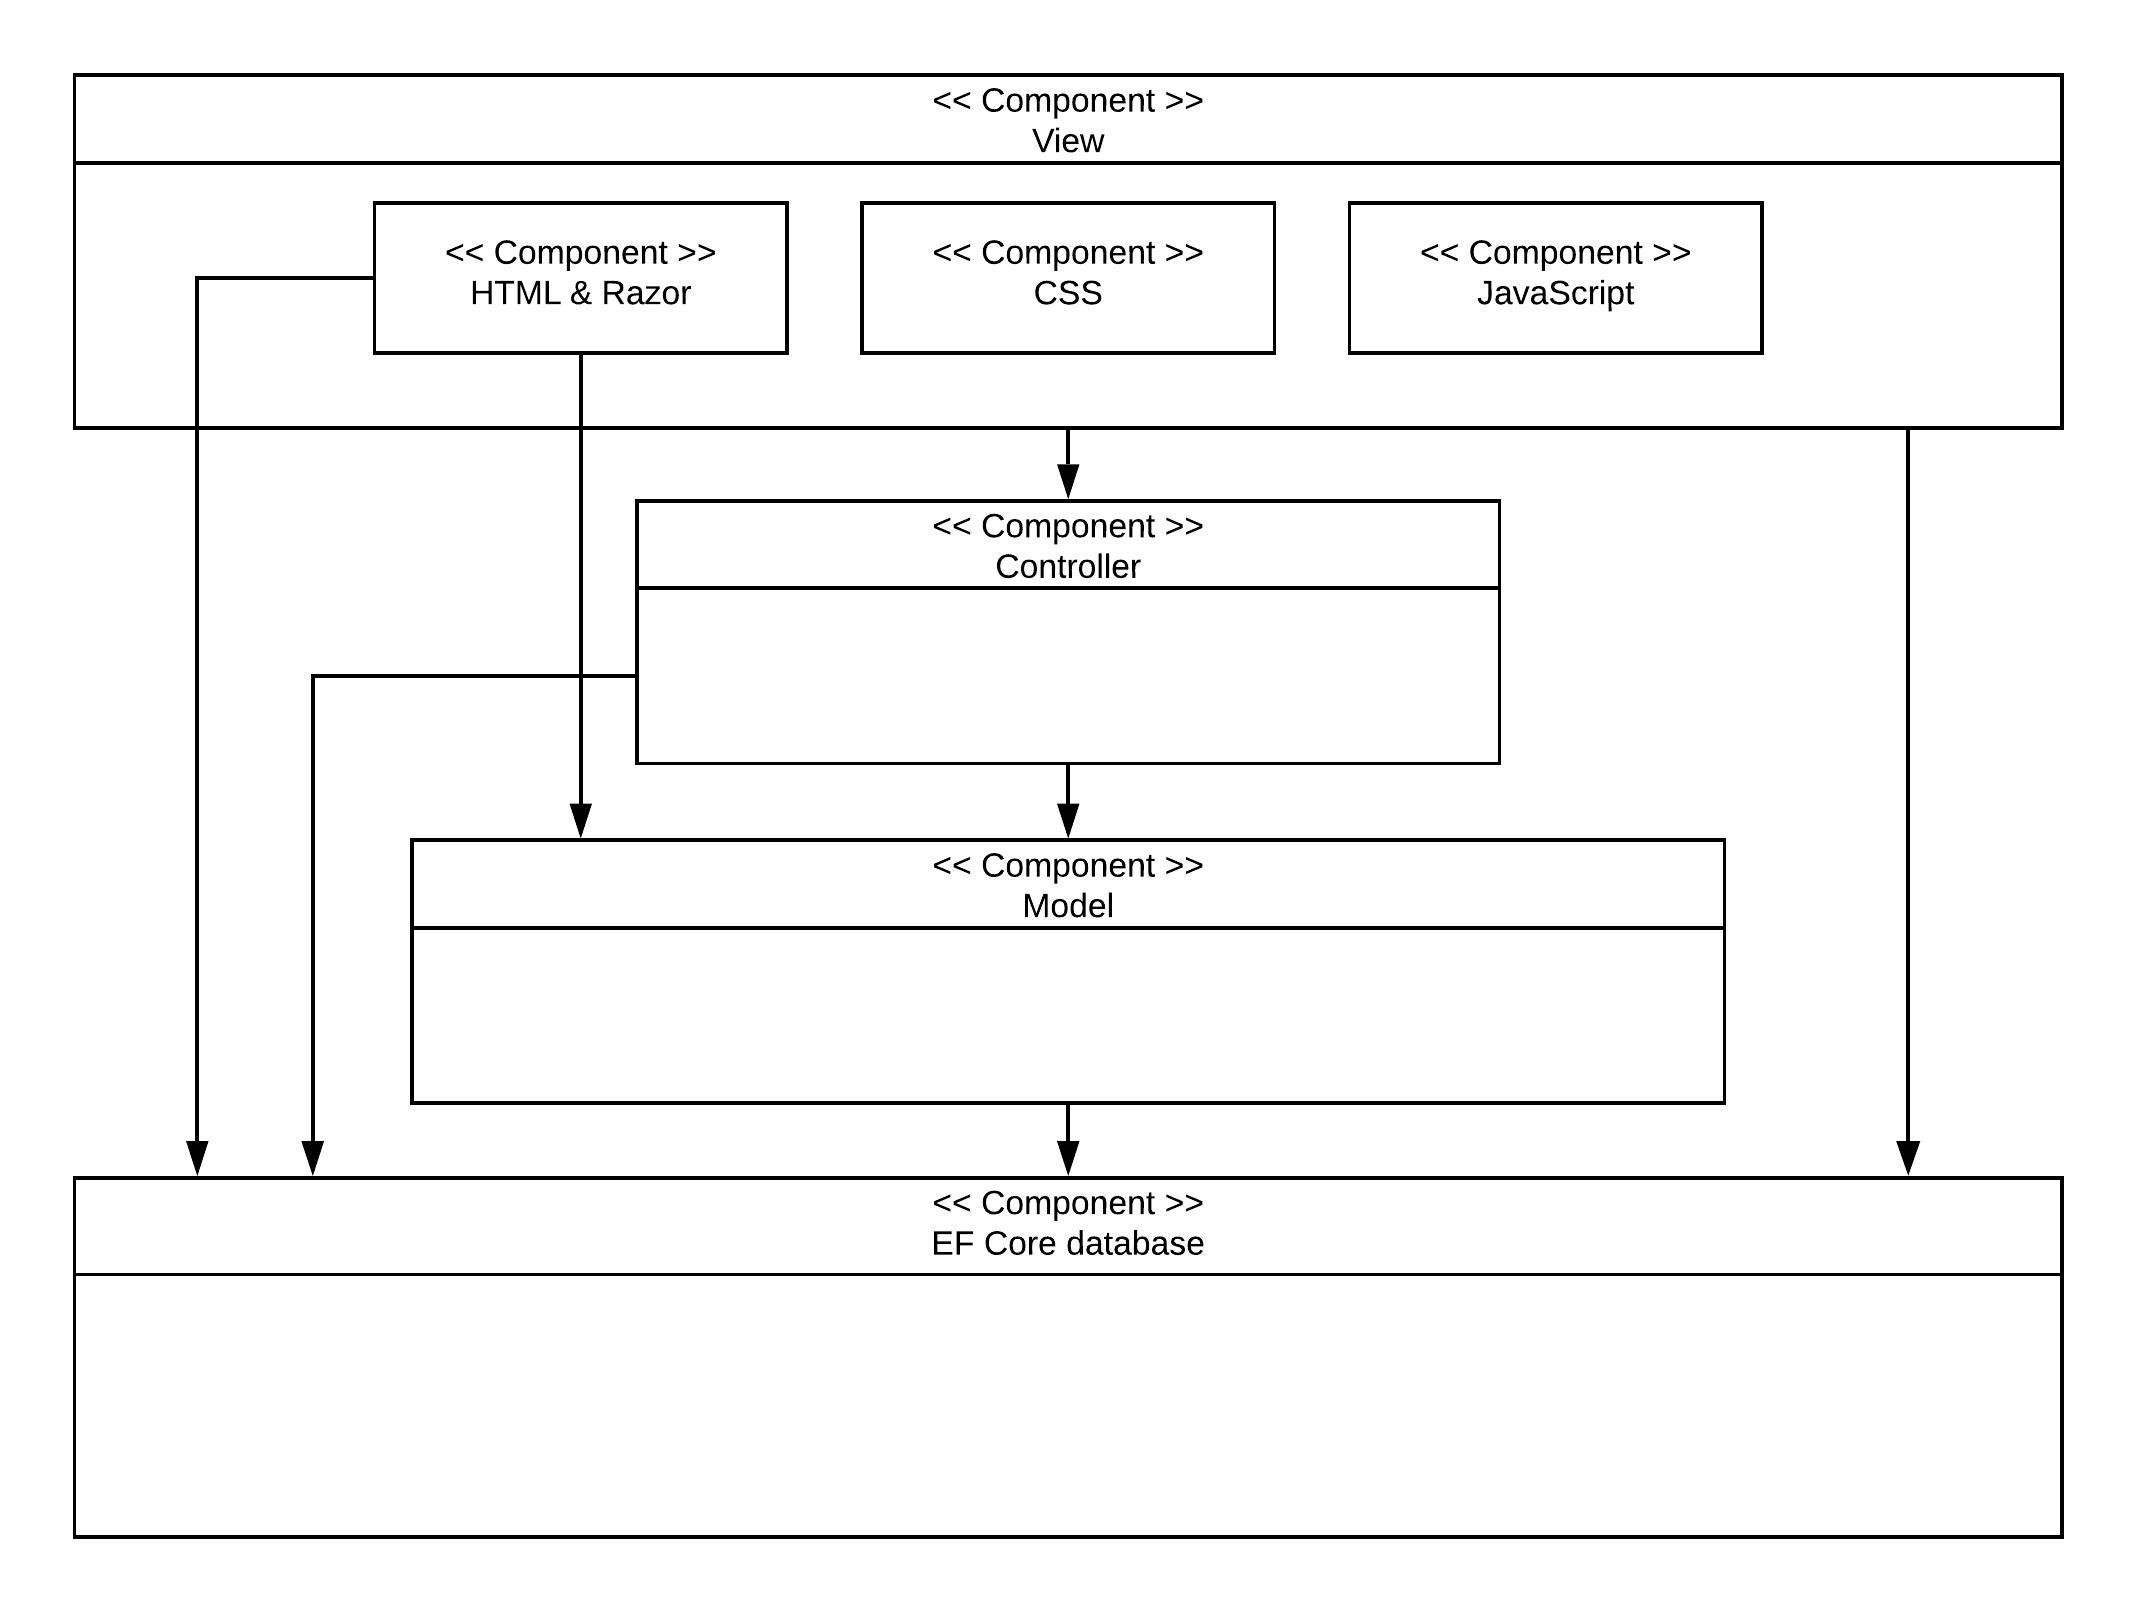
\includegraphics[width=1\textwidth]{billeder/complexcomponents.jpeg}
	\caption{Complex component layer design}
\end{figure}

Ideally the design would have \textit{closed-relaxed} architecture as the components would only be able to access layers adjacent to them.
In this design the design would be \textit{relaxed} as the controller would have access to both the view and the model components.
As it is though the design has an \textit{open-relaxed} architecture as the view component occasionally has access to the model component.
%Anna: Kan godt tænkes de to sidste sætninger trænger til en omskrivning
% Anja: Tjoh
% Henrik: Tænker at det er forkert med pil fra JavaScript til Model

In the final design there will be several classes included within each of the components.
Each of the main classes in the model component will have a corresponding controller and view in relation to it.
For example the document class in the model component will have a corresponding database in EF Core as well as a corresponding controller and view.
Here the documents object is within the model component and the documents data will be stored in the database.
A corresponding controller, which mainly handles the document class, ensures that the class and database are accessible for the actor.
The corresponding view ensures that the actor is able to see and interact with the document classes and database.

\section{Navigation Tree}
This section describes the navigation tree that visualizes how user move through the application, see \Cref{fig:Navigation}.
\input{Chapters/Design/navigation}

The user will first encounter the Login page.
For the first-timer user they have to enter the Activate account page and insert the given username received from administrator to register email address (optional) and create a password.
Once activate account process is finished user will be redirected to the handbook's Main page.
If the account is already activated user will be redirected to the Main page once logged in.

In the Main page administrator and writer will be able to access the ``Add new document'' page.
Writer will be able to access awaiting approvals under the relevant document section in the Main page.
Administrator will be able to enter the Approvals page through a sidebar which is only accessible for administrator.
The sidebar consists of:

\begin{itemize}
	\item Handbook (return to the Main page)
	\item Approvals
	\item Archive
	\item User administration
	\item Departments
	\item Settings
\end{itemize}

The Preview document page can be access in three ways depends on access rights, see \Cref{tab:docPreviewEntries} below.

\begin{table}[H]
	\begin{center}
	\begin{tabular}{| m{20em} | c | c | c | c | c |}
		\hline
		Document preview entry & Administrator & Writer & Reader \\
		\hline
		 Directly through document in the valid handbook & x  & x & x\\
		\hline
		 Through archive document  & x &  & \\
		\hline
		 Via awaiting approval document & x & x &  \\
		\hline
	\end{tabular}
	\end{center}
	\caption{Document preview entries}\label{tab:docPreviewEntries}
\end{table}

Through the User administration page which is accessible from the sidebar administrator will be able to access the Create user page or the User info page to enter the Edit page and update user information.

Under the Departments page entered through the sidebar.
Administrator will be able to click on existing department name to enter the Detail page of an overview of associate users and documents.
In the Detail page administrator would be able to enter the Edit users page or the Edit documents page.

The Settings page is accessible from the sidebar where administrator can change the company name and enable or disabled changelog functionality to the application.

In the Navigation tree in \Cref{fig:Navigation} the red box indicate that every role can enter the Edit profile page or Log out on the global, top-level navigation bar anywhere in the navigation flow within the red box.

%GUI

\chapter{Work flow}
%forskellige iterationer
Software Development Life Cycle (SDLC) is a way to systematically approach software development.
It provides a methodology to improve quality of the desired product and the general work progress. 
Depending on the customer or end users and how clear the project's requirements are different approaches are needed. 
Among the different SDLC methods are the most common ones the older traditional ''Waterfall model'' and the newer ''Iterative model''. \cite{SDLC-Toolsqa}


This chapter will first briefly present the ''waterfall model'' and the ''iterative model'', And during these the argument for choosing the ''iterative model''.
Hereafter, the chapter will contain a description of each iteration throughout the project.


\section{Waterfall model}
This section is based upon Sharma \cite{Waterfall-Toolsqa}, unless anything else is stated.
%smid bogens titel ind 
%Anna: Astrid det er ikke en bog men en hjemmeside

The principle of the waterfall model is that the software development process is divided into separate phases, which makes it a sequential design process.
Here the output, in form of documentation, of one phase serves as the input for the next one which means that no phase will start without the previous one being complete.
This is often illustrated as a downward going flow, see \cref{fig:Waterfall}, which is also the reason for its name.

\begin{figure}[H]
	\centering
	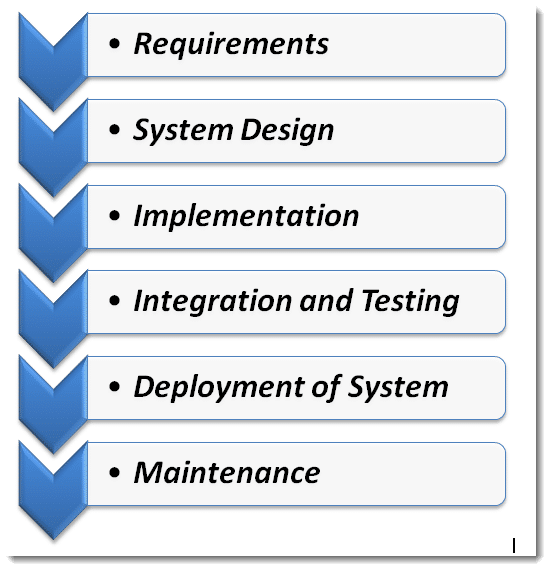
\includegraphics[width=0.4\textwidth]{billeder/WaterFall-Model.png}
	\caption{The Waterfall Model \cite{Waterfall-Toolsqa}.}\label{fig:Waterfall}
\end{figure}

\paragraph{The main benefits} of this model, is that it allows for departmentalization, which in theory makes it possible for separate teams to work at each phase without ever communicating with one another since only the documentation is necessary.
Another benefit of this system is how it is easy to manage since there are clear guidelines of what is needed before one phase is done and another can begin.

\paragraph{The main disadvantage} is on the other hand that because of this rigidity it becomes more difficult after every finished phase to go back and change things, when mistakes or misunderstandings of the concept has been made.
Therefore it is also not a beneficial model to use when there is a moderate to high risk that the requirements of the system changes.
%ville måske være bedre med en simpel textbf for at undgå ekstra mellemrum i pdfen
%Anna: Synes ikke selv det gør noget, kan god lide de to ting er skilt ad

Since the system developed in this project is done in cooperation with Ipsen, there is a moderate risk of the requirements changing.
This based on the risk of concept misunderstandings, since Ipsen is an expert in her field who has taken contact to software developers with no expertise in this field.
%ikke helt sikker på om jeg forstår this based delen af denne her sætning

\section{Iterative Model} \label{sec:iterativModel}
This section is based on sharma \cite{Iterative-Toolsqa} , and Sharp, Rogers and Preece \cite{InteractionDesign}, unless anything else is stated.
%vil igen argumentere for at der skal titel på
%Anna: det er ikke fordi det er normalt at gøre, normalt har man bare kilde referencen sat ind

The main principle of the iterative model is to divide the software development into a cycle of ''waterfalls'', it could also be seen as a form of ''multi-waterfalls'' model.
Instead of focusing on everything through every phase in the waterfall model, the development is done in pieces and at every iteration a little more is added to the product until it is finished.
The model usually has four basic activities, the formal names may change from the specific models but the idea is the same. 
Through each iteration the product and requirements are always being redetermined, redefined and further developed through the four main activities and in collaboration with the client or users, until the final solution is reached.
Different iteration models are simplified versions of reality and are not meant to be prescriptive, and depending on the project it is not always possible to go through all of the phases described in these models. 
Three explicit models will be presented in the \cref{sec:Iterative1,sec:Iterative3}.


\paragraph{The main benefits}
of working iteratively is the continuous talk with the client and users which yields the opportunity to determine and redetermine what their needs truly are rather than just what they believe them to be.
This ongoing communication also makes it easier for catching mistakes and faulty software since only a little part is added at each iteration.
It is easier as well to clarify misconceptions of the products requirements.
The repeated correspondence with the client and/or users is likewise the center of the user-centered approach, mentioned in \cref{sec:PACT}, which is of great importance when designing and developing an interactive system.
%måske få tydeligere frem at det er nemmere at opdage fejlene tidligere

\paragraph{The main disadvantage} of the iteration model is how adding functionality at every stage, may cause problems related to the system architecture since it had not been thought into the design to begin with.
This may in worst case scenario cause for the whole system to be redesigned at re-implemented.
Another disadvantage with this model is also one of it strong suits and allures, which is how it can become difficult to manage, and keep track of the development and when a iteration is done and a new one begin since it is ever changing.

\paragraph{Iterative model in design process:}
%Anna: Evt fjerne paragraph titlen ovenfor, er ikke sikker på om den i virkeligheden gør noget for det hele
As suggested in the disadvantages one of the allures of this iteration model is its ever changing quality and how it i more of a guideline which conforms to the different periods of the software development.
This suits the process of designing interaction system which is ''messy'' as the quote below from \citep[p.~156]{DesignerStance} illustrates.

''Remember, design is messy; designers try to understand the mess. They observe to how their products will be used; design is about users and use. They visualize, which is the act of deciding what it is.''

The Iteration proccess and the contentious communication with client and/or users is therefore a more natural way to develop human centered interaction systems.


\subsection{The process of designing interaction systems}\label{sec:Iterative1}
This section is further based upon Benyon \cite{Benyon}, unless anything else is stated.

As mentioned in \cref{sec:iterativModel} there are usually four basic activities, which may be called differently in the different models, even though the basic idea is commonly the same.
In life cycle model in \cref{fig:LifeCycleModel} these activities are called;
\textit{establishing requirements, designing alternatives, prototyping,} and \textit{evaluating}. 

\begin{figure}[H]
	\centering
	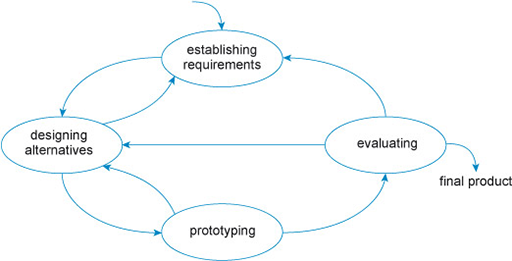
\includegraphics[width=0.75\textwidth]{billeder/lifecycle.png}
	\caption{Life cycle model \citep[p.~332]{InteractionDesign}}\label{fig:LifeCycleModel}
\end{figure}

To be able to design a system with the user’s needs and wants in mind it is imperative to know the target users and which activities the system needs to support. 
This is done through establishing requirements where information of the target users is gathered through data gathering and analysis. 
When the requirements are settled it is possible to design alternatives ideas that meet these suggested requirements. 
After the alternative design phase is completed a prototype can be developed. 
The purpose of the prototype is to evaluate with the users whether the criteria has been fulfilled and to present how the system could potentially turn out. 
Finally, when the prototype is complete it can be measured an evaluated. 
The evaluation phase determines whether or not the design is usable and/or acceptable and thereby if another design iteration is needed.

%Anna: tænker lidt vi enten bruger teksten ovenfor eller denne her nedenunder, synes det bliver meget dobbelt konfekt at bruge beggge.
According to Sharp, Rogers and Preece ''Most projects start with establishing requirements'' \citep[p.~333]{InteractionDesign}. It is from this first activity that it’s possible to go into the ‘designing alternatives’ activity from where a prototype in the ‘prototyping’ activity, can be developed which in turn can be evaluated by the users in the ‘evaluating’ activity. From this evaluation the designers can specify new or redefined requirements, or they can go directly to redesign or deem the project done. 

\subsubsection{Another take on the interaction design process}\label{sec:Iterative2}
In \cref{fig:DEBModel} another model is shown, where it becomes more apparent how it might be difficult to define when an iteration ends and a new one begin since it is possible to start and any point and to move back and forth between the activities seen fit.

\begin{figure}[H]
	\centering
	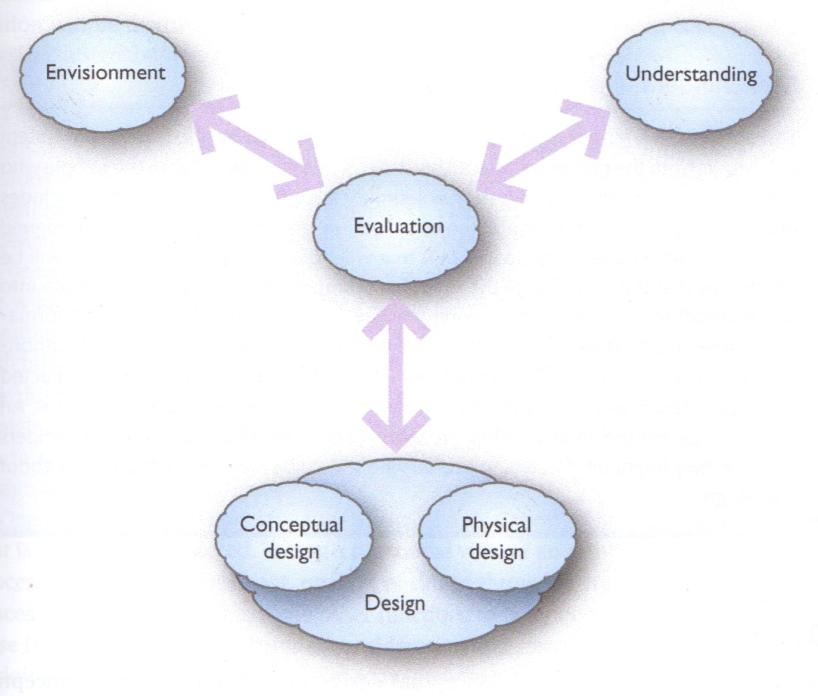
\includegraphics[width=0.5\textwidth]{billeder/DEBModel.jpg}
	\caption{Understanding, design, evaluation, envisionment \citep[p.~49]{Benyon}}\label{fig:DEBModel}
\end{figure}

The four basic activities of this model is instead of those shown above called; \textit{understanding, design, envisionment} and \textit{evaluation}.
though they correlate a lot with those before. 
'Understanding' is a broader term for 'establishing requirements' since it also covers topics such as understanding the context of the developed system and the technological landscape.
The 'envisionment' activity concerns itself with determining appropriate media in which to render design ideas.
While the 'design' activity is done through conceptual- and physical design as seen in \cref{fig:DEBModel}.
These two activities is together comparable to the 'designing alternatives' activity and 'prototyping' activity from \cref{fig:LifeCycleModel}.
'Evaluation' is the same in both models, it is the center of the process.

\subsection{OOA\&D iteration model}\label{sec:Iterative3}
This section is based on Mathiassen, Munk-Madsen, Nielsen and Stage \cite{Rod-Aalborg}, unless anything else is stated.

In the OOA\&D method the four basic activities are; \textit{Problem-domain analysis, Application-domain analysis, Architectural design} and \textit{Component design}.
In between these activities  also lies programming and quality assurance.
The importance of each activity is relative in each iteration and the sequence changes from each development project.
Further down in this section two different models based on the OOA\&D method is presented.

%Anna: er det nødvendigt at skrive et afsnit om sammenligning af de fire aktiviteter?, da det i princippet er modeller til to forskellige ting tænker jeg ikke det er nødvendigt explicit at skrive ind her

In \cref{fig:SUModels} two different models based on the OOA\&D method is shown.
The first model, \cref{fig:SUModel1} is a model closer to the traditional waterfall model though it is still an iterative process modeled.
The second model, \cref{fig:SUModel2} is on the other hand closer to the stereotype of a iterative model where each phase is done or at least considered in every iteration.

\begin{figure}[H]
	\centering
	\begin{subfigure}[b]{0.48\textwidth}
		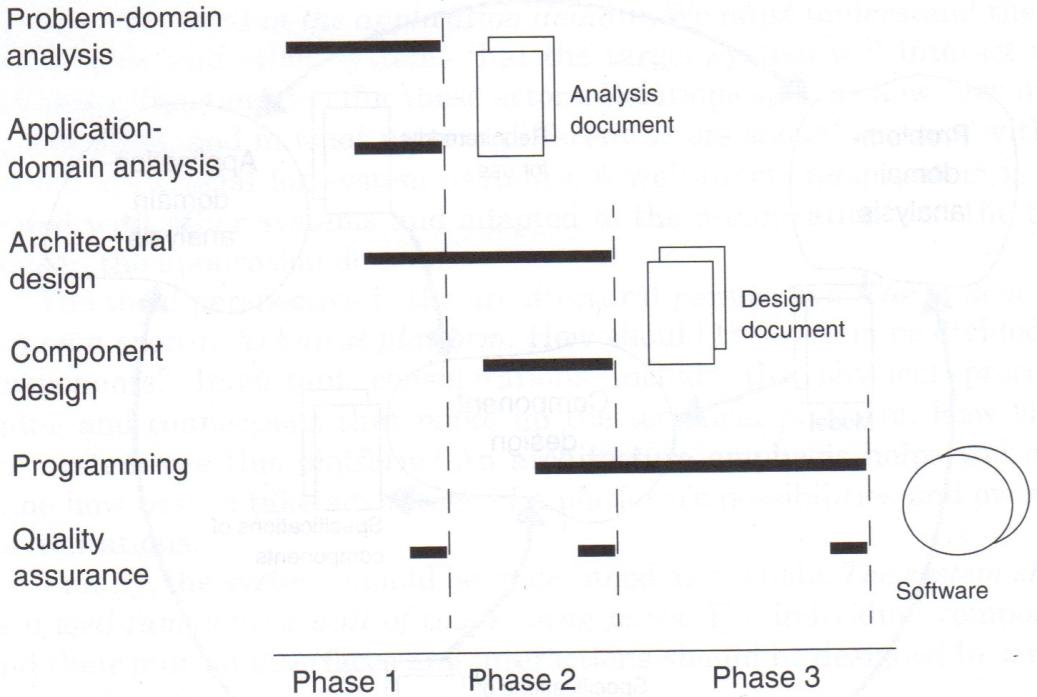
\includegraphics[width=\textwidth]{billeder/SUModel1.jpg}
		\caption{Traditional-top-down approach \citep[p.~16]{Rod-Aalborg}}
		\label{fig:SUModel1}
	\end{subfigure}
	\quad
	\begin{subfigure}[b]{0.48\textwidth}
		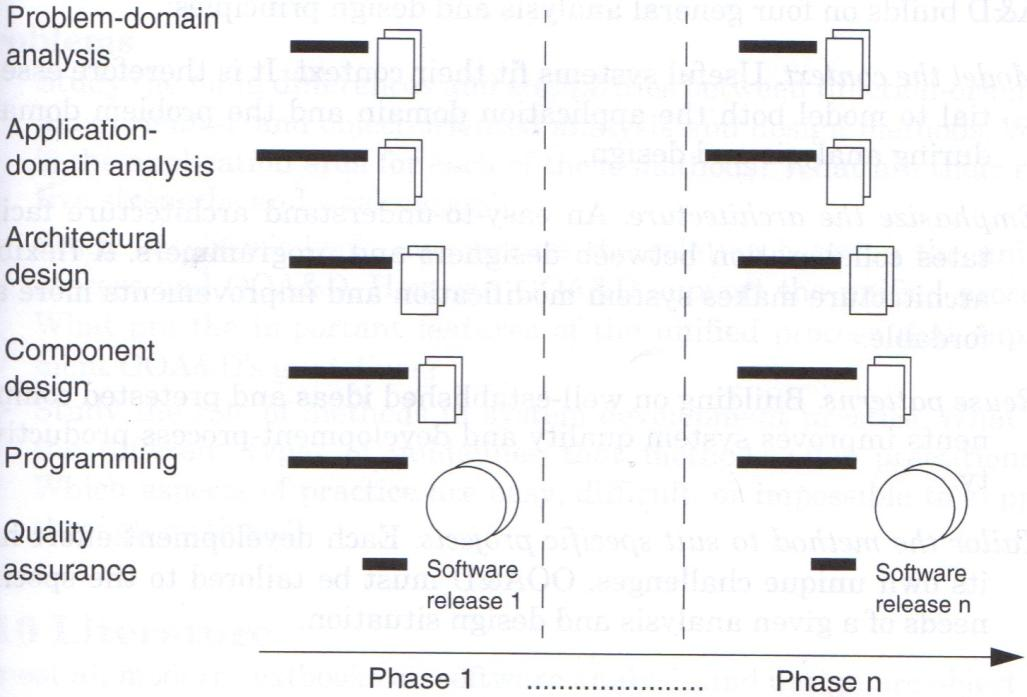
\includegraphics[width=0.9\textwidth]{billeder/SUModel2.jpg}
		\caption{Use-case driven, arcitecture-centric approach \citep[p.~17]{Rod-Aalborg}}
		\label{fig:SUModel2}
	\end{subfigure}
	\caption{Model based on the OOA\&D method}\label{fig:SUModels}
\end{figure}


\subsection{Using iterative life cycle in the project}
Throughout the project it is intended to design a system iteratively with a specific user’s needs and wants integrated into the designs and tests. This is the basis of choosing to work with the iterative model to reflect over which activity is being used throughout the stages of the project.
\section{First iteration}\label{sec:Iteration1}
\subsection{Simple timeline}\label{sec:1-simpleTime}
The first iteration started with a short presentation to the software development project through a mediator on Ipsen's behalf.
Right after this an initial interview to talk about the requirements was planned.

During the time up to the interview the workflow was in the understanding phase from \cref{fig:DEBModel}.
In this phase existing solutions was looked into and ideas generated, such that there was an opportunity to discuss unbiased, and through this also get Ipsen to reflect upon her requirements.
The interview was the start of the first evaluation phase in this iteration.
The ideas presented at this interview include among other an build-in editor such that everything about the handbooks would be managed in the system.
Though this was shut down fast since for that to be useful it would need to always keep up to date on how Microsoft's UI for eg. Word would look, since it otherwise would take too long to get used to every time it was necessary to change anything in the handbook.
The notification system which is one of the requirements stated in this report, was also one of these beforehand generated ideas presented at the first interview. 
Another idea was to make a Web Interface which would either be locally on the clients server or on the World Wide Web. This was first shot down, though through discussion it became clear that this was not impossible, since there was better opportunities with the notification system which was turned into a requirement.

After the first interview the analysis work started, leading the workflow back to the understanding activity yet again.
The analysis done during this phase was mainly done based on two basic activities from \cref{fig:SUModels}.
The problem domain analysis, which in this iteration focused on; Requirements, FACTOR, initial class diagram and the event table.
And some elements in the application domain analysis, which were; PACT and the actor table.
During this period another small second interview was held with Ipsen to evaluate the understanding of the vocabulary concerning the problem domain, to make sure the terminology was correct.
Right before the second interview which closed the first iteration and started the next one, a couple of prototypes were drawn up on paper and then afterwards turned into an interactive prototype, by programming, which could be presented at the second interview.
This combined both the envisionment and design activities from \cref{fig:DEBModel}.

The first iteration ended with the third interview, where the requirements in form of the FACTOR analysis was discussed and evaluated.
After this a couple of questions was asked clearing up confusion and misunderstandings surrounding the approval system, the role hierarchy and the supplier subsystem.
Lastly, the interactive prototype of this iteration was presented.
%Taniya: Hvad er det for noget interactive prototype der var presented - gætter på vores allerførste usability test (Lu's anden usability test)?
%Taniya: Hvornår er den første iteration sluttet? Efter den anden interview eller den tredje interview? 

\subsection{Elements to take notice of}
\subsubsection*{Class diagram}
During the first iteration the class diagram itself went through multiple developments.
It's final version can be seen in \cref{fig:ClassDiagram}.
In the first development, see \cref{fig:FirstClassDiagram}, the approval class was not seen as part of the main classes in the problem domain and therefore not present in the diagram.
Another difference in the first development was how the different roles was only thought of as attributes instead of classes in themselves and therefore were not present either.

\begin{figure}[H]
	\centering
	\begin{tikzpicture}[align=center, scale=1.0, transform shape]
	%De enkelte noder i diagrammet
		\node(hand)[process]{Handbook};
		\node(doc)[process, below=1cm of hand]{Document};
		\node(dep)[process, right=1.5cm of doc]{Notification};
		\node(ver)[process, below=1cm of doc]{Version};
		\node(read)[process, right=3cm of ver]{Read Status};
		\node(user)[process, right=2.1cm of hand]{User};
	%Linjer i billedet:
		\draw[{open diamond}-](hand.south)node[right, yshift=-0.2cm]{1}--(doc.north)node[left, yshift=0.2cm]{1..*};
		\draw[{open diamond}-](doc.south)node[right, yshift=-0.2cm]{1}--(ver.north)node[left, yshift=0.2cm]{0..*};
		\draw[black](doc.east)node[above, xshift=0.2cm]{1}--(dep.west)node[below, xshift=-0.35cm]{0..*};
		\draw[black](ver.east)node[above, xshift=0.2cm]{1}--(read.west)node[below, xshift=-0.35cm]{0..*};
		\draw[black](hand.east)node[above, xshift=0.2cm]{1}--(user.west)node[below, xshift=-0.35cm]{1..*};
		\draw[black](user.south)node[right, yshift=-0.2cm]{1}--(dep.north)node[left, yshift=0.2cm]{0..*};
		\draw[black](user.east)node[above, xshift=0.2cm]{1}-|(read.north)node[left, yshift=0.2cm]{0..*};
	\end{tikzpicture}
	\caption{First class diagram of developing process}\label{fig:FirstClassDiagram}
\end{figure}

Throughout the first iteration approval turned into a class in its own rights and therefore was cooperated into the diagram.
The role pattern came forth during this iteration as well though the final form of it went through a couple of evolutions.
The main discussion about this element was whether or not the reader class was necessary since all users by default was readers. 
Though it was decided for clarity to keep it.
%Anna: er ikke sikker på det her er nødvendigt og ikke bare bliver for meget.
%Another debate was revolved around the writer and why they were necessary. 
%Though it soon became clear through the second interview with Ipsen that this was not to be changed since there would be more Writers than administrators and it was good the writers did not have total access to the system the same way the administrator has.

\subsubsection*{Prototyping}
% Taniya: er det ikke fra anden interview? den prototype uden funktioner
The development of the prototype used in the third interview with Ipsen started out as drafted versions which can be found in \cref{sec:First-sketches,sec:Second-sketches}.
Based on these sketches an interactive prototype was made. 
Screenshots of some of the interfaces in this prototype can be found in \cref{sec:1prototype}.
The prototype did not have any of the system required functionality implemented.
It was used to let Ipsen move around and thereupon create a debate of whether or not the envisionment of the final system was correct or if something needed to be adjusted.
\section{Figure 1}
\begin{figure}[H]
	\centering
	\begin{tikzpicture}[align=center, scale=1.0, transform shape]
	%noder i billedet
		\node(start)[n]{};
		\node(main)[predefined, right=2.8cm of start]{Main page};
		\node(preview)[predefined, below=1.5cm of main]{Document\\ preview};
		\node(read)[predefined, right=3.2cm of preview]{Read status\\ overview pop-up};	
		\node(end)[n, above=1.5cm of read] {};
		\node(End)[c,fit=(end)] at (end) {};
	%Pile i billedet
		\draw[arrow](start.east) -- node [above]{login to\\ OBHandbooks} (main.west);
		\draw[arrow] (main.south) -- node [left]{Select\\ document}(preview.north);
		\draw[arrow](preview.east) -- node[below]{Press 'read status\\ overview'} (read.west);
		\draw[arrow](read.north) --node[left]{Press 'x'\\ to exit}(End) node[right=0.5cm]{};%{Close};
		%\draw[arrow](read.north west) -- node[above]{Press 'x'\\ to exit}(preview.north east);
	
	\end{tikzpicture}
	\caption{{\color{red}View who has read a document}}\label{fig:Use-ReadStatus}
\end{figure}

\section{Figure 2}
\begin{figure}[H]
	\centering
	\begin{tikzpicture}[align=center, scale=1.0, transform shape]
	%Noder i billedet
			\node(start)[n]{};
			\node(main)[predefined, right=2.8cm of start]{Main page};
			\node(new)[predefined, below=1.5cm of main, xshift=-2cm]{New file\\upload page};
			\node(preview)[predefined, right=2.5cm of new]{Document\\ preview};
			\node(doc)[predefined, below=1.5cm of new, xshift=-2cm]{Create\\new Document};
			\node(ver)[predefined, right=2cm of doc]{Create\\new version};
			\node(title)[predefined, below=1.5cm of doc]{Title \& ID\\checked};
			\node(upload)[predefined, right=2.8cm of title]{Upload\\file};
			\node(log)[predefined, right=3.5cm of upload]{Changelog\\created};
			\node(approve)[predefined, above=1.5cm of log]{Approval\\ created};
			\node(sent)[predefined, above =1.5cm of approve]{Approval request\\sent};
			\node(end)[n, above=1.5cm of sent] {};
			\node(End)[c,fit=(end)] at (end) {};
		%Streger i billedet
			\draw[arrow](start.east)--node [above]{login to\\ OBHandbooks}(main.west);
			%Ud fra main page
			\draw[black](main.south)--(4.01,-0.8);
			\draw[arrow](4.03,-0.8)-|node[right, yshift=-0.5cm]{Press\\'Upload'}(new.north);
			\draw[arrow](4.03,-0.8)-|node[left, yshift=-0.5cm]{Select\\document}(preview.north);
			%ud fra new file
			\draw[black](new.south)--(2.02,-3.3);
			\draw[arrow](2.02,-3.3)-|node[right, yshift=-0.5cm]{Add new\\ID}(doc);
			\draw[arrow](2.02,-3.3)-|node[left, yshift=-0.5cm]{Select\\existing ID}(ver);
			%Andre pile
			\draw[arrow](doc.south)--node[right]{Add\\title}(title.north);
			\draw[arrow](title.east)--node[above]{Select file}(upload.west);
			\draw[arrow](ver.south)--node[left]{Select\\file}(upload.north);
			\draw[arrow](preview.south)--node[right]{Press 'Upload\\new version'}(upload.north east);
			\draw[arrow](upload.east)--node[above]{Add changelog}(log.west);
			\draw[arrow](log.north)--node[left]{Add\\approvers}(approve.south);
			\draw[arrow](approve.north)--node[left]{Press ' send\\to approval}(sent.south);
			\draw[arrow](sent.north)--(End.south);
			\draw[black](sent.south east)|-(2.5,-8.15);
			\draw[black](2.5,-8.15)-|(-1.5,-4.0);
			\draw[arrow](-1.5,-4.0)|-node[above, xshift=1.0cm]{Invalid\\info}(new.west);
			\draw[arrow](upload.north east)--(approve.south west);
	\end{tikzpicture}
	\caption{{\color{red}Add new file to the system -suggestion}}\label{fig:Use-AddDoc}
\end{figure}

\section{Figure 3}
\begin{figure}[H]
	\centering
	\begin{tikzpicture}[align=center, scale=1.0, transform shape]
	%noder i billedet:
		\node(start)[n]{};
		\node(login)[predefined, right=2.8cm of start]{Login\\page};
		\node(main)[predefined, below=1.5cm of login]{Main page};
		\node(setting)[predefined, right=2.0cm of login]{Settings\\page};
		\node(info)[predefined, right=2.5cm of setting]{Information\\checked};
		\node(preview)[predefined, right=2.8cm of main]{Document\\preview};
		\node(end)[n, right=2.8cm of preview] {};
		\node(End)[c,fit=(end)] at (end) {};	
	%linjer i billedet:
		\draw[arrow](start.east)--node[above]{open\\OBHandbooks}(login.west);
		\draw[arrow](login.south)--node[left]{Normal\\login}(main.north);
		\draw[arrow](login.east)--node[above]{First time\\login}(setting.west);
		\draw[arrow](setting.north east)--node[above]{Fill out\\informations}(info.north west);
		\draw[arrow](info.west)--node[below]{invalid info}(setting.east);
		\draw[arrow](info.south west)--node[right, xshift=0.5cm]{Valid info}(main.north east);
		\draw[arrow](main.east)--node[below]{Select\\document}(preview.west);
		\draw[arrow](preview.east)--(End.west);
		%Loop arrows
		\path[arrow] (main) edge [loop below, looseness=7] node[auto] {Unfold a chapter} (main);
		\path[arrow] (main) edge [loop left, looseness=3] node[auto] {Unfold all\\chapters} (main);
		\path[arrow] (preview) edge [loop below,looseness=4] node[auto] {Download}(preview);
	
	\end{tikzpicture}
	\caption{{\color{red}Access current handbook}}\label{fig:Use-access}
\end{figure}

\section{Figure 4}
\begin{figure}[H]
	\centering
	\begin{tikzpicture}[align=center, scale=1.0, transform shape]
	%Noder i billedet
		\node(start)[n]{};
		\node(main)[predefined, right=2.8cm of start]{Main page};
		\node(dep)[predefined,right=2.8cm of main]{Department\\main page};
		\node(add)[predefined, below=1.5cm of dep]{Add name of\\new department};
		\node(detail)[predefined, left=4.5cm of add]{Detail view\\of department};
		\node(editD)[predefined, below=1.5cm of detail,xshift=1.5cm]{Manage documents\\in department page};
		\node(editU)[predefined, left=0.5cm of editD]{Manage users in\\department page};
		\node(delete)[predefined, right=2cm of editD]{Department\\deleted};
		\node(update)[predefined, below=1.5cm of editU, xshift=2cm]{Department\\updated};
		\node(end)[n, below=1.9cm of delete] {};
		\node(End)[c,fit=(end)] at (end) {};	
	%streger i billedet
		\draw[arrow](start)--node[above]{Login to\\OBHandbooks}(main);
		\draw[arrow](main)--node[above]{Go to\\'Departments'}(dep);
		\draw[arrow](dep)--node[left=0.9cm]{Select a\\department}(detail);
		\draw[arrow](dep)--node[right]{Add a new\\department}(add);
		\draw[arrow](add)--node[above]{New department's page}(detail);
		\draw[arrow](delete)--(End);
		\draw[arrow](update)--(End);
		%ud fra detail view
		\draw[black](detail.south)--(1.65,-3.5);
		\draw[arrow](1.65,-3.5)-|node[left=1cm, below]{Press 'edit\\documents'}(editD);
		\draw[arrow](1.65,-3.5)-|node[left=0.9cm, below]{Press 'edit\\users'}(editU);
		\draw[arrow](1.65,-3.5)-|node[left=1.1cm, below]{Press 'delete\\department'}(delete);
		%Ned til updated
		\draw[arrow](1.32,-6.0)--node[right]{Press\\'Apply list'}(update.north);
		\draw[black](editU)|-(1.32,-6.0);
		\draw[black](editD)|-(1.32,-6.0);
	%loops i billedet
		\path[arrow] (editU) edge [loop left, out=208, in=190, looseness=4] node[below] {Add/remove\\documents} (editU);
		\path[arrow] (editD) edge [loop right,out=335, in=350, looseness=4] node[below] {Add/remove\\users} (editD);
	\end{tikzpicture}
	\caption{{\color{red}Manage departments}}\label{fig:Use-dep}
\end{figure}

\section{Figure 5}
\begin{figure}[H]
	\centering
	\begin{tikzpicture}[align=center, scale=1.0, transform shape]
	%noder i billedet
	\node(start)[n]{};
	\node(main)[predefined, right=2.7cm of start]{Main\\page};
	\node(user)[predefined,right=2.6cm of main]{User management\\page};
	\node(delete)[predefined, right=1.6cm of user]{User\\deleted};
	\node(end)[n, below=2cm of delete] {};
	\node(End)[c,fit=(end)] at (end) {};
	
	\node(update)[predefined, left=2.8cm of End]{User\\updated};
	\node(edit)[predefined, left=2.8cm of update]{Edit user\\page};	
	%streger i billedet
	\draw[arrow](start)--node[above]{Login to\\OBHandbooks}(main);
	\draw[arrow](main)--node[above]{Go to 'User\\management'}(user);
	\draw[arrow](user)--node[above]{Press\\'Delete'}(delete);
	\draw[arrow](delete.south)--(End.north);
	\draw[arrow](update.east)--(End.west);
	\draw[arrow](edit.east)--node[above]{press 'save'}(update.west);
	\draw[arrow](edit.north east)--node[right=1.4cm]{Press\\'Delete'}(delete.south west);
	\draw[arrow](user.south west)--node[left=0.4cm]{Select a\\user}(edit.north);
	%loop i billedet
	\path[arrow] (edit) edge [loop left, looseness=3] node[left] {Change\\information} (edit);
	%Anna: Det er den linje her nedenfor som todo'en omhandler
	\path[arrow] (edit) edge [loop below, looseness=4] node[below] {Change\\password} (edit);
	
	\end{tikzpicture}
	\caption{{\color{red}User management}}\label{fig:Use-userman}
\end{figure}
\todo[inline]{Anna tanke: burde man evt bare fjerne den med password hvis vi holder det som på den måde det er i systemet nu, da det hele foregår i samme omgang,og så bare har den der hedder update system}

\section{Figure 6}
\begin{figure}[H]
	\centering
	\begin{tikzpicture}[align=center, scale=1.0, transform shape]
	%noder i billedet
		\node(start)[n]{};
		\node(main)[predefined, right=2.7cm of start]{Main page};
		\node(profile)[predefined, right=1.8cm of main]{User setting\\page};
		\node(update)[predefined, below=1.5cm of profile]{Profile\\updated};
		\node(end)[n, left=2.8cm of update] {};
		\node(End)[c,fit=(end)] at (end) {};	
	%streger i billedet
		\draw[arrow](start.east)--node[above]{Login to\\OBHandbooks}(main.west);
		\draw[arrow] (main.east)--node[above]{Press the\\cogwheel}(profile.west);
		\draw[arrow] (profile.south)--node[left]{Press\\'save'}(update.north);
		\draw[arrow] (update.west)--(End.east);
	%loop i billedet
		\path[arrow] (profile) edge [loop right, looseness=3]node[auto]{Change\\information} (profile);	
	\end{tikzpicture}
	\caption{{\color{red}Edit user information}}\label{fig:Use-profile}
\end{figure}

\section{Figure 7}
\begin{figure}[H]
	\centering
	\begin{tikzpicture}[align=center, scale=1.0, transform shape]
	%noder i billedet
		\node(start)[n]{};
		\node(main)[predefined, right=2.7cm of start]{Main page};
		\node(archive)[predefined, right=1.8cm of main]{Archive page};
		\node(download)[predefined, below=1.5cm of archive]{Downloaded\\archive};
		\node(ver)[predefined, left=2.8cm of download]{Version\\page};
		\node(end)[n, below=0.8cm of ver, xshift=2cm]{};
		\node(End)[c, fit=(end)] at (end){};
	%streger i billedet
		\draw[arrow](start.east)--node[above]{Login to\\OBHandbooks}(main.west);
		\draw[arrow](main.east)--node[above]{Go to\\'Archive'}(archive.west);
		\draw[arrow](archive.south)--node[right]{Press\\'Download}(download.north);
		\draw[arrow](archive.south west)--node[left=0.6cm]{Selct a\\version}(ver.north east);
		\draw[arrow](5.23,-3.1)--(End.north);
		\draw[black](ver.south)|-(5.25,-3.1);
		\draw[black](download.south)|-(5.25,-3.1);
	%loop i billedet
		\path[arrow] (archive) edge [loop right, in=355, looseness=3]node[auto]{Unfold\\documents} (archive);
		\path[arrow] (archive) edge [loop above, in=65, looseness=6]node[auto]{Unfold\\chapters} (archive);
		\path[arrow] (ver) edge [loop left, looseness=4]node[auto]{Download\\version} (ver);
	
	\end{tikzpicture}
	\caption{{\color{red}Access Archive}}\label{fig:Use-archive}
\end{figure}

\section{Figure 8}
\begin{figure}[H]
	\centering
	\begin{tikzpicture}[align=center, scale=1.0, transform shape]
	%noder i billedet
		\node(start)[n]{};
		\node(main)[predefined, right=2.7cm of start]{Main page};
		\node(user)[predefined, right=2.8cm of main]{User management\\page};
		\node(create)[predefined, below=1.5cm of user]{Create user\\page};
		\node(update)[predefined, left=1.5cm of create]{User\\created};
		\node(end)[n, left=1.5cm of update]{};
		\node(End)[c, fit=(end)] at (end){};
	%streger i billedet
		\draw[arrow](start.east)--node[above]{Login to\\OBHandbooks}(main.west);
		\draw[arrow](main.east)--node[above]{Go to 'User\\administration'}(user.west);
		\draw[arrow](user.south)--node[right]{Press\\'Create user'}(create.north);
		\draw[arrow](create.west)--node[above]{Press\\'save'}(update.east);
		\draw[arrow](update.west)--(End.east);
	%loop i billedet
		\path[arrow](create) edge [loop below, in=255, looseness=4]node[auto]{Add\\information} (create);
		\path[arrow](create) edge [loop below, out=345, in=320, looseness=3] node[right]{Add\\departments} (create);
			
	\end{tikzpicture}
	\caption{{\color{red}Add user}}\label{fig:Use-AddUser}
\end{figure}

\todo[inline]{Anna kommenterer: hver opmærksom på at der eksplicit netop i ideen var at man skal kunne tilføje departments under user-creation (hvilket på givne tidpunkt ikkeer implementeret)}

\section{Figure 9}
\begin{figure}[H]
	\centering
	\begin{tikzpicture}[align=center, scale=1.0, transform shape]
	%noder i billedet
		\node(start)[n]{};
		\node(main)[predefined, right=2.7cm of start]{Main page};
		\node(pending)[predefined, right=3.0cm of main]{Pending\\approval page};
		\node(approve)[predefined, below=1.5cm of pending]{Pending approval\\approved};
		\node(ver)[predefined, left=2.8cm of approve]{pending approval\\verison page};
		\node(active)[predefined, below=1.5cm of approve]{Version active\\in handbook};
		\node(end)[n, left=1.5cm of active]{};
		\node(End)[c, fit=(end)] at (end){};
	%streger i billedet
		\draw[arrow](start.east)--node[above]{Login to\\OBHandbooks}(main.west);
		\draw[arrow](main.east)--node[above]{Admin:Go to\\Pending approval}(pending.west);
		\draw[arrow](pending.south)--node[right]{Press\\'Approve'}(approve.north);
		\draw[arrow](main.south)--node[left]{Writer: go through\\notifications}(ver.north);
		\draw[arrow](pending.south west)--node[left, yshift=0.28cm]{Select an\\ approval}(ver.north east);
		\draw[arrow](ver.east)--node[above, xshift=0.45cm]{Press\\'Approve'}(approve.west);
		\draw[arrow](approve.south)--node[right]{Version approved\\by all approvers}(active.north);
		\draw[arrow](approve.south west)--node[left]{Admin unilateraly\\approves version}(active.north west);
		\draw[arrow](active.west)--(End.east);
		
	\end{tikzpicture}
	\caption{{\color{red}Approve new version}}\label{fig:Use-ApproveVer}
\end{figure}
\todo[inline]{Anna kommentar: i teksten til pilen main page til pending approval version page hvor der står "Writer: go through\\notifications" stod der oprindegligt "Press notification button", så hvis hellere vil have det, bare ændre det}

\section{Figure 10}
\begin{figure}[H]
	\centering
	\begin{tikzpicture}[align=center, scale=1.0, transform shape]
	%noder i billedet
		\node(start)[n]{};
		\node(main)[predefined, right=2.7cm of start]{Main page};
		\node(status)[predefined, right=2.8cm of main]{Document\\preview};
		\node(pop)[predefined, below=1.5cm of status]{Pop-up menu};
		\node(update)[predefined, left=2.5cm of pop]{Read status\\updated};
		\node(end)[n, left=1.5cm of update]{};
		\node(End)[c, fit=(end)]at (end){};
	%streger i billedet
		\draw[arrow](start.east)--node[above]{Login to\\OBHandbooks}(main.west);
		\draw[arrow](main.north east)--node[above]{Go through\\notifications}(status.north west);
		\draw[arrow](main.east)--node[below]{Select relevant\\document}(status.west);
		\draw[arrow](status.south)--node[left, yshift=-0.2cm]{Press\\'Read status'}(pop.north);
		\draw[arrow](pop.west)--node[below]{Press 'Agree'}(update.east);
		\draw[arrow](update.west)--(End.east);
	%loop i billedet
		\path[arrow](pop) edge [loop right, looseness=1]node[right]{Press\\'Cancel'} (status);	
	
	
	\end{tikzpicture}
	\caption{{\color{red}Mark document as read}}\label{fig:Use-Read}
\end{figure}

\todo[inline]{Anna kommentarer:Vær opmærksom på jeg har ændret en del pile i diagrammet \\husk kun writer og reader kan det her.\\ Husk som det ser ud i implementationen i dag er det ikke et pop-up vindue}
%\section{Second iteration}
\subsection{Simple timeline}\label{sec:2Iteration-timeline}
After the third interview with Ipsen the second iteration started with the evaluation activity from \cref{fig:DEBModel}. 
During this activity the data gathered at the interview was reevaluated and used to update the relevant models and analysises such as the FACTOR model and the class diagram.
During the interview the first signs of the iterative model being the right model to work with became clear.
%Since Ipsen had changed her decision upon how the archive should work.
During the small second interview in iteration 1, it was said that the date search function in the archive would be obsolete.
However when it was presented as a part of the protoype the possible usage became clearer and it was turned into a requirement.
%fjernet nedenunder erstattet ovenover.
%But when it was a part of the prototype and therefore clearer illustrated it turned into a requirement.
%virker underligt at vi har inkluderet det i en prototype hvis det allerede var blevet affejet som obsolete

After the evaluation activity an understanding phase started where the first analysis of the functions in the application domain activity was done as well as the development of rich picture analysis in the problem domain activity, \cref{fig:RP-Oversigt,fig:RoleIllustration}.
Hereafter, the architectural design was reevaluated from the first rough ideas in iteration 1, and the development of component design started.
Leading the workflow into a mix of the understanding and design activities. 
See \cref{fig:DEBModel,fig:SUModels}.

During this iteration a design process concerning the interface design began, using a mix of envisionment and design activities from \cref{fig:DEBModel}.
The prototype presented at the third interview was during this period further developed and implemented with some of the required functionalities.

The second iteration ended with at usability test with Ipsen based upon the iterated prototype. 
At the end of the meeting with Ipsen the designs of the interfaces were presented and shortly discussed to clarify whether or not the differences between reader, writer and administrator were correctly understood.

\subsection{Elements to take notice of}
\subsubsection*{Supplier sub-problem} 
The general idea of the supplier sub-problem was presented by Ipsen during the initial interview in the first iteration as an impulsive thought.
In the course of the first iteration there was an awareness of the sub-problem but it quickly became clear through the discussions in the analysis that more information was needed to completely analyze it and its role in the problem domain.

At the third interview the supplier sub-problem was discussed through a series of questions prepared beforehand to resolve the needed information.
Afterwards in the second iteration, the problem domain analysis was as mentioned in \cref{sec:2Iteration-timeline}. 
% Taniya: was mentioned and . . . ? føler at der mangler noget her? 
This was done especially with the focus on in-cooperating the supplier subproblem.
This meant changes to the FACTOR analysis and the class diagram.
As for the class diagram the introduction of the supplier and later the refinement of the approval classes led to the final draft seen in \cref{fig:ClassDiagram}.
%forkert figurreference. det her er den første ikke den sidste - astrid

\subsubsection*{FACTOR}
In addition to the supplier subproblem mentioned above the FACTOR analysis went through two significant changes during the second iteration.

The first change is the role hierarchy which was turned from four levels into three.
% Taniya:  four levels into four?
During the first iteration it had become unclear whether or not a fourth level was needed in the role hierarchy.
In the original FACTOR it was written as follows
\footnote{Note: The writing style was more detailed in the first FACTOR to make sure the requirements was understood correctly, when the second interview came around.}:
\newline
''Different levels of permissions/access rights to the documents within the handbook
\begin{itemize}
	\item 
	0 level:
	Reading the handbook except secured documents
	\item 
	1st level:
	Reading the whole handbook
	\item 
	2nd level:
	Editing selected documents
	\item 
	3rd level:
	Total access to editing documents and access to archive''
\end{itemize}

Though it was concluded from the third interview that only three roles were needed, as confidential documents usually are not included in the handbook.
These are mentioned in the FACTOR analysis found in \cref{factor}.

The second significant difference is how most of the functionality and some of the conditions from the FACTOR analysis has turned into requirements in the MoSCoW presented in \cref{sec:requirementsdefinition}. 
These are among other ''The handbook should be printable'' and ''Title and chapter number are linked. If a title is removed the chapter number cannot be used for anything else.'', from the FACTOR analysis draft in iteration 1.

\subsubsection*{Event table}
The event table went through quite an evolution throughout the second iteration.
Some of these evolutions will be presented in the following.

One of the larger discussions about the event table is the 'user deactivated' and 'user reactivated' vs. 'user deleted' points discussed in \cref{sec:Events}.
During this iteration it was decided to not use deactivated and reactivated since the use case for it would be such a rare case.
Furthermore, the delete user was discussed and a solution of how to save read status' without too much user information was found.
The main problem for this and the main reason for this debate, is due to not wanting to save unnecessary information and through this way get in trouble with the general data protection regulation (GDPR).
%eftetrsom vi aldrig bruger denne forkortelse igen dø den
This is not something that will be further discussed though.

Another change from first to second iterations how the supplier sub-problem has become a part of the event table.
As mentioned before the third interview cleared up questions about this sub-problem and it could become part of the system design and analysis.

Further developments to the event table is how the events 'subscribed to documents' and 'unsubscribed' was reevaluated as the idea of departments got more worked out.
These events turned into the department block of events in the table found in \cref{fig:eventtable};
\begin{itemize}
	\item 
	Department added
	\item
	Department's users updated
	\item
	Department's documents updated
	\item
	Department deleted
	\item
	Department notified user
\end{itemize} 

Finally, the event table was also filled out with the markings connecting the different classes and events and how many times the event occurs.
%Taniya: how many times the event could occur? istedet for måske? det lyder som om vi skriver præcis hvor mange gange events vil ske?

\subsubsection*{Some conclusions on last prototype}
As written in \cref{sec:2Iteration-timeline}, one conclusion from the end of the first iteration, is the need of the date search function in the archive, seen in \cref{fig:3-archive}.
The reason for the turn around decision on this point is Ipsen's realization of how it would make audits easier.
Due to the need sometimes arising, of finding all documents and versions active throughout at given period.

Another conclusion is how the notification system was not meant to be as extensive as first understood. 
This became clear with the debate on the need for marking if a version included 'minor' or 'major' changes, seen in \cref{fig:3-UploadVer}.
The result of this debate being no since the company, the system is meant for, is so small that if it were major changes an oral notice would suffice.
It became further clear when it was decided that it should not be possible to deny approvals, \cref{fig:3-ApproveDenied}, since the client would discuss such things outside the system.
%Taniya: er client det rette ord?

\subsubsection*{Further prototype development}
At the fourth meeting with Ipsen which ended the second iteration a further developed functional prototype, based on the one from the first third interview was presented in a usability test, \cref{secondtest}.
%Taniya:  ..the first third interview? det er vel third interview?
The development was done iterativly in accordance with the chosen method in such a way that new functionality was added to the code of the first prototype.
Screenshots of some of the interfaces in this prototype can be found in \cref{sec:2prototype}.
%Taniya: screenshots er ikke blevet tilføjet i appendix

During the second iteration the beginning of designing a mock-up of the whole system, starting with the reader and writer view, was done. 
These designs can be found in \cref{sec:Mock}.

%\section{Third iteration}
\subsection{Simple timeline}\label{sec:3Iteration-timeline}
The third iteration started with the evaluation activity from \cref{fig:DEBModel} based upon the fifth meeting with Ipsen, where the interactive prototype, with added functionality, and the mock-up design were presented.
%Taniya? 5 meeting er det ikke den sidste møde/usability test vi har med Pia? og hvad er det for nolge mock-up design blev der fremvist til Pia? Eller mener du den 4 meeting? 
At the end of the evaluation activity the work proccess flowed into a combination of the design and envisionment activities as well as the understanding activity.
The combination of design and activity was mainly used when further developing the mock-up.
As for the understanding activity, this was used mainly in combination with the evaluation activity when revisiting the analysis and design of the system.

During the iteration the class diagram belonging to the problem domain in \cref{fig:SUModels} was evolved to its final evolution presented in this report, see \cref{fig:ClassDiagramNoSupplier}.
This diagram indicating the actual sub-problem being in focus of this report.
The workflow also went through the application domain activity seen in.
%Taniya: det ser ud til at der mangler noget \cref{}
During this process, the function list, actors and use cases were revisited.
Furthermore the third iteration also included a visit to the architectual design and component design activities.
Until this point these activities had been shortly discussed and sketched.
Though in this iteration the elements in these activities were more thoroughly designed and worked upon.
Leading to the results seen in \cref{sec:architecturecriteria,sec:AppMethod,sec:componentdesign}.
Parallel with this workflow the design process on the Mock-up continued.

Iteration three ended with a usability test done with Ipsen and her immediate family as test subjects.
Followed by a short discussion with Ipsen about the system in general.
This iteration was meant to end with another usability test done two days after the one with Ipsen and her family though because of some complications this was not held.

\subsection{Elements to take notice of}
\subsubsection*{Actors and use-cases}
The larger element to take notice of which will be mentioned is that of the actors and use cases from the application domain.
In this iteration the actors was turned from:
\begin{itemize}
	\item
	Consultant
	\item
	Secretary
	\item
	Manager
	\item
	Worker
	\item
	Software
\end{itemize}

Into those found in \cref{tab:ActorTable} which are 'Administrator', 'Writer' and 'Reader'. 
% Henrik er lidt forvirret her
Instead the relevant specific cases that existed to begin with was turned into examples in the different actor tables in \cref{sec:Actors}.

As for the use cases they also evolved quite a bit in this iteration.
The following paragraphs will first present the original use-case names followed by a description of the changes done in this iteration.
%Taniya: use-case med bindestreg?

\textbf{Manage documents} was turned into three more specific cases such that there would be no question about what was included in the use-case.
These new cases which are those used in this report are \textit{Access current handbook}, \textit{Add new file to the system} and \textit{Access archive}.

\textbf{Manage users} was in the same way turned into more specific cases.
These being \textit{Add user} and \textit{User management}.
Furthermore, the use-case \textit{Edit user information} was added to the table.
The reason for this being that the other two cases are features meant for the administrator role, while this last one is meant for one to change his own information.

\textbf{Read status} is a feature meant to help keep track of who has read the document among those that need to.
The use-case was divided into two since it includes two angles.
The first angle being the one for those that need to be kept track of and the last, the one for those who are keeping track.
These more specified use-cases is respecitvly called \textit{View who has read a document} and \textit{Mark document as read}.

Other than these, aforementioned three use-cases, two were renamed but otherwise kept the same and three other cases was removed.
Those that were removed were \textit{Update TOC}, \textit{Track differences} and \textit{Manage suppliers}.
The first one about the TOC was removed since this was not a use-case relevant for the application domain after 'software' was removed from among the actors.
The use-case about tracking differences was removed for two reasons.
One being the same as the one for the TOC use-case.
The other reasons was that this case was evaluated to a nice to have requirement that in no way was necessary for the work.
Furthermore, before it could be useful and not obstructing the users workflow it would need a rather huge analysis and design process in itself.
Lastly, the supplier use-case was removed since the sub-problem concerning this use-case was scoped out in the problem domain analysis.

\subsubsection*{Some conclusions on last prototypes}
At the end of the second iteration a usability test was held with Ipsen based upon the functional prototype available at that point in time, \cref{secondtest}.
One specific note worth specifically mentioning in this section is how the issue with the negative ID numbers, which is described in more details in \cref{secondtest}, caused for the document class to be reevaluated.
%Taniya: Hvordan reevaluated?
Thereby, leading the class into another iteration concerning its design.
The results of the evaluation being that it should be possible to delete a document if a file have not yet been attached and approved.

The last thing that will be mentioned here as well is how Ipsen when interacting with the archive found it weird that the active version of a document would be present as well.
Though, shortly after, in the discussion it became clear that it was a likable feature that yet again would be helpful during audits, as well as when wanting to retrieve the whole handbook.

At this meeting with Ipsen, the Mock-up which had been designed until then was also presented.
This was done to grant a visual of how the interface for writer and reader was understood and if this understanding was correct.
The conclusion of this came quickly and turned out positive.
For further detail on this test see \cref{thirdtest}.


\subsubsection*{Further prototype development}
During the third iteration the mock-up was further developed, now mainly focusing upon the administrators interfaces.
The main designs among these can be found in \cref{sec:2Mock}.

Lastly, the prototype from the end of the second iteration was further developed and implemented as well.
This new prototype was then used in the usability tests with Ipsen and her family, \cref{fourthtest}.
Some interfaces connected to the prototype at that point can be found in \cref{sec:3prototype}\footnote{Please note that the pictures used here does not include the actual documents used at the usability test due to confidentiality issues.}.
%Taniya: mangler at tilføje billeder i appendix 
After the test the prototype and the results was evaluated and some of the bugs fixed.
Which is the status for the program where this reports ends.

\chapter{Implementation}
This chapter will cover the implementation of the system. Introduction introduction, bla bla bla
\section{Directory structure}
The project, in it's essence, is divided up into \texttt{OBHandbooks} and \texttt{OBHandbooks.Tests}. Besides these, there are a series of utility shell scripts in the root dir used to restore backups and check the syntax.
\todo[inline]{Den her fætter skal lige deles op før vi afleverer}
%Anna kunne det være værd at sætte den i appendiks?
\dirtree{%
.1 /.
.2 OBHandbooks.Tests/.
.3 OBHandbooks.Tests.csproj.
.2 .github/.
.3 workflows.
.4 main.yml.
.2 /OBHandbooks/.
.3 Properties.
.4 launchSettings.json.
.3 Views.
.4 Approval/.
.4 Archive/.
.4 Document/.
.4 ReadStatus/.
.4 Account/.
.4 Admin/.
.4 Shared/.
.5 Components/.
.4 Version/.
.4 Settings/.
.4 Department/.
.3 Controllers/.
.3 wwwroot/.
.3 ViewModels.
.3 libman.json.
.3 ViewComponents.
.3 Models.
.3 OBHandbooks.csproj.
.3 appsettings.json.
.3 Infrastructure.
.3 appsettings.Development.json.
.3 Data.
.3 Repositories.
}

%Anna. Er der en grund til vi kun har en unflded og hvorfor lige den?
As can be seen, the project is split up into Views, Controllers, Models, Infrastructure, and Repositories.

The role of the Models, Views, and Controllers are as in a traditional MVC model.

\section{Code examples}
In this section examples of the code will be presented.
As written in \cref{sec:systemdesign} the system is based on the ASP.NET Core MVC architecture including EF Core.
How the system utilizes the MVC architecture and the EF Core framework will be shown in the following code examples.

Firstly the MVC implementation is explored with the Document class.
How the Document object is being treated throughout the system will be presented throught the model, view, and controller components.
Furthermore it will be shown how the document data will be stored in the database with the repository pattern and EF Core.
Here it will be shown in part how a new document is added into the system throughout the components.

\subsection{Model}

In the model component it Document object is defined.
As it is primarily the document object that will be highlighted in the code examples, how the document object is presented in the code snippet below:
\\
\begin{lstlisting}
[Key]
public int ID { get; set; } //for the database

public virtual Chapter Chapter { get; set; } //first part of document ID

public int ChapterNumber
{
	get
	{
		return Chapter != null ? Chapter.Number : -1;
	}
}

[Range(1, Int32.MaxValue)]
[Display(Name = "Section")]
public int SectionNumber { get; set; } //second part of Document ID

[Required]
public string Title { get; set; } // TODO: Unique title of document

public virtual ICollection<Version> Versions { get; set; } //List of all past versions of the document (the "archive")
public virtual IEnumerable<DocumentDepartment> DocumentDepartments { get; set; }

public bool Archived { get; set; }

public Document()
{
	Archived = false;
}
\end{lstlisting}

The document object includes an ID, chapter, chapter number, section number, section number, versions, and whether or not it has been archived as seen in the code snippet above.
The \texttt{key} attribute on line 1 specifies that the \texttt{int ID} is a key that the database can use to identify the specific document.
Likewise the \texttt{Range} attribute specifies that the section number is included in a an \texttt{enumerable} class consisting of integers from 1 to infinity.
And the \texttt{Display} attribute on line 15 specifies that the section number should be displayed with the name \textit{section}.
This \texttt{display} attribute is used with ASP.NET Core and is used to modify the text on the screen when a controller is rendered to the view.

In the code snippet below it is shown the logic of how a new version of a document is added.
\\

\begin{lstlisting}
public void AddVersion(Version version)
{
	version.ValidFromDate = DateTime.Now;
	version.Approved = true;
	Versions.Add(version);
	int nVersions = Versions.Count;
	var oldVersion = Versions.ElementAtOrDefault(nVersions - 1);

	if (nVersions >= 2 && oldVersion != null)
	{
		oldVersion.ValidUntilDate = DateTime.Now;
	}
	foreach (DocumentDepartment dd in DocumentDepartments)
	{
		dd.Department.Notify("The document " + Title + " has been updated", "http://localhost:5000/document/" + Chapter.Number.ToString() + "." + SectionNumber.ToString());
	}
}
\end{lstlisting}

As is seen on line 3 and 4 when a new version of a document is added it receives a new date from which is it valid and that the \texttt{Approved} bool is set to \texttt{true}.
On line 5 the new version is added to the list of versions.
The control sequence from line 9 - 12 ensures that the previous version's date is set to the day that it has been replaced by the new version.
When a new version has been added all of the affected department in the system will get notified as seen in the loop from line 13 - 16.

\subsection{Controller}

In the code examples below it is shown how a \texttt{HttpGet} and \texttt{HttpPost} methods are implemented in the controller component.
Firstly it is shown how the document object is arranged so that it can be rendered to the view through the \texttt{HttpGet} method.
\\

\begin{lstlisting}
[HttpGet("")]
[HttpGet("document/")]
public async Task<IActionResult> Index()
{
	var user = await this._userManager.GetUserAsync(HttpContext.User);
	var documentIndex = new ViewModels.DocumentIndex();
	foreach (var ud in user.UserDepartments)
	{
		foreach (var dd in ud.Department.DocumentDepartments)
		{
			if (!dd.Document.Archived) documentIndex.AssignedDocuments.Add(dd.Document);
		}
	}
	List<Document> documentList = await this._documentRepository.ListNonArchivedAsync();
	foreach (var d in documentIndex.AssignedDocuments)
	{
		documentList.Remove(d);
	}

	foreach (var d in documentList)
	{
		if (!documentIndex.UnassignedDocuments.ContainsKey(d.Chapter))
		documentIndex.UnassignedDocuments[d.Chapter] = new List<Document>();
		documentIndex.UnassignedDocuments[d.Chapter].Add(d);
	}

	@ViewData["Title"] = "Table of Contents";

	return View(documentIndex);
}
\end{lstlisting}

The \texttt{HttpGet} method means that the view component retrieves data from the controller.
Something to take not of is the \texttt{async Task<IActionResult>} on line 3.
The \texttt{Task} class represents a single operation \cite{microsoft}.
This operation does not return a value and usually executes asynchronously.
The \texttt{IActionResult} result method ensures that the controller returns a model to the view.

From line 5 - 13 it is determined which documents that the current user is assigned to.
This is done by first retrieving the current user, which is defined through \texttt{HttpContext.User}, by finding a match in the list of users found in \texttt{_userManager}.
Afterwards program sorts through the departments that the user is a part of to find which documents that the user is assigned to.
This is done through the loop from line 9 - 12.

After the user's assigned documents has been sorted a list of all the non-archived documents will occur in the view.
This is done through the two loops from line 14 - 25.
All of the non-archived documents are returned to the view through \texttt{var documentIndex} on line 29.

In the code snippet below it is shown what happens when the user adds a new document or versionto the system through the \texttt{HttpPost} method.
\\
\begin{lstlisting}
[HttpPost("document/add/")]
public async Task<IActionResult> Add(Document document,
	int chapterNumber,
	IFormFile versionFile,
	IFormFile workingFile,
	string requireApprovalCheck,
	string approvers)
{
	bool requireApproval = (requireApprovalCheck == "on");
	@ViewData["Title"] = "New document";
	@ViewBag.Chapters = await _chapterRepository.GetChapters();

	if (ModelState.IsValid)
	{
		document = this._documentRepository.ToProxy(document);
		var chapter = await this._chapterRepository.GetChapter(chapterNumber);

		if (chapter == null)
		{
			ModelState.AddModelError(string.Empty, "Problem happend getting the chapter.");

			return View(document);
		}

		document.Chapter = chapter;

		try
		{
			document = await this._documentRepository.AddAsync(document);
		}
		catch (DocumentAddException e)
		{
			ModelState.AddModelError(string.Empty, e.ModelError);
			return View(document);
		}
		if (versionFile != null)
		{
			OBHandbooks.Models.Version version = new OBHandbooks.Models.Version();
			version.SetDocument(document);
			version = await this._versionRepository.AddAsync(version);

			version.VersionFile = new HandbookFile(versionFile);
			if (workingFile != null) version.WorkingFile = new HandbookFile(workingFile);

			if (requireApproval)
			{
				HandbookApproval approval = await CreateApproval(
				approvers,
				await this._userManager.GetUserAsync(HttpContext.User));
				approval.DocumentVersion = version;
				version.DateSubmittedToApproval = DateTime.Now;
				document.Versions.Add(version);
				approval.CheckForApproval();
				await this._approvalRepository.UpdateAsync(approval);
			}
			else
			{
				document.AddVersion(version);
			}
			await this._documentRepository.UpdateAsync(document);
			await this._versionRepository.UpdateAsync(version);
		}
		return RedirectToAction(nameof(Index));

	}

	return View(document);
}
\end{lstlisting}

As the \texttt{HttpGet} method retrieves data from the controller, the \texttt{HttpPost} method ensures that new data is submitted into the controller and into the components further down the layers.

The information from the view is transfered into the controller method through the parameters shown from line 2 - 7.
When the document is posted to the controller the \texttt{Add} method ensures that the new document version needs to be approved line 9.
Afterwards the actual document receives its chapter number on line 16 and is saved into the document repository on line 29 through the \texttt{AddAsync} method.

The new version of the document is stored into the repository from line 36 - 62.
Here the new version is saved into the version repository on line 40 with the \texttt{AddAsync} method.
Notice that the \texttt{_documentRepository.AddAsync} and \texttt{_versionRepository.AddAsync} are similarly named, but saves a document and a version respectively.

The new document version is not yet valid to the readers as it needs to be approved.
From line 45 - 55 the program creates an approval object or objects where it is determined which users need to approve the new version.
If the new version does not need an approval, it is simply saved into the repositories on line 60 - 61.

\subsection{View}

\begin{lstlisting}
@foreach (KeyValuePair<Models.Chapter, List<Models.Document>> kvp in Model.UnassignedDocuments) {
<button class="btn btn-outline-dark text-left pl-4 mt-1" onclick="listExpand()" style="width: 100%; margin-top: 10px;" type="button" data-toggle="collapse" data-target="#collapseChapter-@kvp.Key.Number" aria-expanded="false" aria-controls="collapseExample">
<div class="row">
	@kvp.Key.Number | @kvp.Key.Name
	<i class="fas fa-chevron-down ml-auto mr-4 arrow-toggle"></i>
</div>
</button>
<div class="collapse card" id="collapseChapter-@kvp.Key.Number">
	<div class="card-body" style="padding: 0.1rem">
		<table class="table table-striped table-sm">
			<thead class="border font-weight-bold">
				<tr>
					<td>ID</td>
					<td>Title</td>
					<td>Version</td>
					<td>Date</td>
					<td>Read status</td>
					@if (User.IsInRole("Administrator"))
					{
						<td></td>
					}
				</tr>
			</thead>
		<tbody>
			@await Html.PartialAsync("_DocumentListBody", @kvp.Value)
		</tbody>
		</table>
	</div>
</div>
}

\end{lstlisting}
This is the view that represents a list of assigned documents. This will render to a button, which when clicked expands a list of documetns in the chapter the button represents.
It's written in the razor templating langugae, which is HTML, but with the added feature of allowing the documents to be dynamic when prefacing a statement with the \texttt{@} character.
An interesting thing to note is on line 25, where the statement \texttt{@await Html.PartialAsync("_DocumentListBody", @kvp.Value)} is executed.
This statement asks the razor templating engine to render the body of a list of documetns, with the argument that is the list of documents in the current chapter.

\subsection{Repositories}

\begin{lstlisting}
public async Task<Document> AddAsync(Document document)
{
	if (this._dbContext.documents.Where(
			d => d.Chapter == document.Chapter && d.SectionNumber == document.SectionNumber
			).SingleOrDefault() != null)
	{
		throw new DocumentAddException("Chapter/section number is not unique");
	}

	if (this._dbContext.documents.Where(d => d.Title == document.Title).FirstOrDefault() != null)
	{
		throw new DocumentAddException("Title is not unique");
	}
	var ret = this._dbContext.documents.Add(document); //documents er en attribute af typen DbSet
	await this._dbContext.SaveChangesAsync();
	return ret.Entity;
}
\end{lstlisting}
This is a method in the \texttt{DocumentRepository}, which allows for adding documents to the database.
It first performs to checks, to see if the database already contains a document.
If that is the case, it throws the custom \texttt{DocumentAddException}.
Otherwise, it adds the document to the database, and returns the tracked database entry.
The reason that this is important, and that one can't just use the \texttt{Document} object supplied as an argument, is due to the use of lazy-loading proxies in the application.
Lazy-loading proxies funcion so that when objects have relationships with other object, these are implemented as virtual properties.

\todo[inline]{Skal vi forklare hvad lazy loading betyder, eller er det basic nok til vi kan slippe?}

In the case of the \texttt{AddAsync} method, this means that you can construct a raw \texttt{Document} object, pass it to the method, and then get a proxy object in return.
This allows for assigning to the virtual members, which is a functionality that is heavily used in the controllers.
\input{Chapters/Implementation/efcore}


\chapter{Preliminary case analysis}
In the following chapter the case and related information will be presented.
To gather information about the case, and its underlying problems, interviews have been held with the project's stakeholder, Pia Ipsen, who will henceforth be referred to as Ipsen.
During the course of this project Ipsen was interviewed five times:
Three times to mainly gain information on the problem and application domain where one was to clarify a few questions about the problem domain, and twice in relation to larger usability testing of the implemented system.

The information gained from these interviews is used in this chapter to briefly present the case in \cref{sec:CaseDescription}.
The chapter will additionally present standards and their relation to the case in \cref{sec:standards}.
Furthermore, existing solutions will discussed in \cref{sec:existingsolutionsintro}.
Based upon this, the system definition is presented in \cref{sec:SystemDefinition}.
Finally, the chapter will end in a problem statement which guides the scope of the project.

The knowledge gained from the interviews will be further analyzed in \cref{ch:ProblemDomain} and \cref{ch:ApplicationDomain}.

\section{Case description} \label{sec:CaseDescription}

This report will be based on the case presented by Ipsen, who is a senior consultant for the firm QMS-Consult.
This firm guides companies on how to maintain or write handbooks, to follow given standards, such that the companies can acquire or keep their certifications.
In her work she helps the companies with their handbooks and in a few cases acts as the company's quality manager.
The case presented in this report is made from the viewpoint of her acting as a quality manager for a small firm rather than as a consultant.
All information in this section is based upon interviews with her.

A handbook consist of several documents that each describe procedures or guidelines for different aspects of a firm and its workings.
There exists several versions of each document where only the newest version is active, and all of the previous versions are required to be archived for at least three to five years. All of these documents must adhere to a set of rules, notably the following:

\begin{itemize}
	\item
	A document must always be up-to-date.
	In reality it is sometimes only a yearly review.
	\item
	When a new version is written it must be approved by usually one or two people before it is added to the handbook.
	\item
	Each document has a title with an ID that can only be associated with that specific title.
	Such that when a title has been paired with an ID, the ID can no longer be associated with any other titles, even if the current title should be deleted.
\end{itemize}

Additionally, as a service to the readers, Ipsen will highlight changes in between versions.
This is a service, not a requirement.
However in some standards it is a requirement to submit a changelog detailing the reason for the changes made.

While the documents are only required to be archived for three to five years in reality previous versions are seldomly ever deleted.
This is due to the hassle of determining files that are no longer needed and due to the relatively small space required to store them.

Ipsen works together with the firms to make sure that their handbooks are in good shape for audit.
The secretaries have the responsibility of managing the handbook documents and the everyday workers who work at the firm.
Whenever a new document has been updated it is imperative that the workers read and understand the documents relevant to them and do so immediately.
Not all documents are relevant for every worker, as the daily responsibilities of the workers can vary.

The problem with the current work procedure is that all the documents are stored in folders on a computer and Ipsen manually keeps track of older documents as well as the active ones.
This manual work method takes time and has a high risk of mistakes:
It can be complicated to keep track of the newest documents and their approval stages.

Ipsen requires a system that can manage the documents and their versions.
The system should furthermore be used to ensure that the everyday workers have read the relevant documents.

A more in depth analysis of Ipsens case will be explored in the FACTOR-analysis in \cref{sec:factorcriteria} and the rich picture analysis in \cref{sec:richpictures}.

There exists specific standards for how to maintain these handbooks.
These will be elaborated in the next section.

\section{Standards}
% Rasmus - I think that it is also important to mention how standards play a role of ensuring trust between organisations, in that it can help ensure that everyone is doing stuff properly. Also, auditing is probably a process that should be mentioned, as that is part of standards workflow
A standard is in its core an agreed way of doing things. This is a broad term that applies to production, management, quality and most activities are done by organizations. So, the point of standards is to cover a wide variety of topics and give workers a basis for the expectation of their work. An organization might use a \textit{Quality Management Standard} (QMS) to help efficiency and quality of production or use a Food Standard to keep the food from being rotten or more so to keep the quality of the food at level.

If we for example look at the building of a house, then there could be a technical standard that says that a house has a foundation, four walls and a roof. Then another quality standard could say that the foundation should be made of cement as it has a more long-term lifespan. More so there could be a safety standard that says that walls are not allowed to be built higher than a certain height because of the danger of collapsing. These are all simple examples of standards, but organizations like the \textit{International Standard Organization} (ISO) has 22811 standards that organizations can apply in different situations.
\subsection{ISO 9001}
% Rasmus - This doesn't seem super concrete, and more like a sales speech for ISO. In the problem analysis, we should probably focus on what parts of ISO are essential to our project specifically.
The ISO 9001 is a QMS that gives, if complied with, a certification showing customers that the organization have been checked by a special auditor. These auditors are not from ISO themselves but from a certified third party.
This QMS is based on 7 Quality Management Principles(QMP):

\begin{enumerate}
        \item Customer focus: Is used to set requirements for customer service and thereby increase quality of service.
        \item Leadership: This QMP focuses on unity in the work and creating conditions that make people achieve the organization's quality objectives.
        \item Engagement of people: Giving people of all levels in the organization motivation to enhance quality of work.
        \item Process approach: Getting consistent results by increasing the quality of the working process.
        \item Improvement: Successful organizations keep focusing on the improvement of the organization.
        \item Evidence-based decision making: Making decisions based on gathered data and information.
        \item Relationship management: An organization manages relationships with suppliers or similar people to gain sustained success.
\end{enumerate}

These principles are used in the ISO 9001 to set the criteria for quality,
quality principles are broad which makes the ISO 9001 usable in many different areas of work.
The gained certification is not permanent, but needs to be renewed every few years.
\newline
Kilde: https://www.iso.org/iso-9001-quality-management.html
\newline

\subsection{ISO}
% So ISO 9001 should be moved down here?
% Again, very sales-speech like - Rasmus
This section covers the most widely used standards worldwide [], which includes explanation of what ISO standards contain, their purposes and benefits, as well as why ISO standards are relevant to the handbook version control system. This section is based on [] unless otherwise stated.

ISO is a non-governmental organization that develops and produces International Standards in various fields. The ISO standards are created by leading experts globally, so the knowledge is shared and negotiated. ISO seeks to meet the needs of the market; new standards will be developed if they are requested by an industry or consumer groups. An ISO standard is a document consisting of practical information, requirements, specifications, guidelines, and best practices.

The general purpose of ISO standards is to create safe, reliable and high quality products and services including improving the efficiency of the business which results in minimizing waste, errors and reducing production costs. This way business could gain consumer confidence, promote best practices to fill knowledge gaps, and optimize resource utilization. The ISO standards also provide solutions to challenges such as environment issues and sustainability.

There exist various types of ISO standards from Risk Management standards to Safety and Healthcare standards. The most well-known are listed below.

\begin{itemize}
	\item ISO 9000 Family - Quality Management
	\item ISO 22000 Food Safety Management
	\item ISO 14000 Family - Environmental Management
\end{itemize}

It is relevant to look further into the ISO 9001 which is a Quality Management System that is suitable to any business or organization regardless of size and industry. The ISO 9001 standard sets criteria for a quality management system that contributes to the improvement of efficiency and customer satisfaction. The Quality Management System is based on Quality Management Principles that contain customer focus, leadership and employee engagement, the process approach and continual improvement. Generally, the ISO 9001 serves as a base standard that is compatible with other standards of different specific sectors and industries.

ISO standards are voluntary. However, some are mandatory if for example referenced in regulation. These regulations differ across countries. For instance, the ISO 7010 standard for safety signs is accepted as the European Standard, which is mandatory for all EU countries [].

ISO standards are reviewed at least once every five years to ensure that the standards are relevant and up to date to the present market. This means the handbooks that were written using ISO standards as a starting point likewise need to be revised, so the new versions are updated in terms of ISO standards. Gradually, the handbook will contain numerous versions of documents. It is time consuming to manage and keep track of the current version manually without a version control system.

% Definitions:
% Resources utilization definition: this measures ‘how’ effectively your company is making use of the available resources.
% Sustainability means meeting our own needs without compromising the ability of future generations to meet their own needs.
% Business vs Organization: A business is one sort of organization, with the specific purpose of making money (taking in more income than it is spending). Therefore we say a business is a ‘commercial’ organization. An organization in general simply means a group of people working together in some sort of organized set up, working toward common goals.

\section{Existing Solutions} \label{chap:existing}
\input{Chapters/ProblemAnal/ExistingSolutionsIntroduction}
\input{Chapters/ProblemAnal/BlissBook}
\input{Chapters/ProblemAnal/D4Handbooks}
%\input{Chapters/ProblemAnal/IPW}
%\input{Chapters/ProblemAnal/DropBox}
%\input{Chapters/ProblemAnal/GoogleDrive}
\input{Chapters/ProblemAnal/DropDrive}
%\input{Chapters/ProblemAnal/Git}
\input{Chapters/ProblemAnal/ExistingSolutionsConclusion}

\section{System definition}
\subsection{FACTOR criteria}

Based on the data gathering we can make a system definition which seeks to define what problem the system should solve. A system definition is “A concise description of a computerized system expressed in natural language” \citep[p.~24]{Rod-Aalborg}. This means that the system definition aims to describe what the system should do, but also in which context is should be used in, as the system is going to be “implemented both technically and socially” (Ibid., p. 23). The system is going to solve a problem that exists in a specific context, it is therefore important to understand this context.
To analyze both the context and the criterions for the system FACTOR is being utilized. The FACTOR criterion consists of six elements and can be used to help with the system definition development or describing an existing system (Ibid.). In this context FACTOR is being used for the former option, which is to help facilitate the system definition development. FACTOR stands for:

\begin{itemize}
\item “Functionality: The system functions that support the application-domain tasks.

\item Application domain: Those parts of an organization that administrate, monitor, or control a problem domain.

\item Conditions: The conditions under which the system will be developed and used.

\item Technology: Both the technology used to develop the system and the technology on which the system will run.

\item Objects: The main objects in the problem domain.

\item Responsibility: The system’s overall responsibility in relation to its context.” (Ibid., page 40)
\end{itemize}



\subsubsection{FACTOR analysis}

Based on the interview described on page xx we have been able to fill out the FACTOR criterions. In the following an overview of the analysis will be presented. The FACTOR criterion analysis will be elaborated on page xx.
% Rasmus - Vil vi skrive systemdefinitionen i FACTOR-formaten, eller vil vi skrive den ud? Troede nemlig vi ville skrive den ud. Det her er meget svært at læse. Den skal vist også forkortes tror jeg?
Functionality: Managing versions of handbook documents and each document being uniquely identifiable with number, title, date, and version number(Each identification number is reserved for a specific title once taken). Earlier versions of the documents should also be archived, but can only be viewed by the administrater and are not editable.
The document number, title, date, and version number needs to be in a table of contents that is updated automatically.
Users have different levels of access rights to the documents within the handbook, first level being reading the documents within the handbook, second level being editing/adding documents and a third administrative level being in full control of the system.
The system can register that a user has read a version of a document.
The system should be able to handle different types of documents, incoperate earlier handbooks into the system and the handbook is printable.
A changelog must be included in the system and highlighting of changes would greatly help the reader.
Users with administrative priviliges can assign other users to departments and determine which documents are associated with those departments, thereby showing users the most relevant documents and send notifications to users of specific departments when new changes or versions are uploaded into the system.
A system for approval of new versions of documents and a system for approval of suppliers can be implemented.
A notification is sent to the administrater when supplier documents need to be updated. The system can sort documents by different attributes.

Application domain: Mainly secretaries and 3rd party consultants will administrate the system. All employees of the organization will have access to the system to read documents and print the handbook. The managing director will have partial access to the system.

Conditions: The target group consists of small firms who needs a cheap
solution. The users have little IT-experience. The system should be accesible at the place where it is needed.
There should be a backup of the archive making it easy to revert to the previous system.(Skal det ikke ligge under functionalitet?)
No on at the company is able to maintain the system.

Technology: The system is only needed on PC. E-mail and/or sms for notification purposes.

Objects: Handbook, Table Of Contents (TOC), documents, changelog, and user.

Responsibility: Management tool to keep track of document versions, this also includes making a changelog. The table of contents should give an overview of all the documents. The system has to save older versions of documents. Access should be separated into 3 levels, as stated above. Keeping track of documents used in the approval process of contractors and dates for their approval and re-approvals. Making sure all new documents are approved before being added to the handbook.

\section{Problem Statement} \label{problemstatement}
Throughout this chapter the case and the consequent analysis has been explored.
The case presented by Ipsen is the main problem that the project works to solve through the design and development of a system that supports the management and versioning of handbook documents.
The following exploration of existing solutions outlines the current technological landscape in relation to handbook management which could potentially give inspiration to design of the future system and help differentiate it.
\todo[inline]{Anja: Burde man på det her tidspunkt ikke nævne nogen af de ting der var værd at bruge som inspiration}
By the end of the chapter an in-depth analysis of Ipsen's first two interviews were made through rich pictures and the FACTOR criterion.

This problem analysis has lead to the following problem statement:

\begin{center}
\textit{How can a document version management software be designed and developed to support a firm's administration of their handbook documents so it is easily manageable by the administrators, and also accessible for readers and writers?}
\end{center}

The rest of the project as well as  the system developed as a part of it will seek to answer this statement.
There are several aspects of the statement to consider during the process.
These are:
\begin{itemize}
	\item
		\textit{Document version management:}
		The software must be able to manage documents and their versions.
	\item
		\textit{Design and development:}
		There are two main processes that the project group must undergo through the project which are the design processes and the development of the system based on the design.
	\item
		\textit{Administrators, readers, and writers:}
		These are the different roles associated with the system that need to be considered both during the design and development process.
\end{itemize}
\todo[inline]{Anja: Bliver de her punkter diskuteret og ikke mindst konkluderet på?}




\chapter{Discussion}
\documentclass[../master.tex]{subfiles}
\begin{document}
\chapter{Conclusion}
In \cref{problemstatement} the problem statement is presented and this section will answer if the definition was complied with.
The project had the following statement:

\begin{center}
\textit{How can a document version management software be designed and developed
o support a firm's administration of their handbook documents so it is easily man
geable by the administrators, and also accessible for readers and writers?}
\end{center}


Furthermore the problem statement highlighted three aspects of the problem statement that were worth noting:

\begin{itemize}
	\item
		\textit{Document version management:}
		The software must be able to manage documents and their versions.
	\item
		\textit{Design and development:}
		There are two main processes that the project group must undergo through the project which are the design processes and the development of the system based on the design.
	\item
		\textit{Administrators, readers, and writers:}
		These are the different roles associated with the system that need to be considered both during the design and development process.

\end{itemize}

First, there has been developed and implemented an application that is able to manage documents.
This has been concluded as the implementation lives up to most of the system definition, see \cref{sec:dissystemdef}, and both the \textit{Must have} and \textit{Should have} priorities from the MoSCoW prioritations, see \cref{sec:disdesignrequirements}.
Living up to these ensures that it is possible to manage handbook documents and their versions with the implemented system.

As mentioned in relation to the design and development, the project included both processes as described in the iterations in \cref{sec:workflow}.
The design and iterations were also discussed in \cref{sec:dissystemdes}.
Here the system design and implementation underwent several iterations based upon interviews with Ipsen in each iteration.
These interviews, in conjunction with an examination of already existing handbook management systems, see \cref{sec:existingsolutionsintro}, and usability tests, gave a fundamental understanding of what was needed in such system.

To answer a part of the problem statement in relation to the design and development, then it can be done through several iterations.
These iterations and learning-while-doing enriched the learning process in relation to gaining knowledge about Ipsen's specific needs and what the system must include.

Relating to the administrators, readers, and writers all three were included in each iteration and in the final implementation.
As discussed in \cref{fourthtest} the interface for the administrator is not wholly intuitive, but still usable, and the tradeoff between effectiveness and easiness to learn was deemed acceptable.
Furthermore the system is accessable for readers and writers.

To conclude, a document management system can be designed and developed through several iterations where new knowledge is gained through each.
It is through the iterations that eventual misunderstandings were solved and new requirements and ideas were discovered.
The different access rights can be designed and implemented throughout these iterations.
\end{document}

\chapter{Further Work}


%%%% Kilder %%%%
\begingroup
	\raggedright
	%\bibliographystyle{unsrtnat}
	\bibliography{bibtex/litteraturliste/bibliography}
	%Litteraturlisten inkluderes

\endgroup
\label{LastPage}

%%%% Fixme-listen %%%%

%\newpage
%Ny side til Fixme-listen
%\listoffixmes
%Fixme-listen - fjernes til sidst i projektet med "%"

%%%% Appendiks %%%%

\appendix

\clearforchapter
\phantomsection
\pdfbookmark[0]{Bilag}{bilag}
%Tildeler en klikbar bookmark til den endelige PDF

%Brug dette format til at indsætte bilag:
%\input{Kapitler/Bilag/projektforslag.tex}
%Husk at lade alle de dokumenter være "\chapter" for at de bliver adskilt som enkelte bilag.

\chapter{Interview} \label{sec:interview}

To gather information about the problem area and the overall problem it was decided that
we would hold an interview with Pia to ask her about the overall problem, how the handbook is currently handled, and get an overview of how we are going to proceed from this point. This would allow us to get a view of her perspectives and what she perceives to be the core problems and the type of solutions she needs.

There were several aspects to consider in advance. First was the type of interview to hold, of which there are \textit{unstructured interviews, structured interviews}, and \textit{semi-structured interviews} \citep{interactionhci}. Each of these types have their pros and cons: A structured interview generally results in shorter and more precise answers, whereas an unstructured interview allows the conversation to be more spontaneous and results in more unexpected answers and more rich information \citep{interview}. The semi-structured interview was chosen as this is a middle ground between the two interview types in the spectrum. This both allows for the interviewer to ask a range of questions, but gives enough leeway to ask follow-up questions outside of the prepared questions depending on the interviewee’s answers.

In preparation for the interview an interview guide was made. An interview table was formed where research questions where formulated in the left-hand side and interview questions in the right-hand side. Here the research questions were academically formulated to give an overview of what kind of information the interviewer seeks, and the interview question is written in everyday language and seeks to answer the research question \citep{interview}. Structuring the interview guide this way makes it more manageable to see what kind of information we seek to acquire before we formulate the corresponding questions. It should be noted that it is only for the group members benefit to structure the interview guide this way, and that the interviewee doesn’t necessarily gets to see the guide or the questions. The interview guide can be accessed in Appendix xx.

Through the interview we sought to answer what the handbook currently looks like, how it’s handled, what problems exist with the current solution, and which kind of organization uses these handbooks. Furthermore, the interview sought to answer what the solution had to include and how it should solve the existing problems. This resulted in exploring what kind of solution Pia needs, with more specific questions to requirements, operating systems and who’s going to use it. The last part of the interview touched upon ideas the project group had generated beforehand and asked Pia if these ideas were potentially viable or desirable.

\subsection{Execution of the interview}

At the day of the interview it was decided beforehand that Pia gave the project group a presentation of the overall problem and which requirements the handbooks included, and the interview would commence afterwards. All group members were present for the presentation. After the presentation there was an open discussion between Pia and the group concerning about the handbook. The presentation and discussion afterwards were recorded and can be accessed in Appendix xx. When it was time for the interview only three group members remained as this would provide a less crowded feeling and a more natural conversation could occur.

\cleardoublepage

\chapter{Materials from Ipsen} \label{bilag:PiasPPT}
\begin{figure}[H]
	\centering
	
\includegraphics[page=2, trim ={0cm 0cm 1.5cm 0cm}, clip, width=1\textwidth]{Dokumentstyring.pdf}
\end{figure}
\begin{figure}[H]
	\centering
	
\includegraphics[page=3, trim ={0cm 0cm 1.5cm 0cm}, clip, width=1\textwidth]{Dokumentstyring.pdf}
\end{figure}
\newpage
\begin{figure}[H]
	\centering
	
\includegraphics[page=4, trim ={0cm 0cm 1.5cm 0cm}, clip, width=1\textwidth]{Dokumentstyring.pdf}
\end{figure}
\begin{figure}[H]
	\centering
	
\includegraphics[page=5, trim ={0cm 0cm 1.5cm 0cm}, clip, width=1\textwidth]{Dokumentstyring.pdf}
\end{figure}


%
\includepdf[pages=-, angle=270, scale=.7]{Dokumentstyring.pdf}

\cleardoublepage

\chapter{First iteration prototypes}\label{chap:1-Prototypes}

\section{First sketches}\label{sec:First-sketches}
%First block of pictures
\begin{figure}[H]
		\centering
		\begin{subfigure}[b]{0.48\textwidth}
			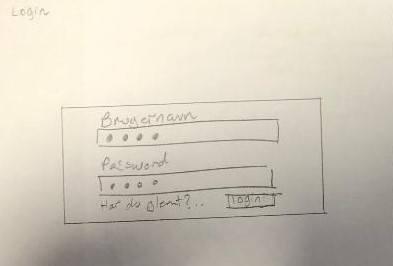
\includegraphics[width=\textwidth]{billeder/login-view.jpg}
			\caption{Login interface}
			\label{fig:1-Login}
		\end{subfigure}
		\quad
		\begin{subfigure}[b]{0.48\textwidth}
			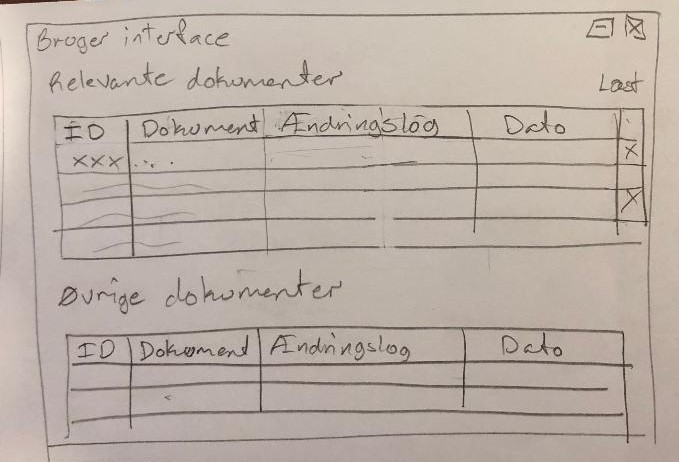
\includegraphics[width=\textwidth]{billeder/Main-view.jpg}
			\caption{Main page interface}
			\label{fig:1-Main}
		\end{subfigure}
\end{figure}
\begin{figure}[H]\ContinuedFloat
		\centering
		\begin{subfigure}[b]{0.48\textwidth}
			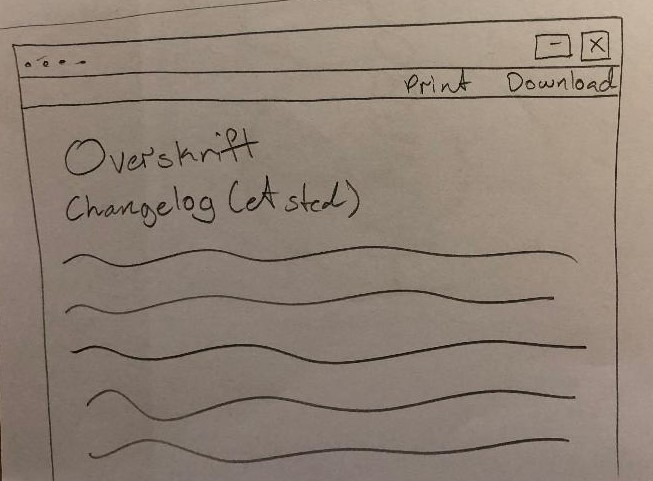
\includegraphics[width=\textwidth]{billeder/pdf-view.jpg}
			\caption{Pdf interface}
			\label{fig:1-pdf}
		\end{subfigure}
		\quad
		\begin{subfigure}[b]{0.48\textwidth}
			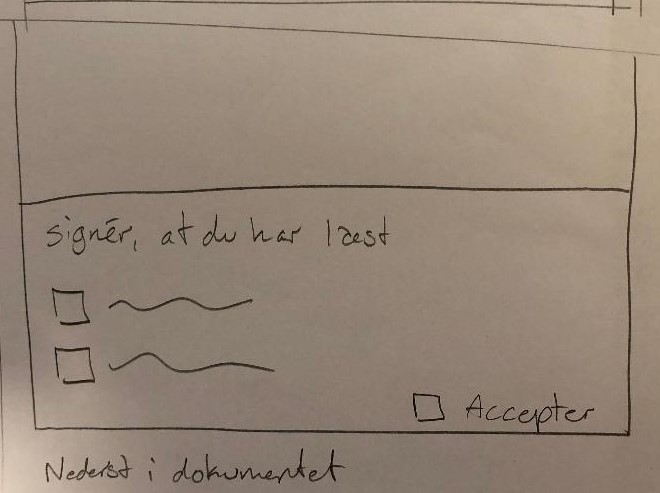
\includegraphics[width=\textwidth]{billeder/bottom-pdf-view.jpg}
			\caption{bottom of pdf view}
			\label{fig:1-bottom-pdf}
		\end{subfigure}
		\caption{Main interfaces and its connections}\label{fig:1-MainPages}
\end{figure}

%Second block of pictures
\begin{figure}[H]
	\centering
		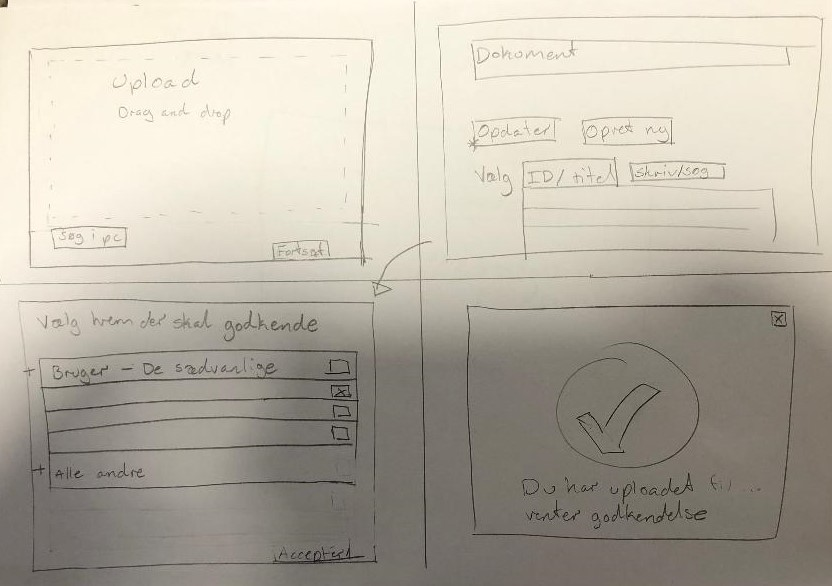
\includegraphics[width=0.65\textwidth]{billeder/Upload-view.jpg}
		\caption{The different interfaces during the upload process}
		\label{fig:1-Upload}
\end{figure}

%Third block of pictures
\begin{figure}[H]
	\centering
	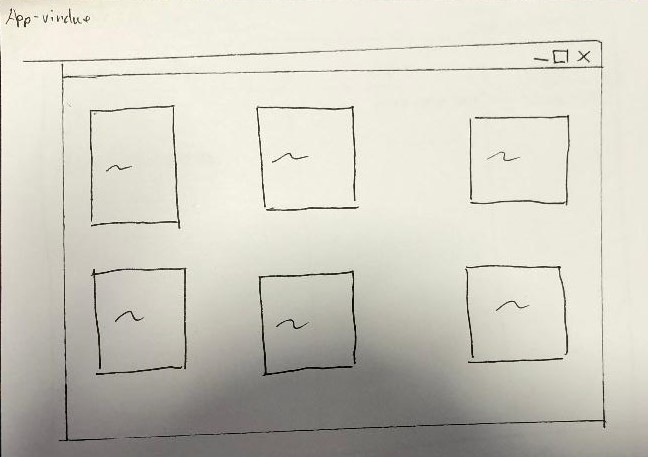
\includegraphics[width=0.5\textwidth]{billeder/app-view.jpg}
	\caption{Interface for first page after login}
	\label{fig:1-app-view}
\end{figure}

\section{Second sketches}\label{sec:Second-sketches}
\begin{figure}[H]
	\centering
	\begin{subfigure}[b]{0.48\textwidth}
		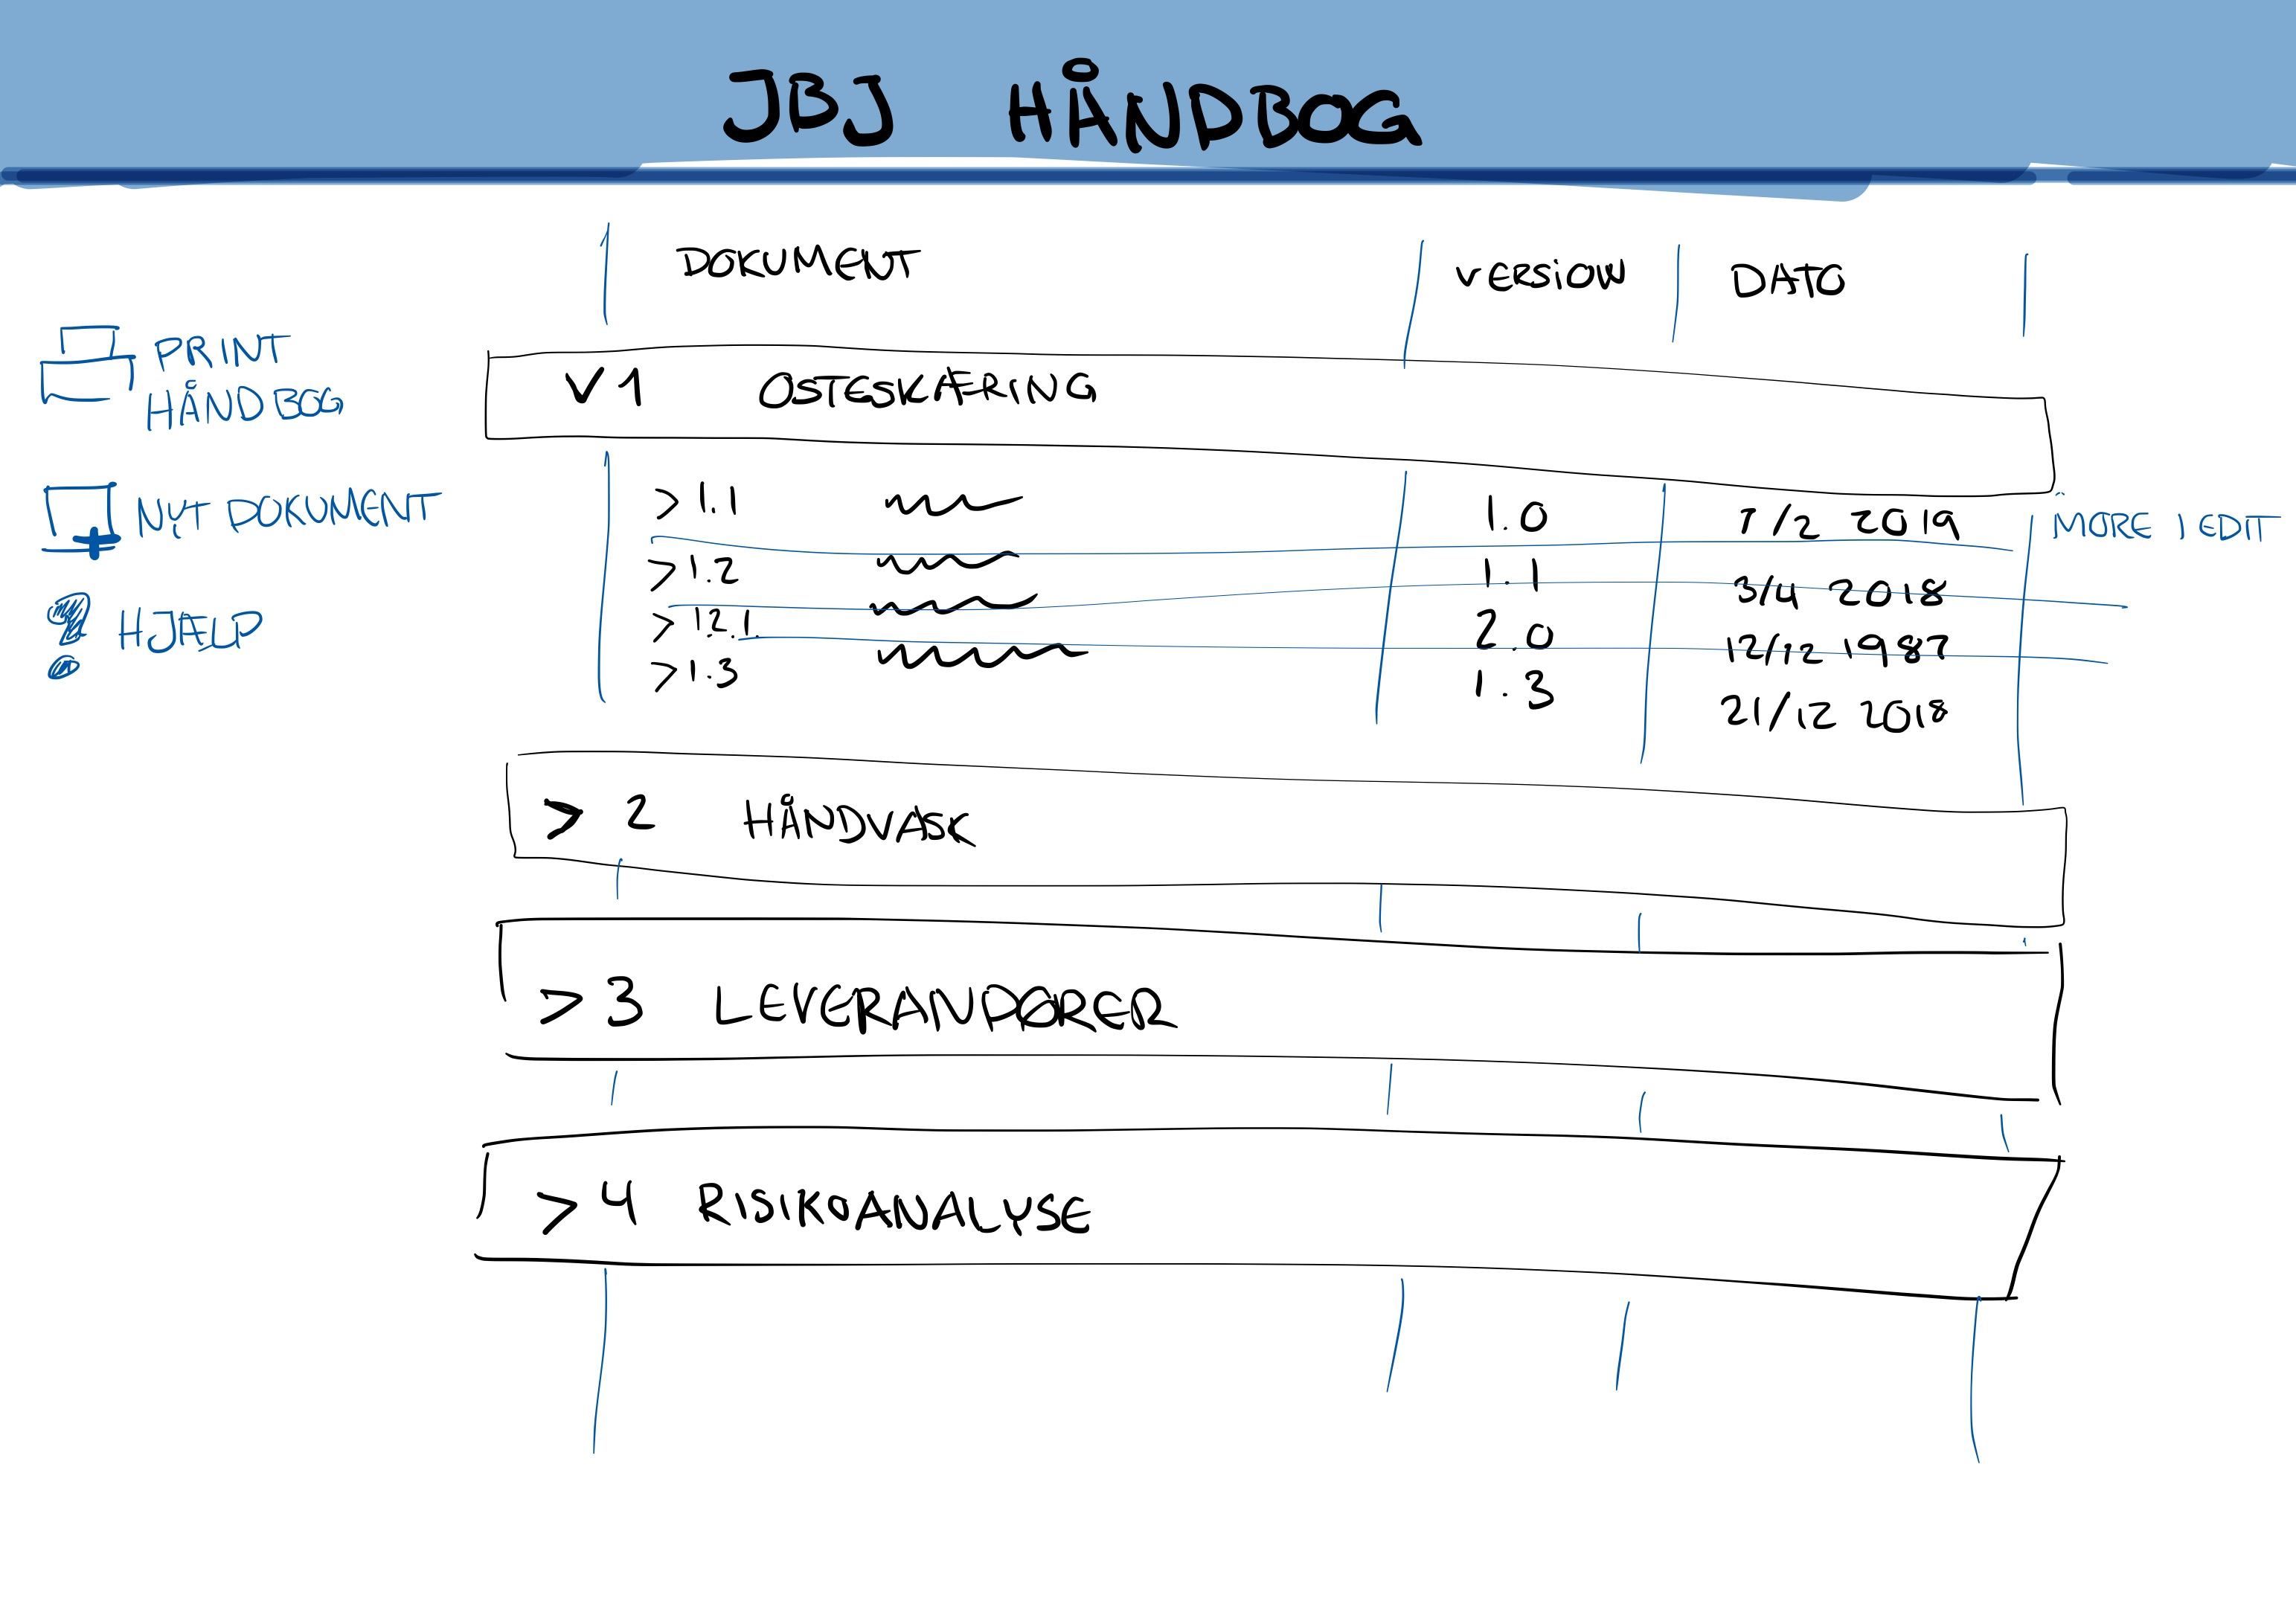
\includegraphics[width=\textwidth]{billeder/Main-view2.jpg}
		\caption{Main page interface}
		\label{fig:2-Main}
	\end{subfigure}
	\quad
	\begin{subfigure}[b]{0.48\textwidth}
		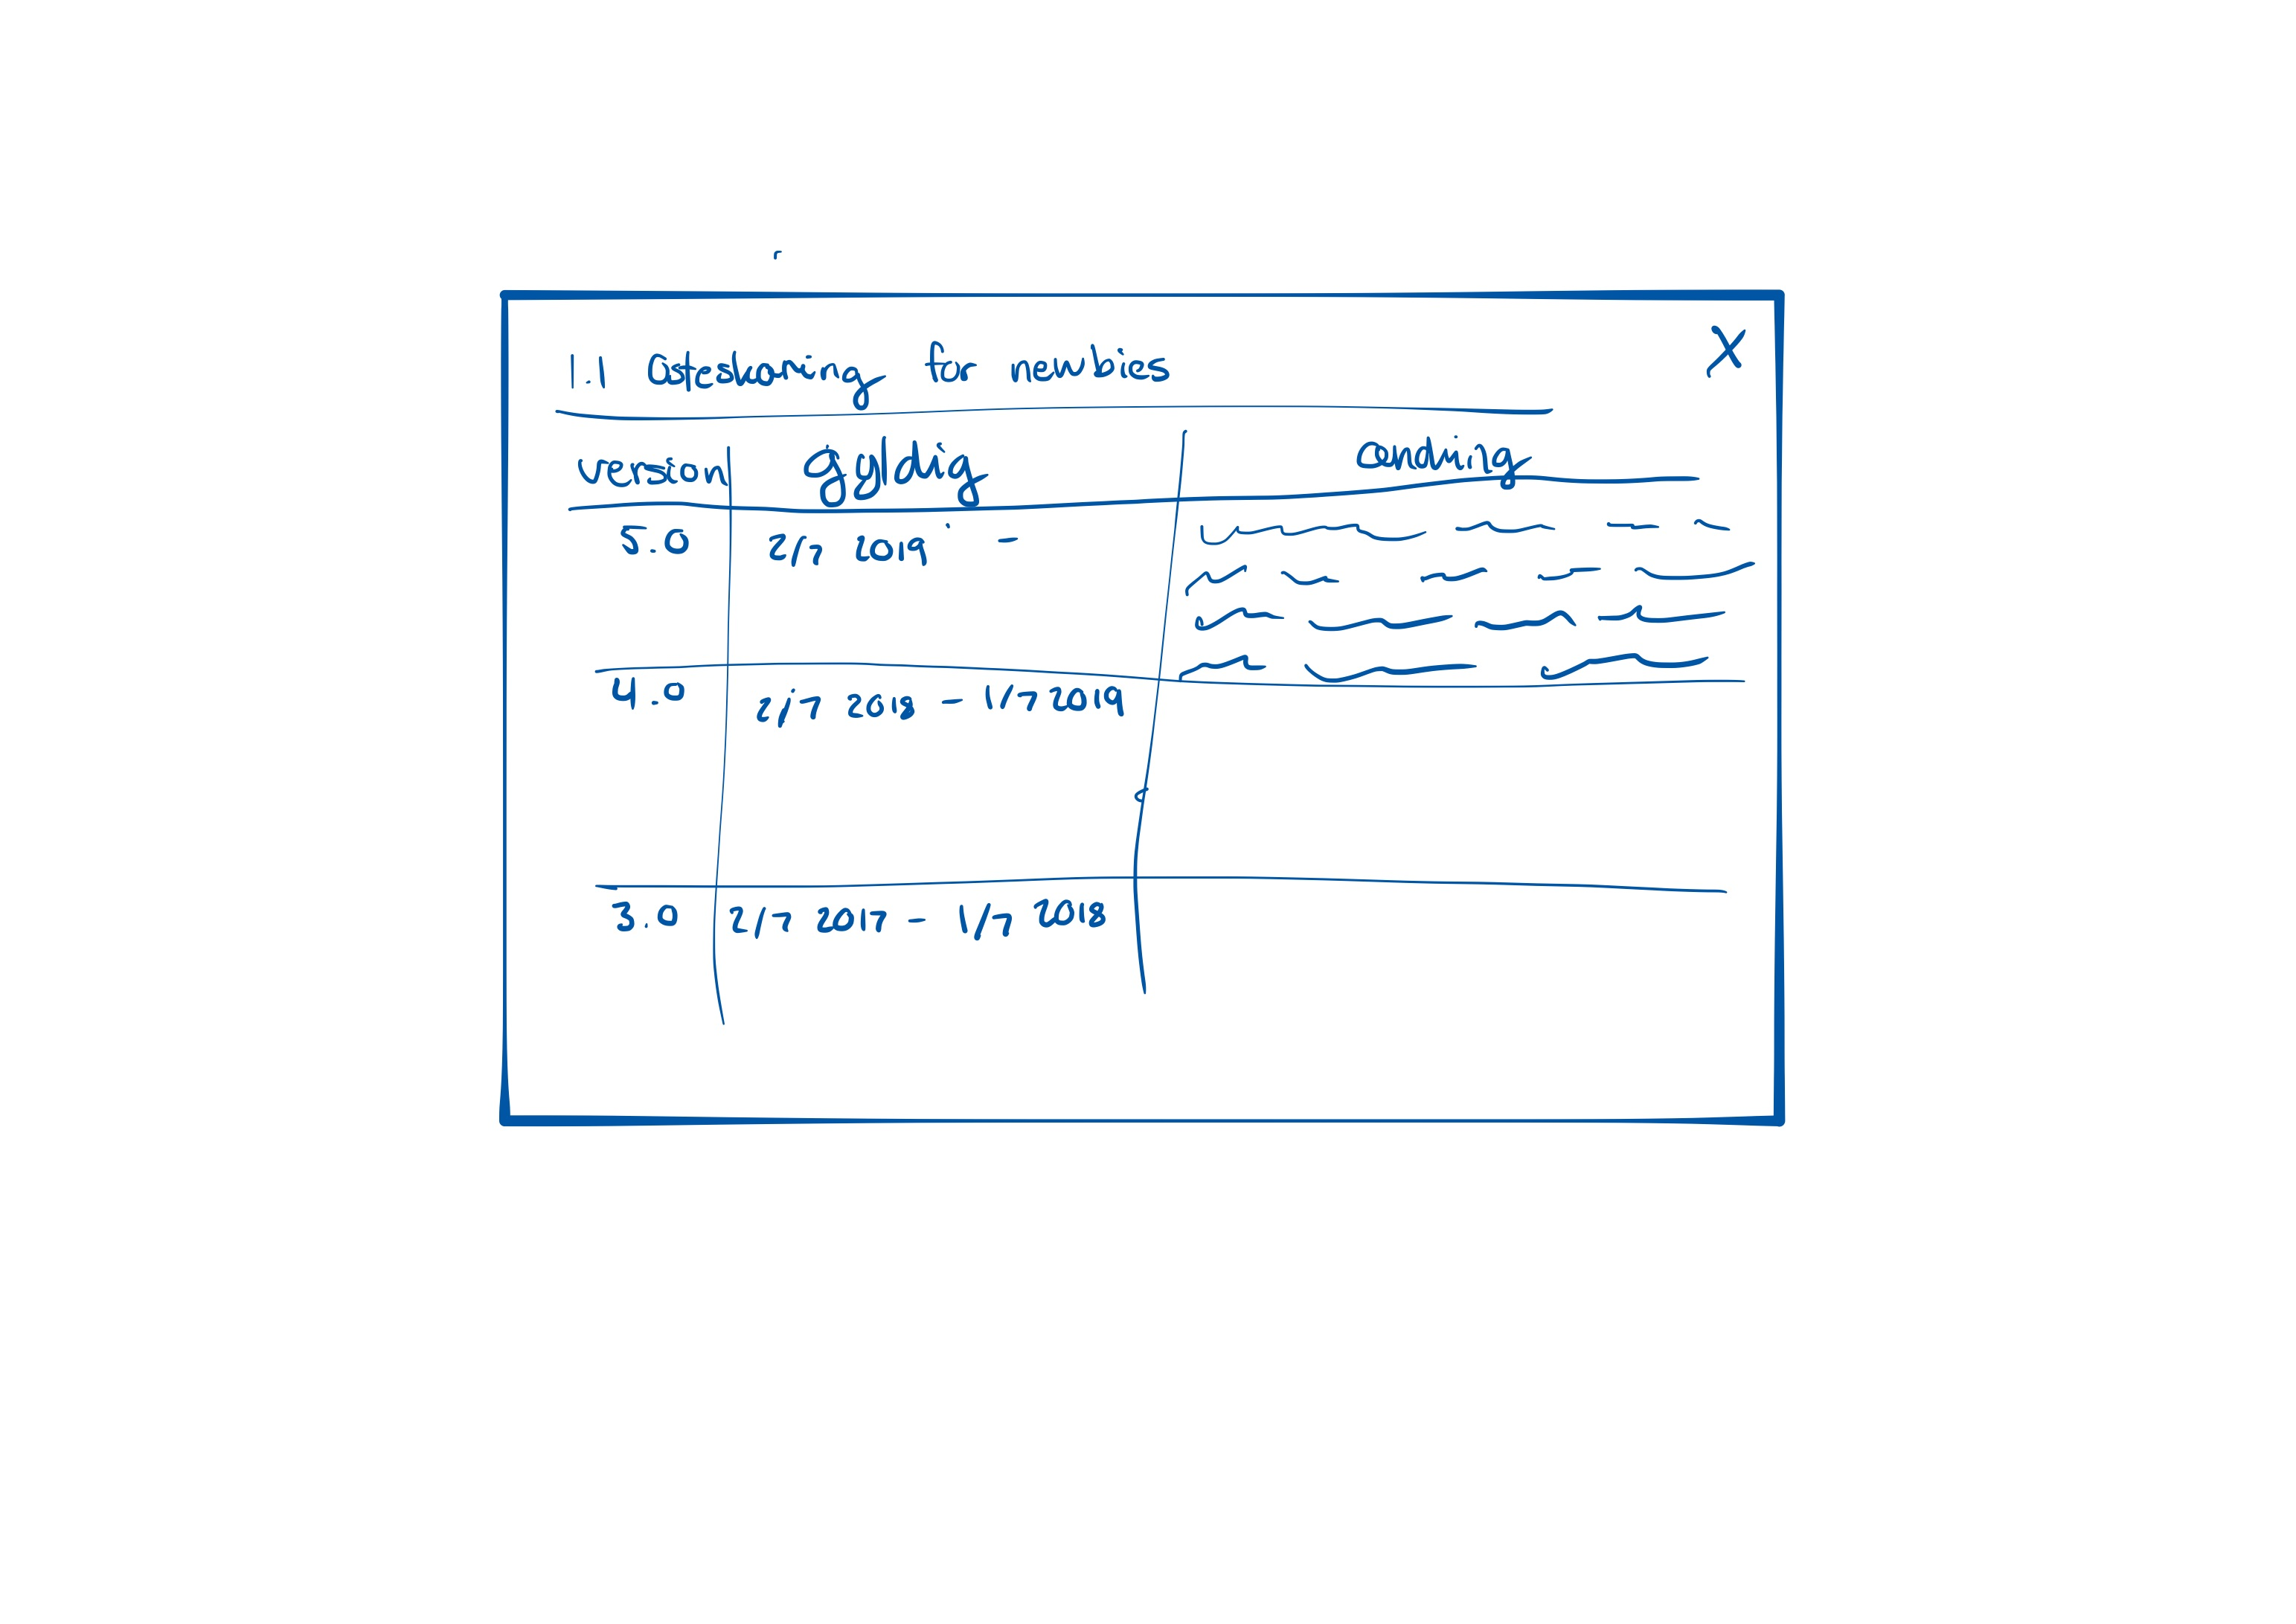
\includegraphics[width=\textwidth]{billeder/Archive-view2.jpg}
		\caption{Archive view of one document}
		\label{fig:2-Archive}
	\end{subfigure}
	\caption{Another idea of how to make the main interface and archive look as well as the archive for one document}
\end{figure}

\newpage
\section{Main interfaces from prototype for second meeting with Ipsen}\label{sec:1prototype}
%Første gruppering af billeder
\begin{figure}[H]
	\centering
	\begin{subfigure}[b]{0.48\textwidth}
		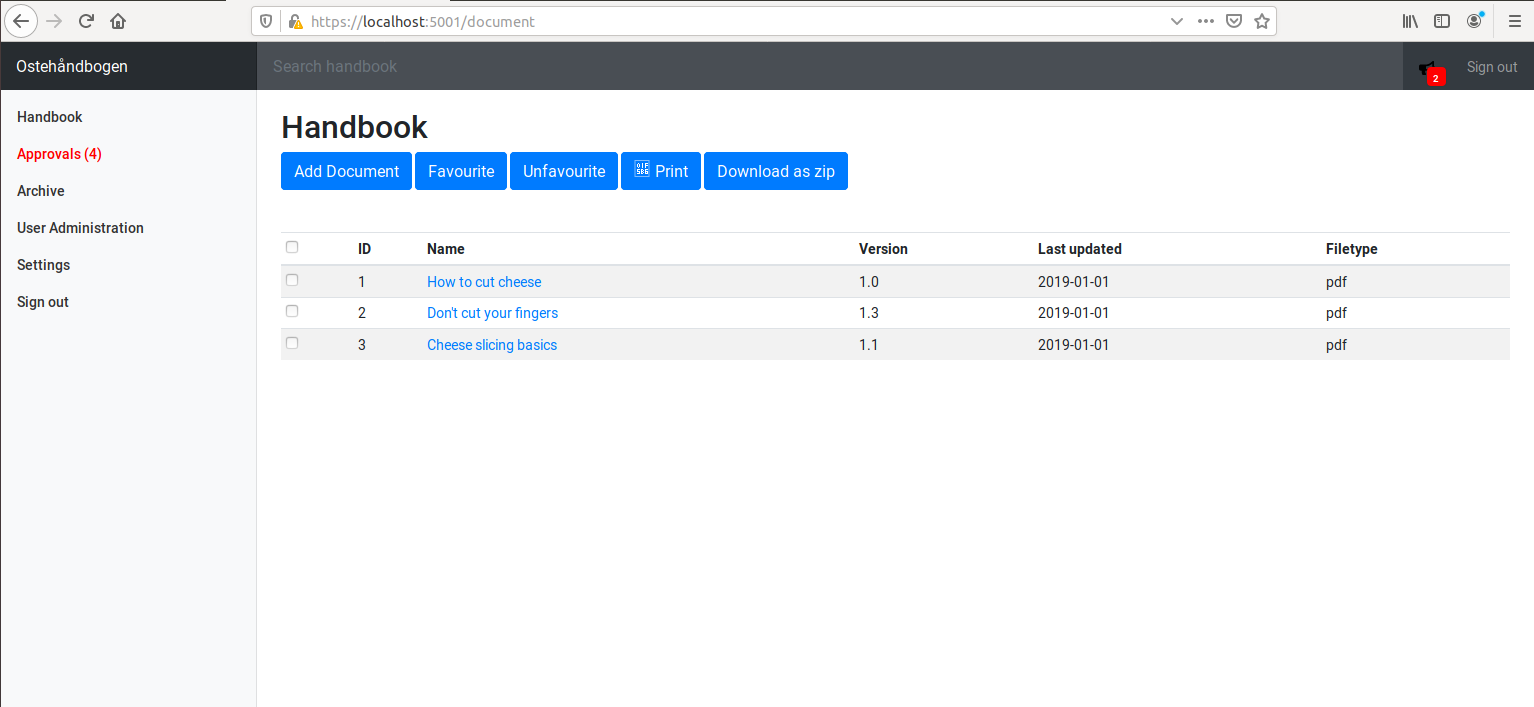
\includegraphics[width=\textwidth]{billeder/iteration1Prototyper/Handbook.png}
		\caption{Main interface}
		\label{fig:3-main}
	\end{subfigure}
	\quad
	\begin{subfigure}[b]{0.48\textwidth}
		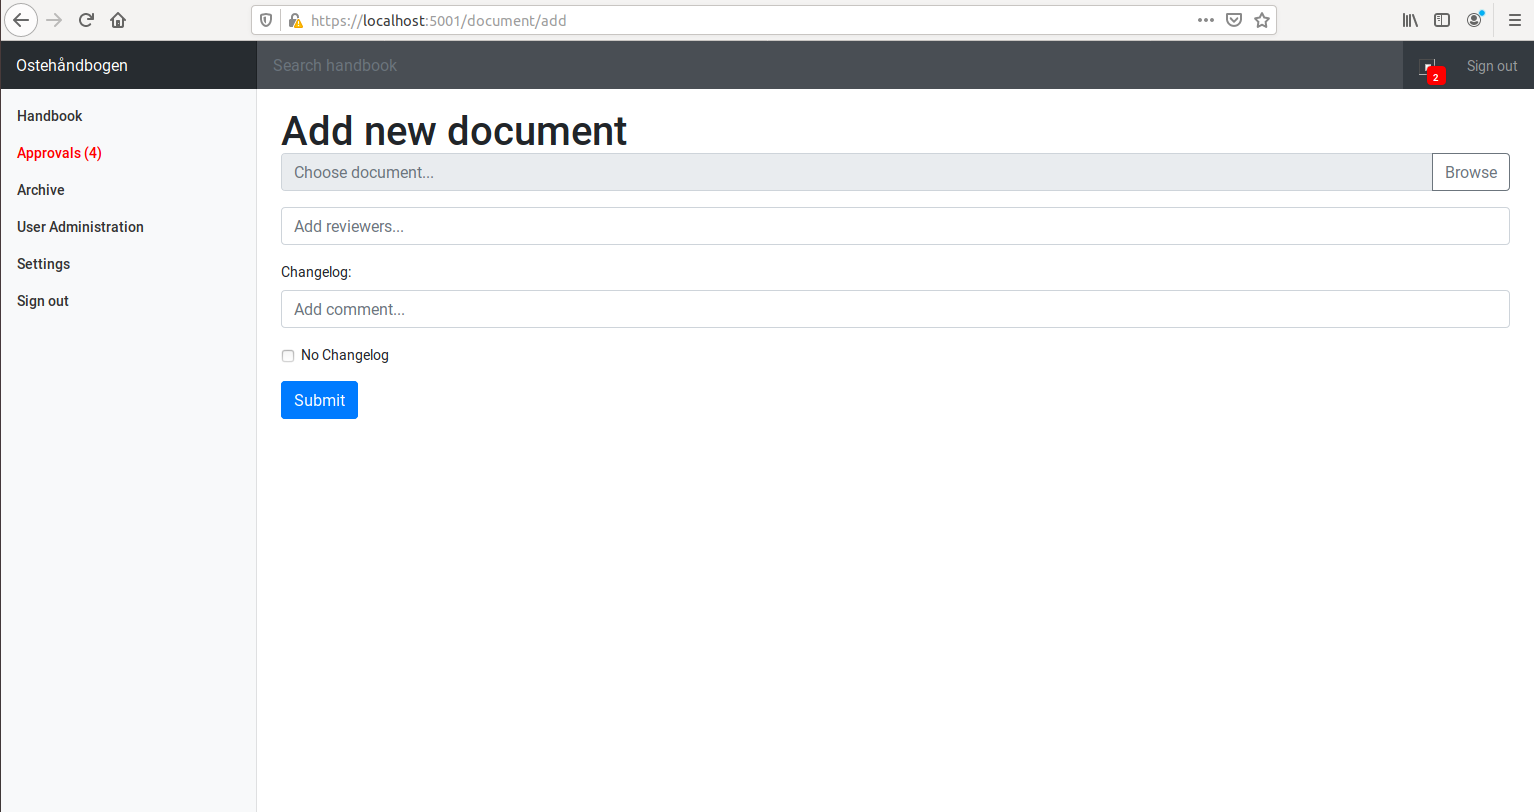
\includegraphics[width=\textwidth]{billeder/iteration1Prototyper/Add-Document.png}
		\caption{View after pressing ''Add Document'' in main interface}
		\label{fig:3-addDoc}
	\end{subfigure}
\end{figure}
\begin{figure}[H]\ContinuedFloat
	\centering
	\begin{subfigure}[b]{0.48\textwidth}
		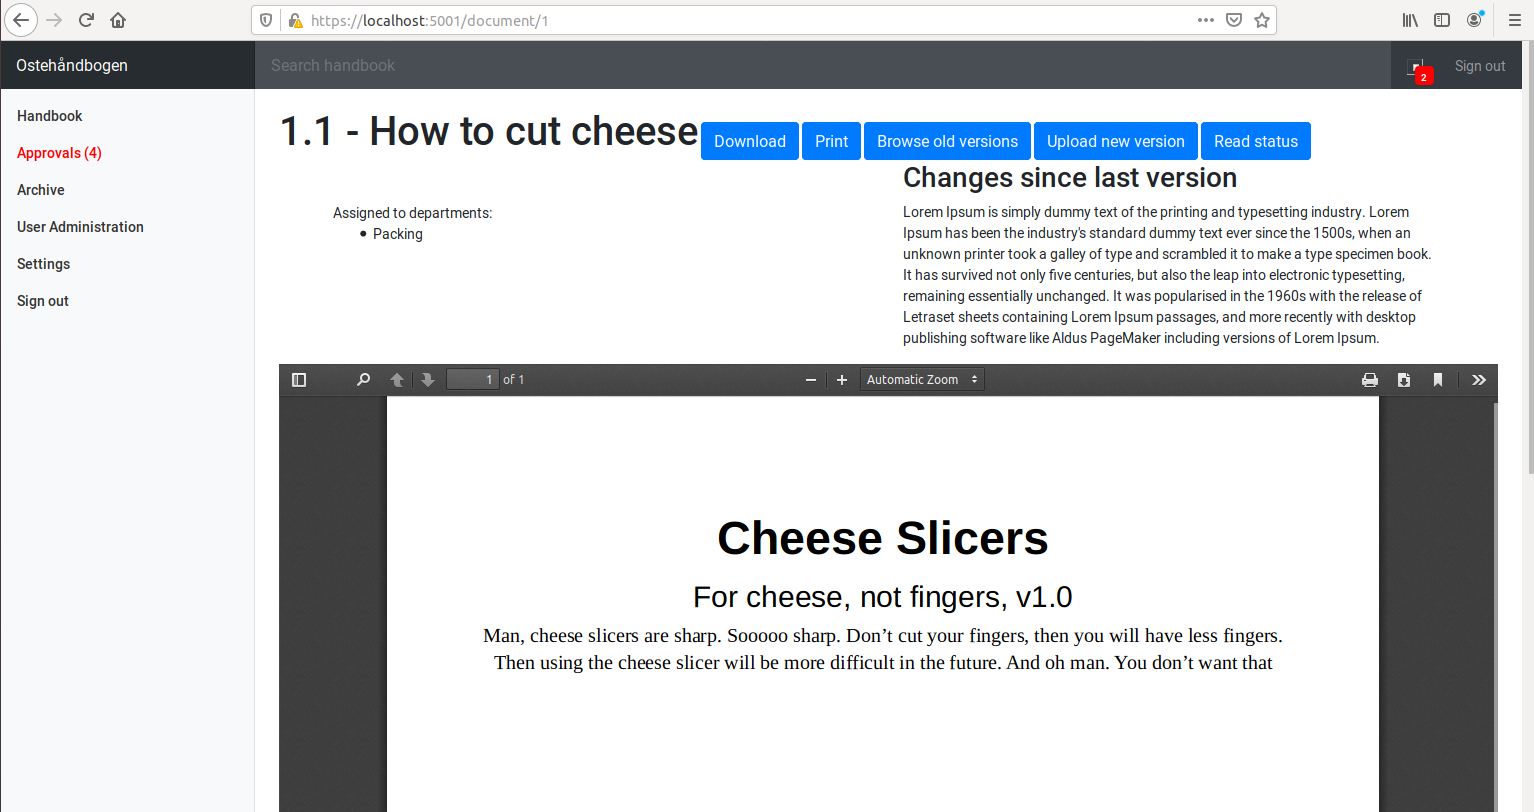
\includegraphics[width=\textwidth]{billeder/iteration1Prototyper/Document-view.png}
		\caption{View of active version in specific Document}
		\label{fig:3-DocView}
	\end{subfigure}
	\quad
	\begin{subfigure}[b]{0.48\textwidth}
		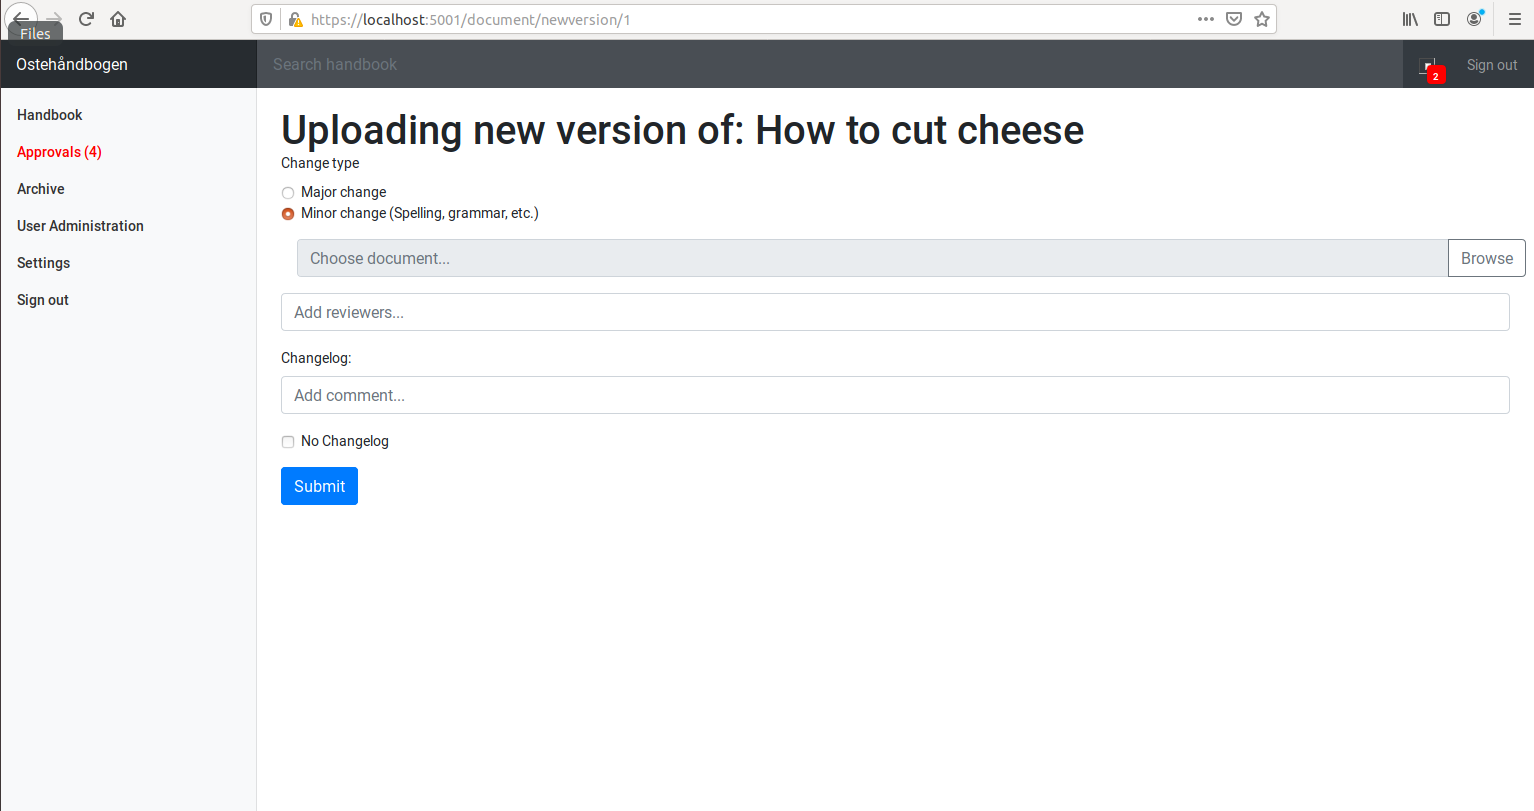
\includegraphics[width=\textwidth]{billeder/iteration1Prototyper/Upload-version.png}
		\caption{View after pressing ''Upload new version''}
		\label{fig:3-UploadVer}
	\end{subfigure}
	\caption{Interfaces connected to main page}\label{fig:3-MainPages}
\end{figure}

%Anden gruppering af billeder
\begin{figure}[H]
	\centering
	\begin{subfigure}[b]{0.48\textwidth}
		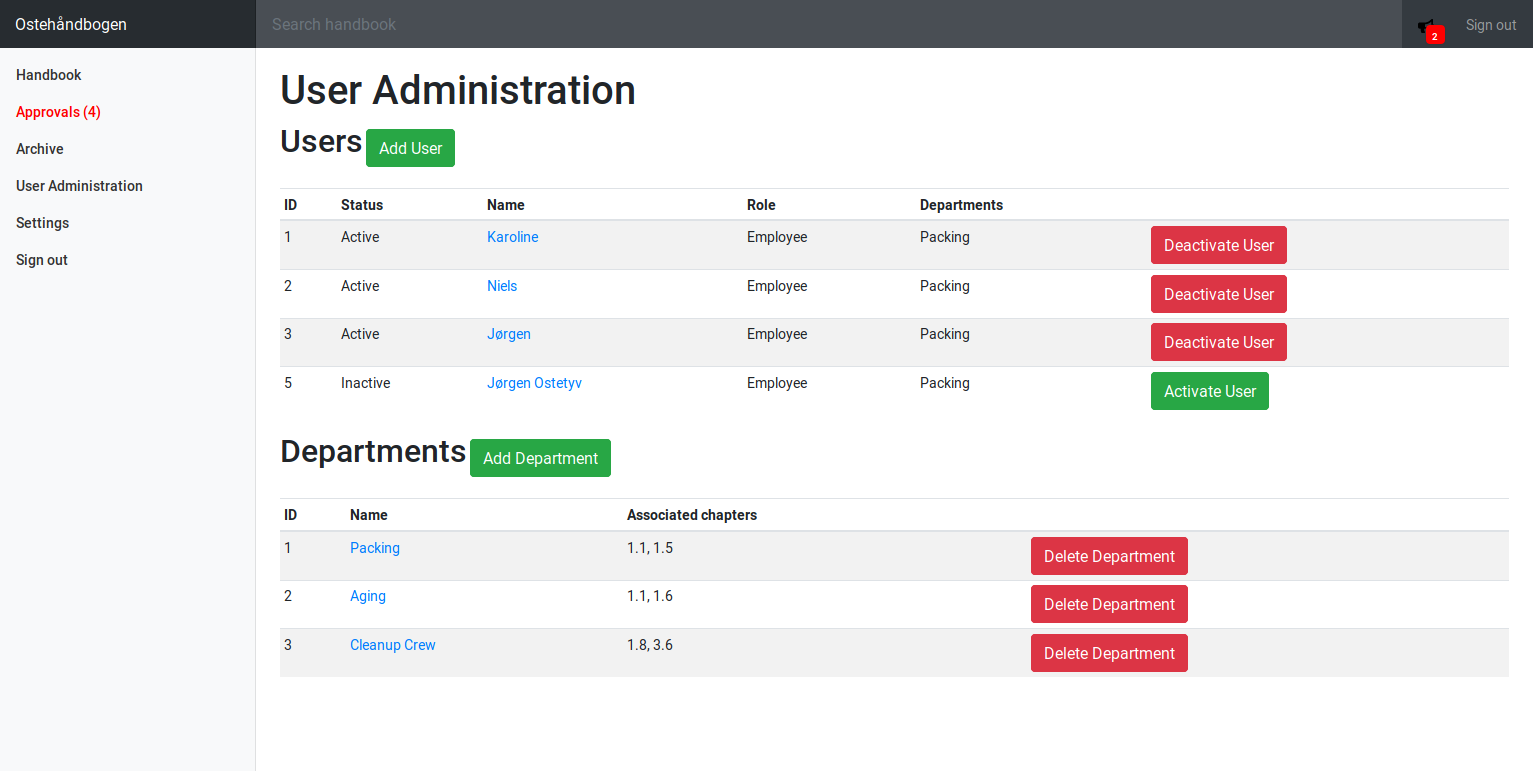
\includegraphics[width=\textwidth]{billeder/iteration1Prototyper/UserAdministration.png}
		\caption{User administration interface}
		\label{fig:3-UserAdmin}
	\end{subfigure}
	\quad
	\begin{subfigure}[b]{0.48\textwidth}
		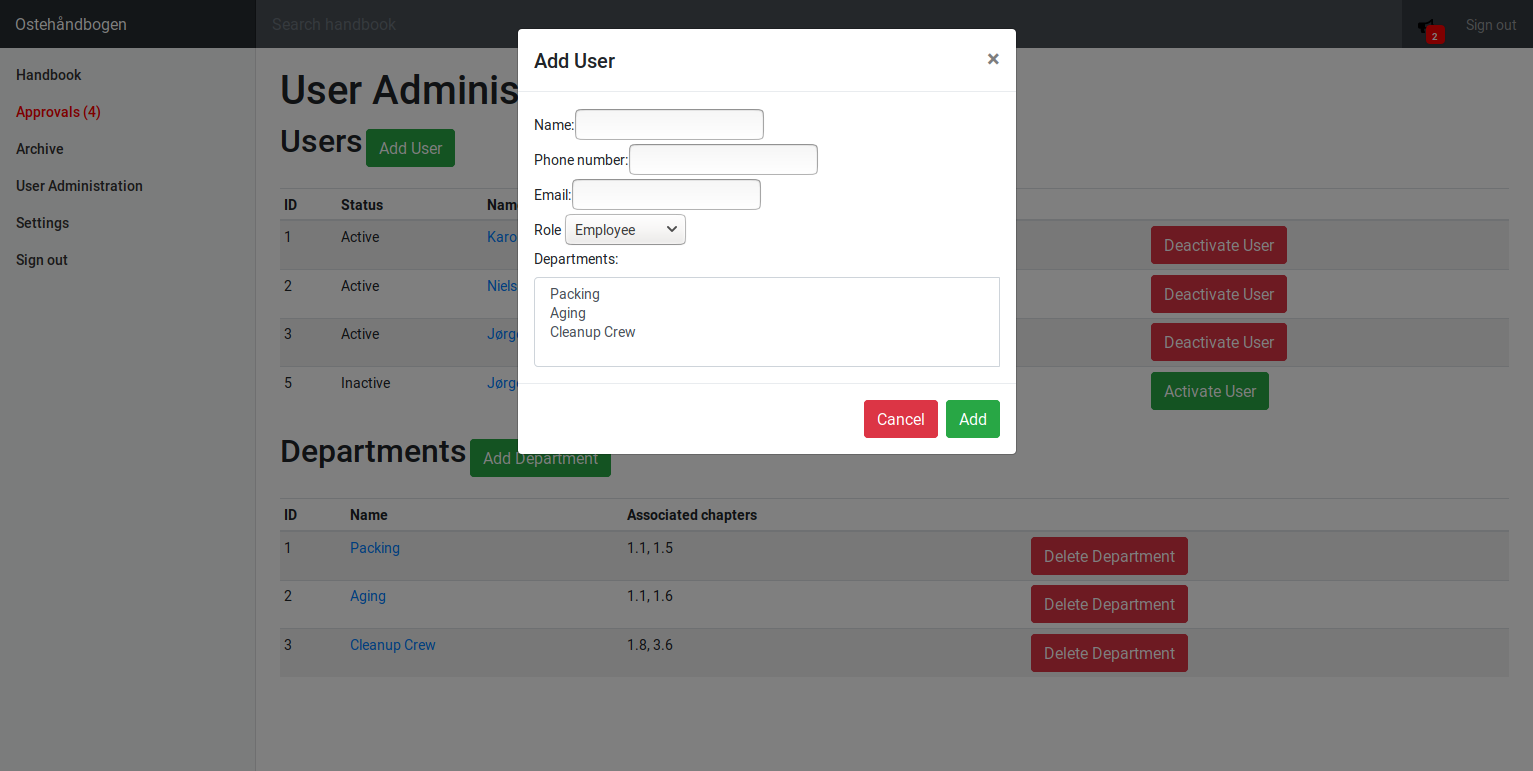
\includegraphics[width=\textwidth]{billeder/iteration1Prototyper/AddUser.png}
		\caption{Add new user view}
		\label{fig:3-addUser}
	\end{subfigure}
\end{figure}
\begin{figure}[H]\ContinuedFloat
	\centering
	\begin{subfigure}[b]{0.48\textwidth}
		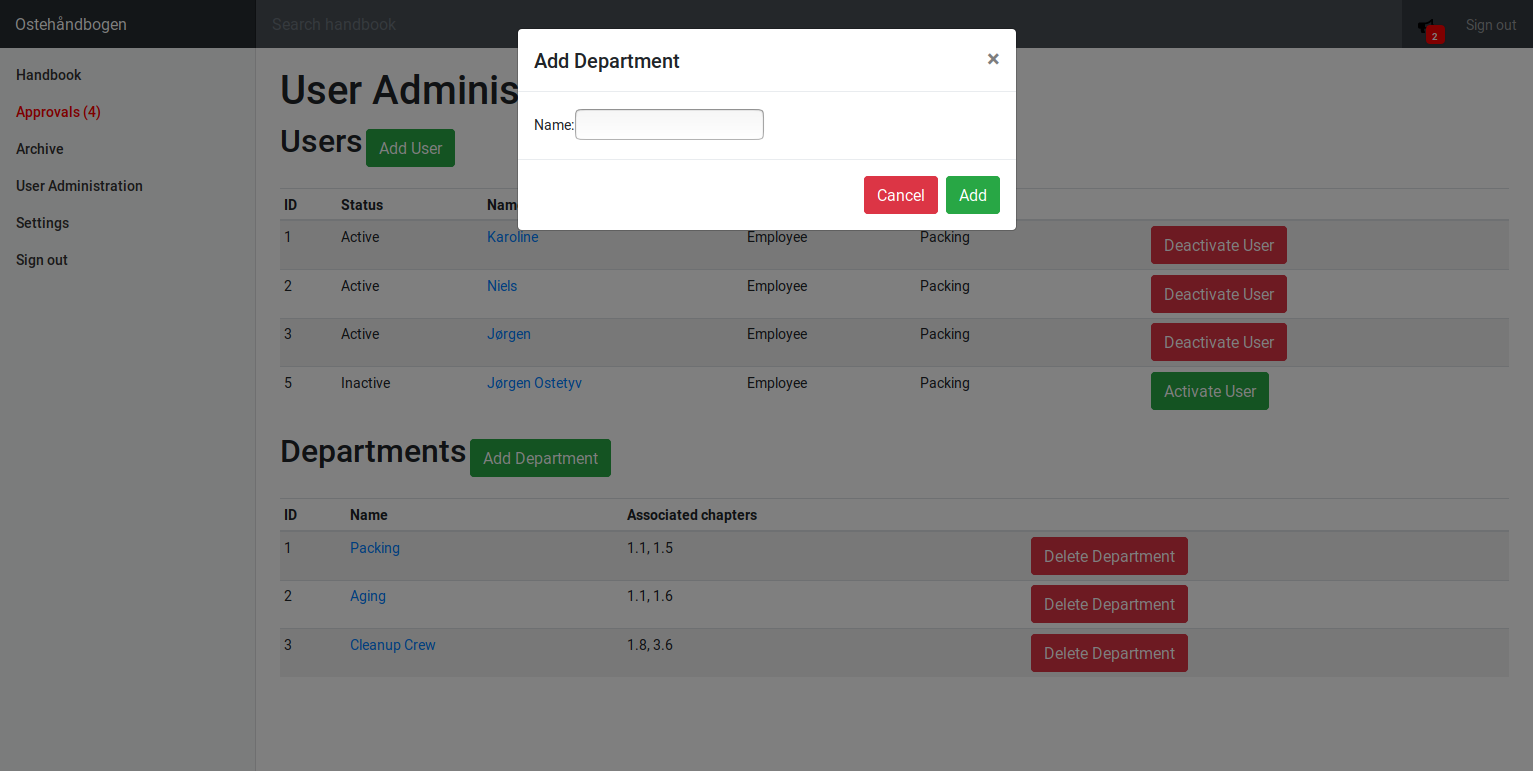
\includegraphics[width=\textwidth]{billeder/iteration1Prototyper/AddDepartment.png}
		\caption{Add new department}
		\label{fig:3-AddDep}
	\end{subfigure}
	\quad
	\begin{subfigure}[b]{0.48\textwidth}
		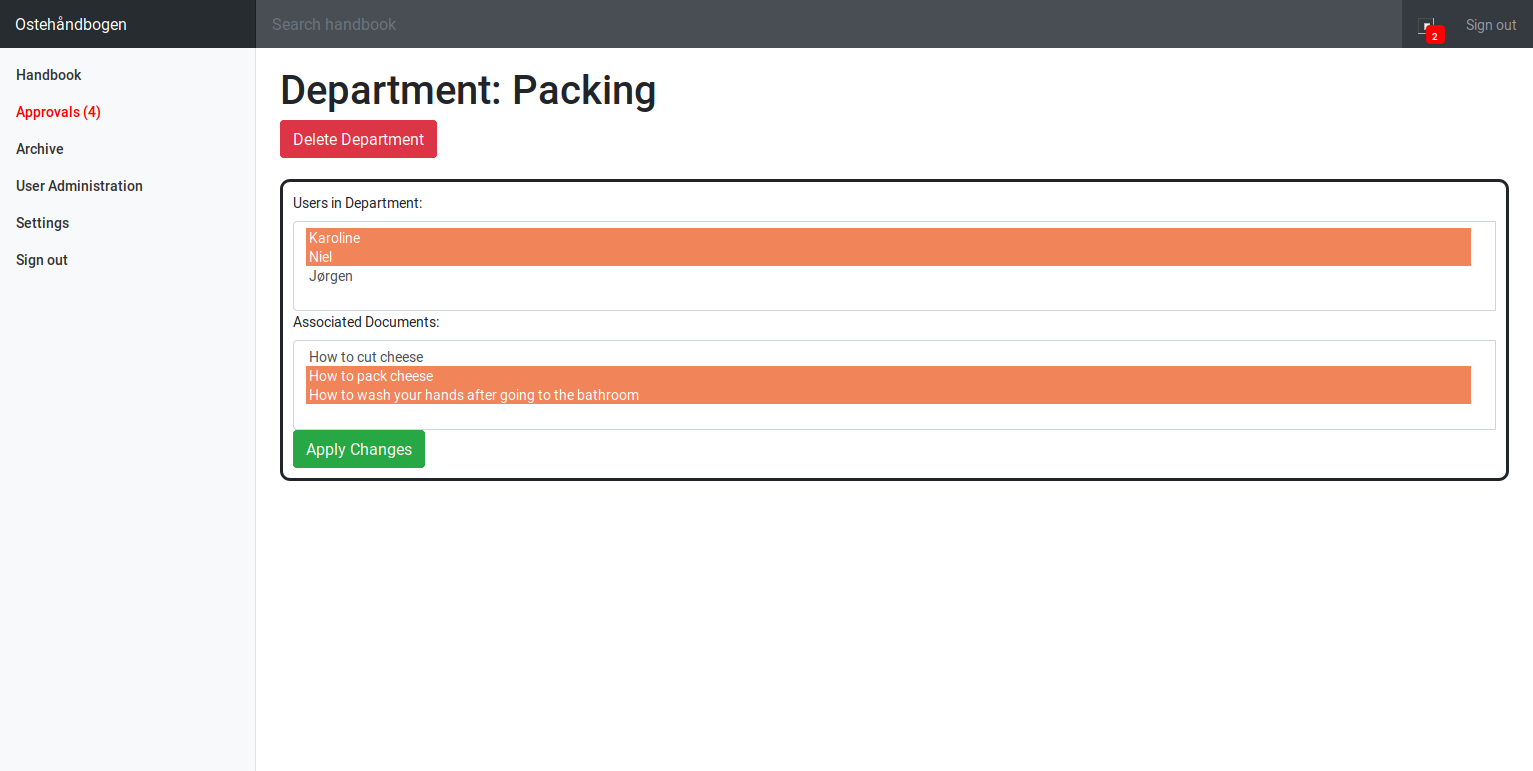
\includegraphics[width=\textwidth]{billeder/iteration1Prototyper/DepartmentEdit.png}
		\caption{Edit existing department}
		\label{fig:3-EditDep}
	\end{subfigure}
	\caption{Interfaces connected user administration}\label{fig:3-UserAdminPages}
\end{figure}

%Tredje gruppering af billeder
\begin{figure}[H]
	\centering
	\begin{subfigure}[b]{0.48\textwidth}
		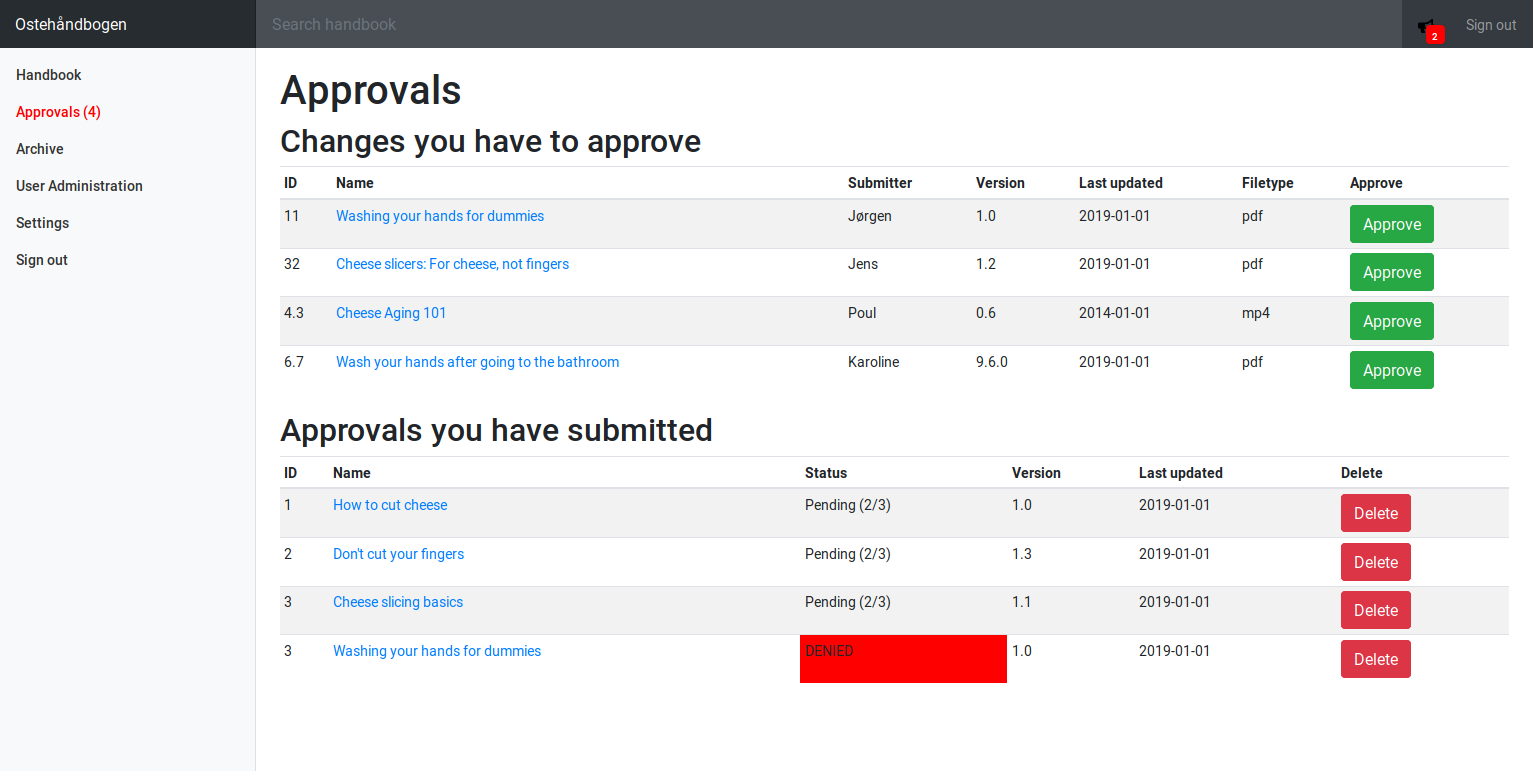
\includegraphics[width=\textwidth]{billeder/iteration1Prototyper/Approval.png}
		\caption{Approval interface}
		\label{fig:3-approve}
	\end{subfigure}
	\quad
	\begin{subfigure}[b]{0.48\textwidth}
		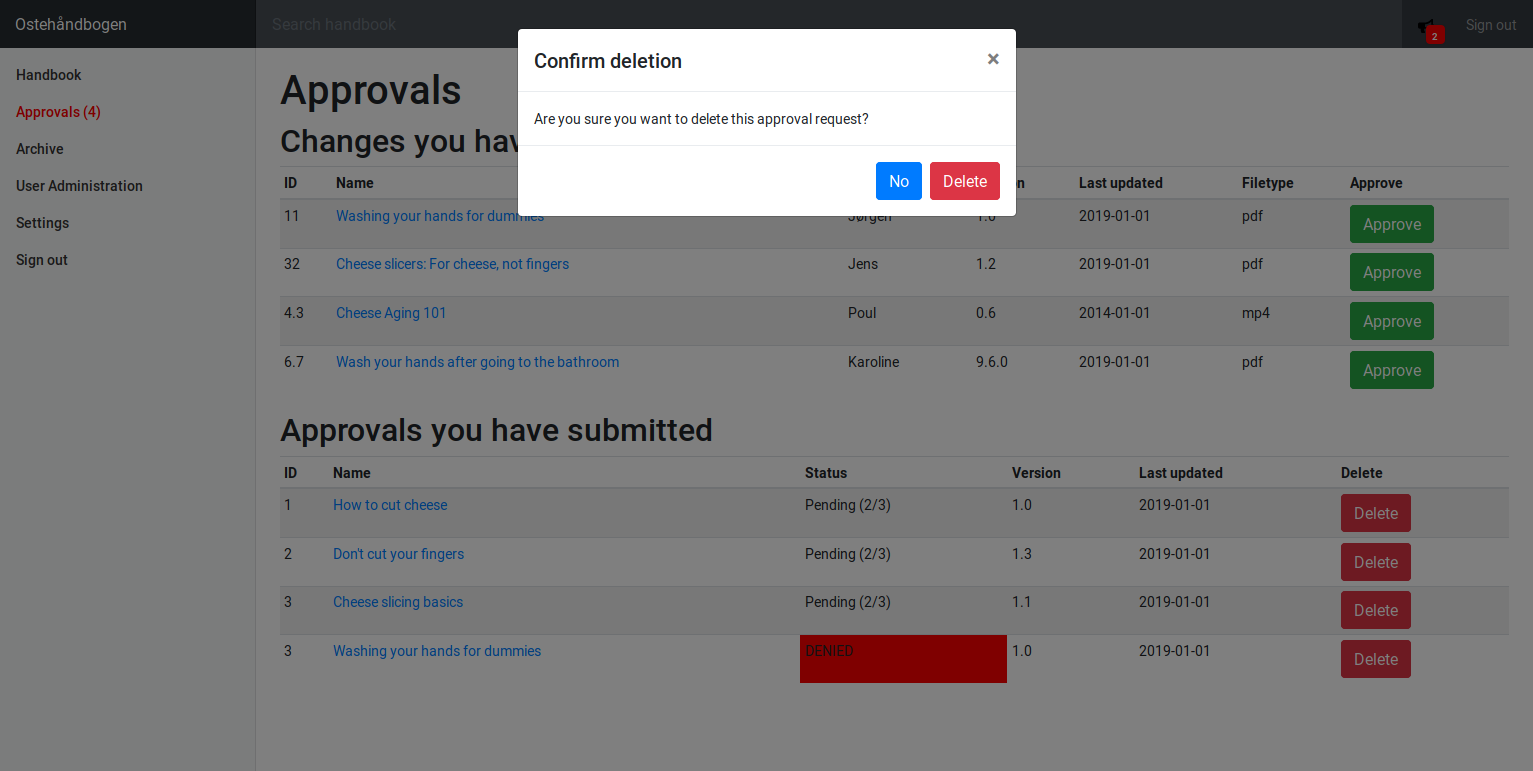
\includegraphics[width=\textwidth]{billeder/iteration1Prototyper/ApprovalDenial.png}
		\caption{Pop up when denying approval.}
		\label{fig:3-ApproveDenial}
	\end{subfigure}
\end{figure}
\begin{figure}[H]\ContinuedFloat
	\centering
	\begin{subfigure}[b]{0.48\textwidth}
		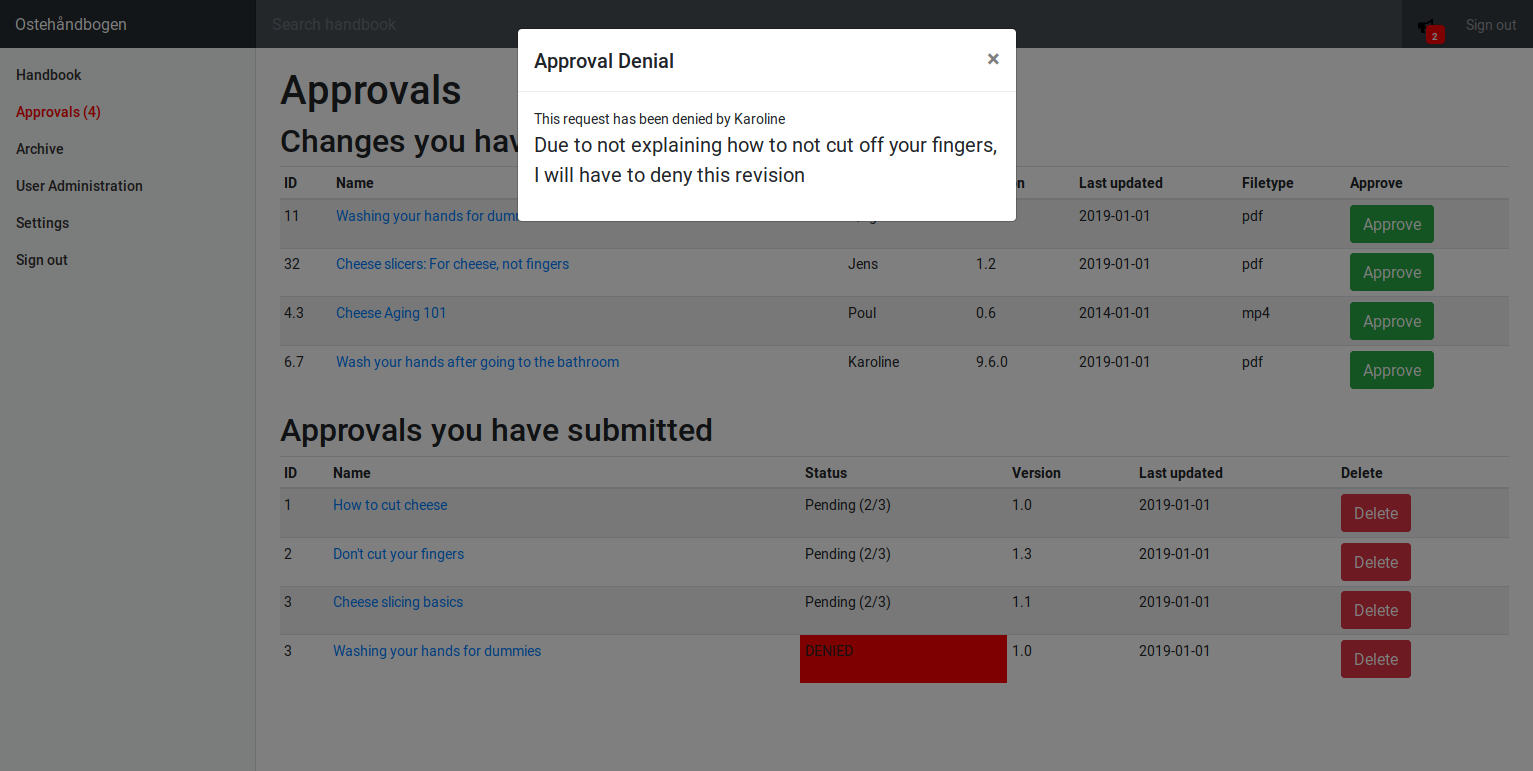
\includegraphics[width=\textwidth]{billeder/iteration1Prototyper/ApprovalDenied.png}
		\caption{when someone else has denied the approval}
		\label{fig:3-ApproveDenied}
	\end{subfigure}
	\quad
	\begin{subfigure}[b]{0.48\textwidth}
		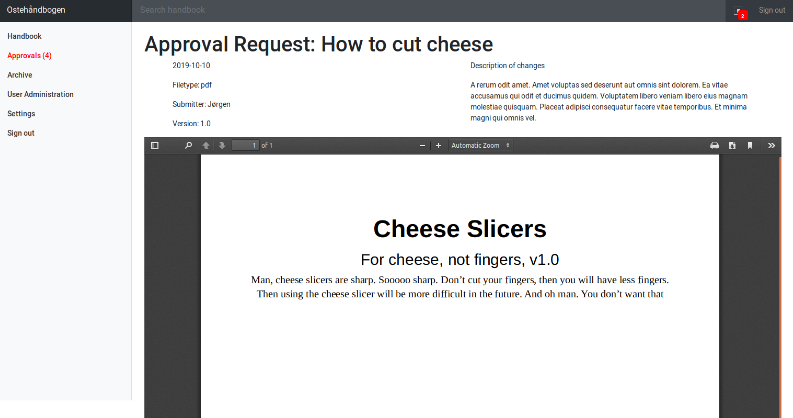
\includegraphics[width=\textwidth]{billeder/iteration1Prototyper/ApprovalRequest.png}
		\caption{Detailed view of an approval request.}
		\label{fig:3-ApproveRequest}
	\end{subfigure}
	\caption{Interfaces connected to Approval process}\label{fig:3-AprovalPages}
\end{figure}

%Fjerde gruppering af billeder
\begin{figure}[H]
	\centering
	\begin{subfigure}[b]{0.48\textwidth}
		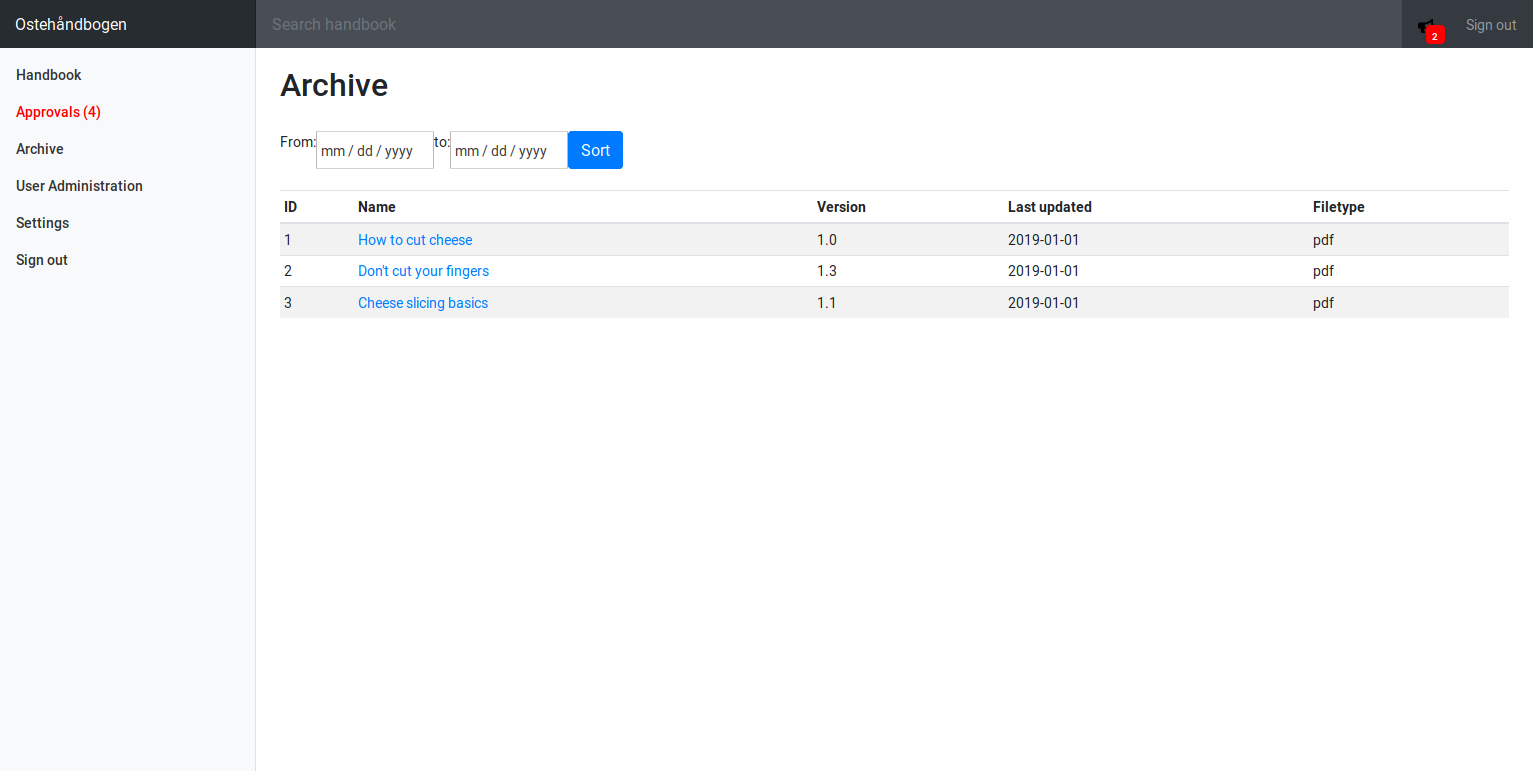
\includegraphics[width=\textwidth]{billeder/iteration1Prototyper/Archive.png}
		\caption{Archive interface}
		\label{fig:3-archive}
	\end{subfigure}
	\quad
	\begin{subfigure}[b]{0.48\textwidth}
		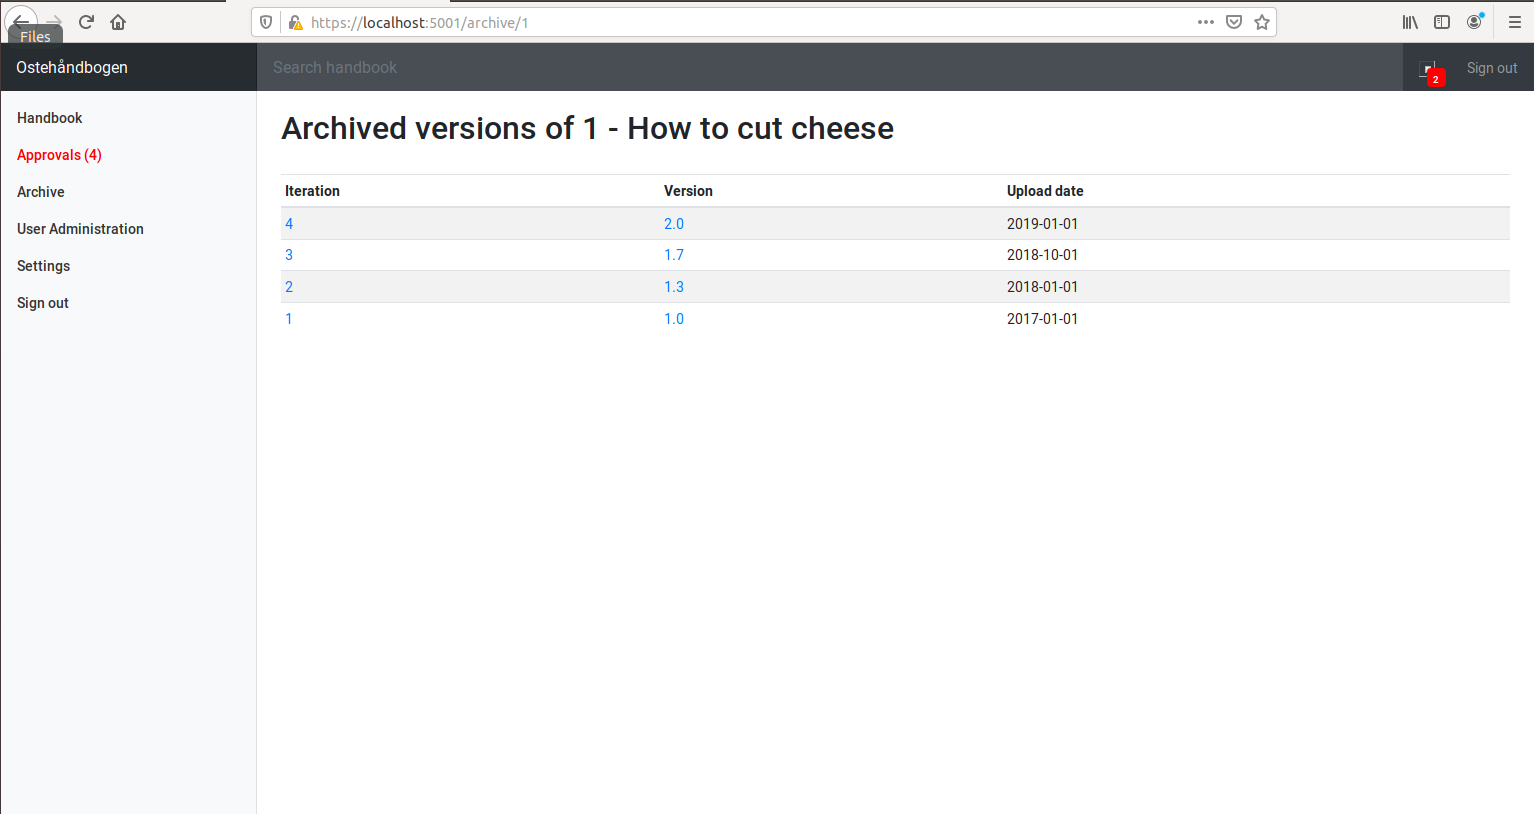
\includegraphics[width=\textwidth]{billeder/iteration1Prototyper/Archive-Version1.png}
		\caption{Archive of a specific document}
		\label{fig:3-ArchiveVersion}
	\end{subfigure}
	\caption{Interfaces connected to the archive}\label{fig:3-ArchivePages}
\end{figure}

\chapter{Second iteration prototypes}\label{chap:2-Prototypes}
\section{Mock-up}\label{sec:Mock}

\begin{figure}[H]
	\centering
	\begin{subfigure}[b]{0.48\textwidth}
		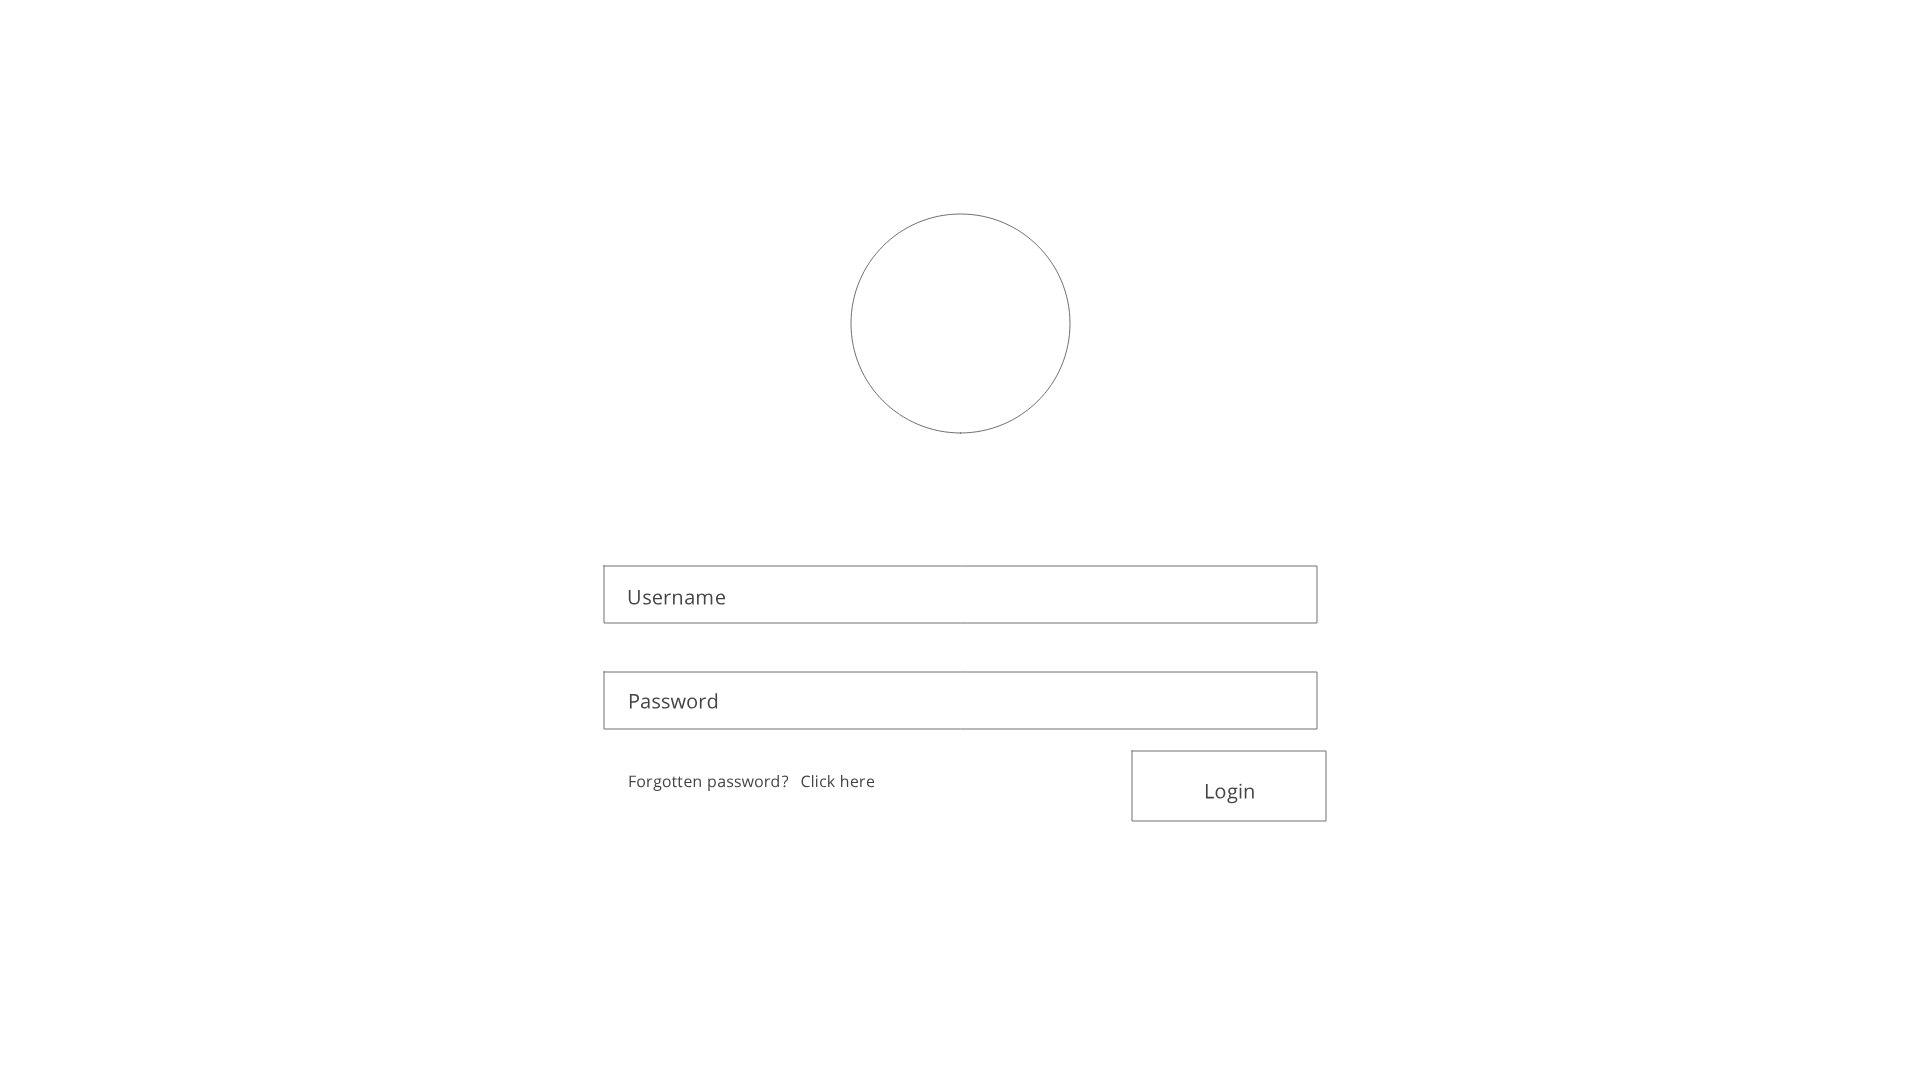
\includegraphics[width=\textwidth]{billeder/iteration2Prototyper/Page_1.jpg}
		\caption{Login interface}
		\label{fig:4-Login}
	\end{subfigure}
	\quad
	\begin{subfigure}[b]{0.48\textwidth}
		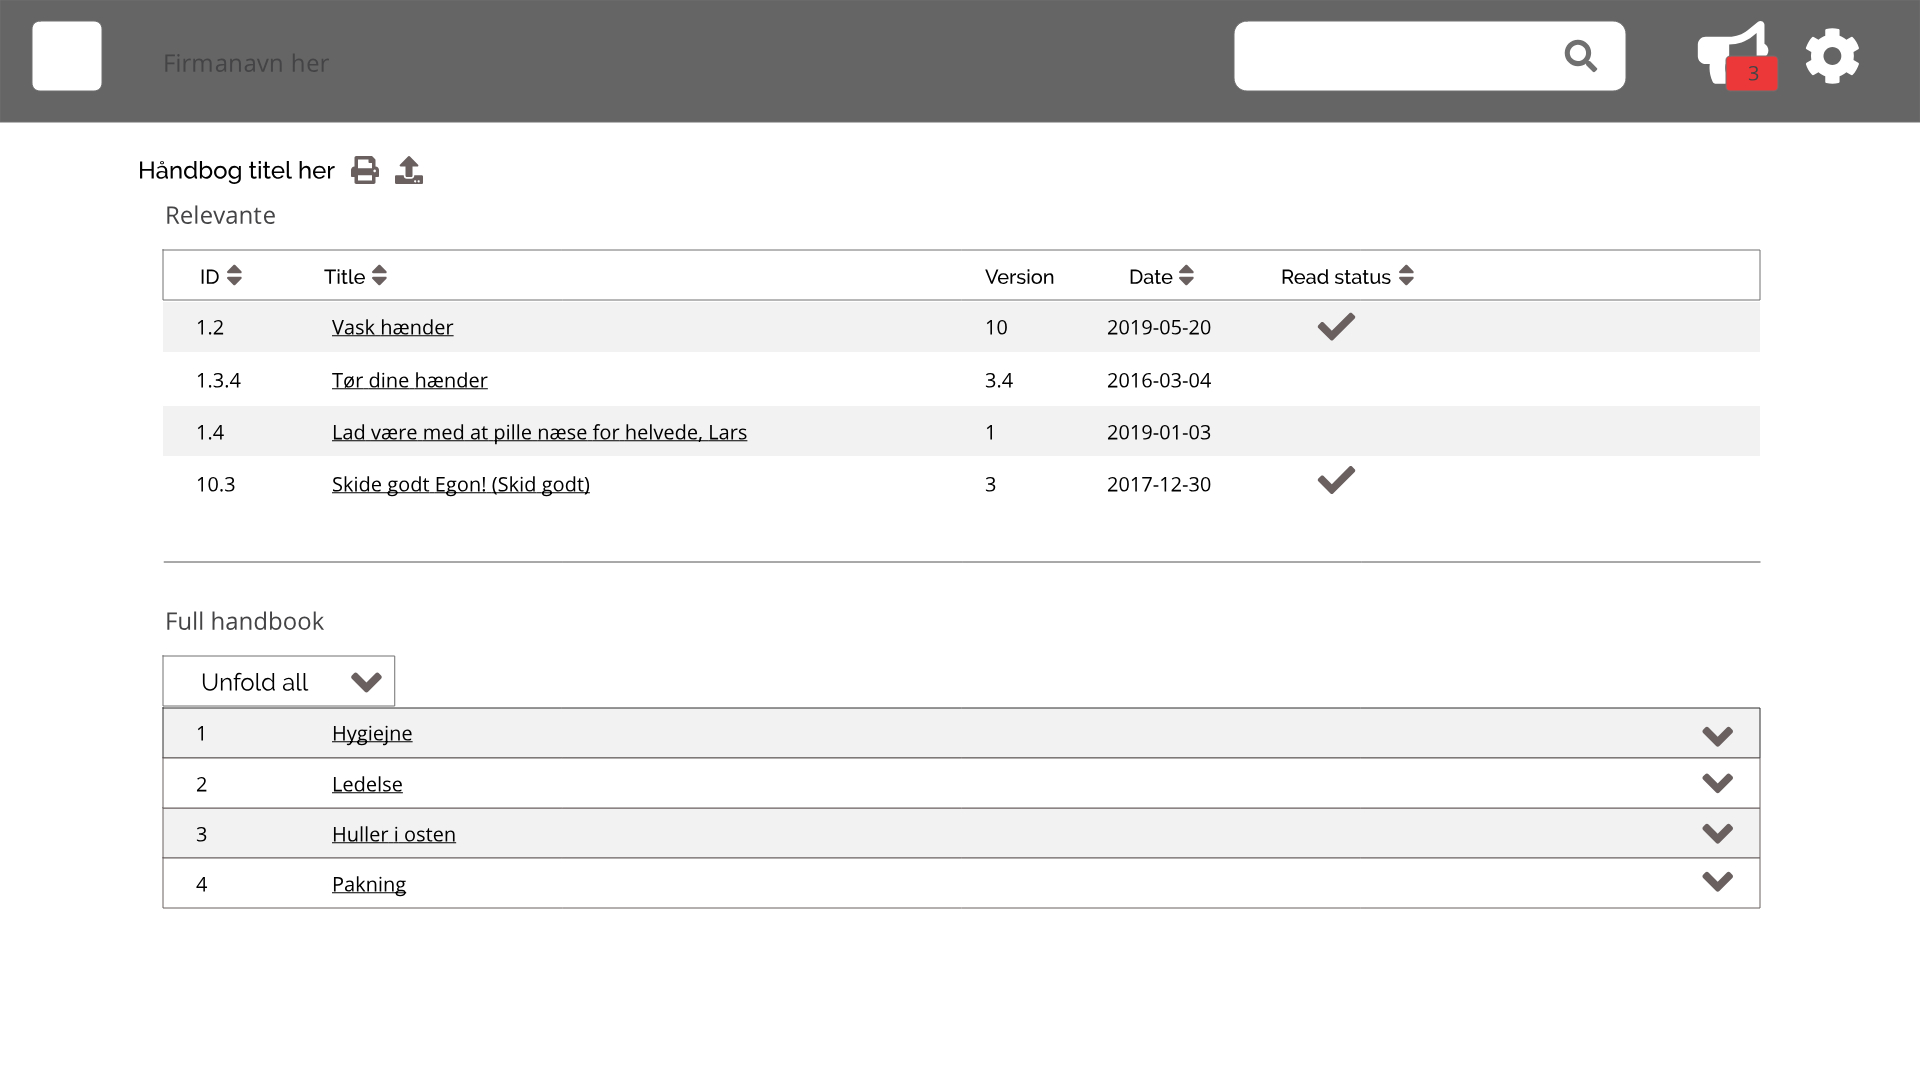
\includegraphics[width=\textwidth]{billeder/iteration2Prototyper/Page_2.jpg}
		\caption{Main page interface for writer}
		\label{fig:4-Main}
	\end{subfigure}
\end{figure}
\begin{figure}[H]\ContinuedFloat
	\centering
	\begin{subfigure}[b]{0.48\textwidth}
		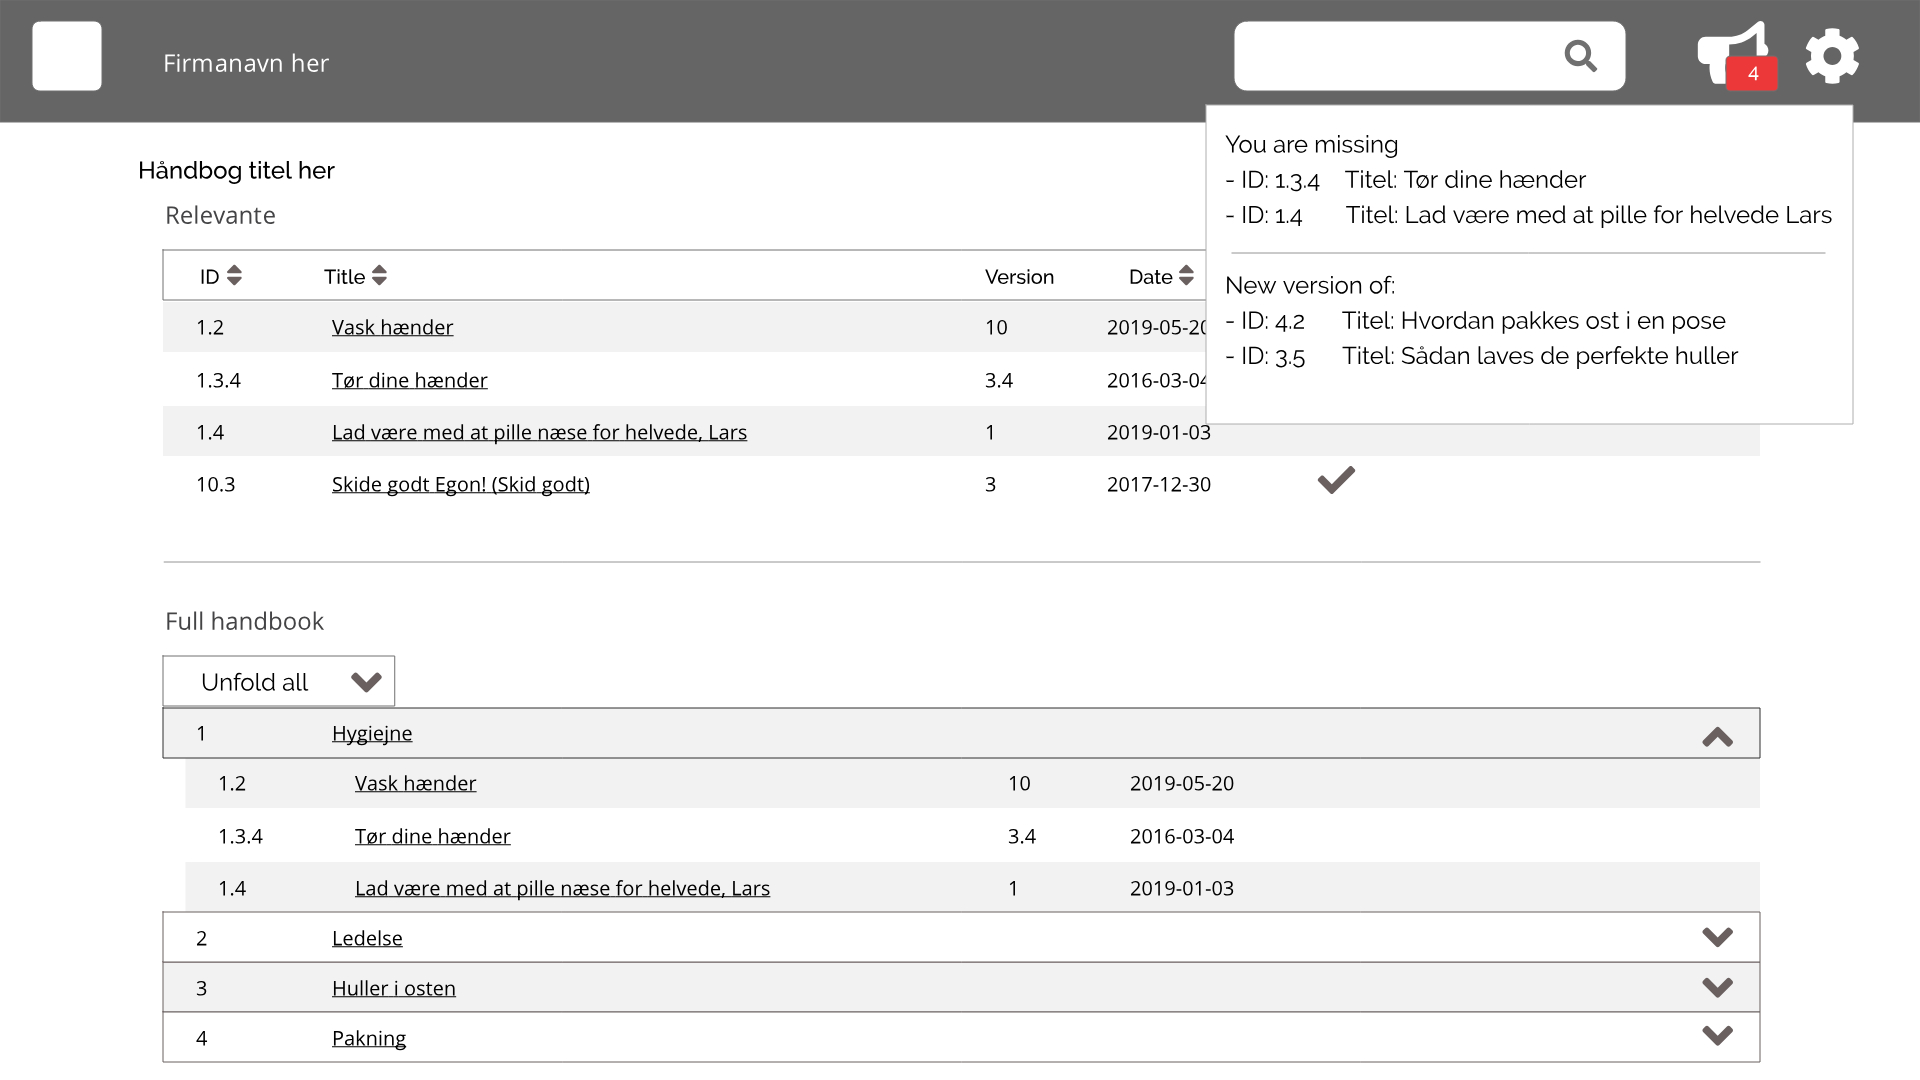
\includegraphics[width=\textwidth]{billeder/iteration2Prototyper/Page_3.jpg}
		\caption{Main interface with notification dropdown}
		\label{fig:4-MainDrop}
	\end{subfigure}
	\quad
	\begin{subfigure}[b]{0.48\textwidth}
		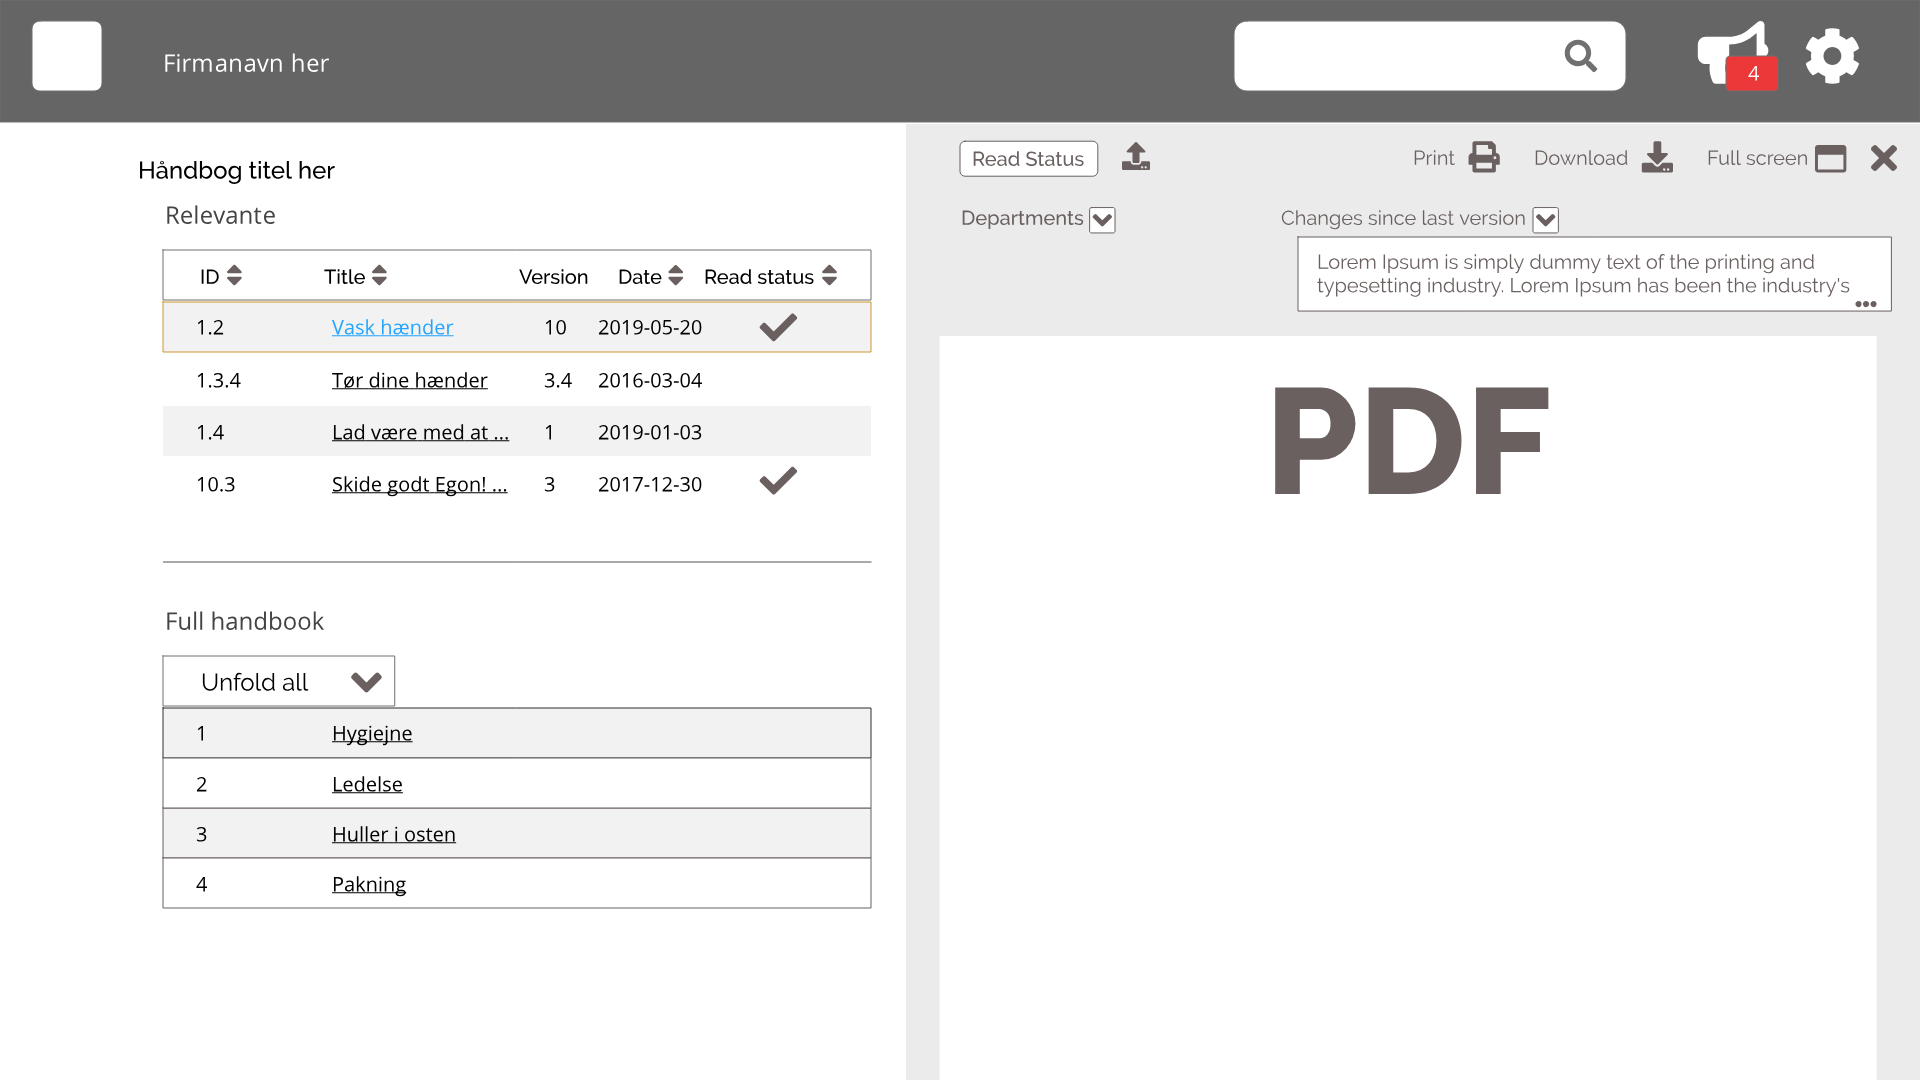
\includegraphics[width=\textwidth]{billeder/iteration2Prototyper/Page_4.jpg}
		\caption{Half document preview}
		\label{fig:4-DocPreviewHalf}
	\end{subfigure}
\end{figure}
\begin{figure}[H]\ContinuedFloat
	\centering
	\begin{subfigure}[b]{0.48\textwidth}
		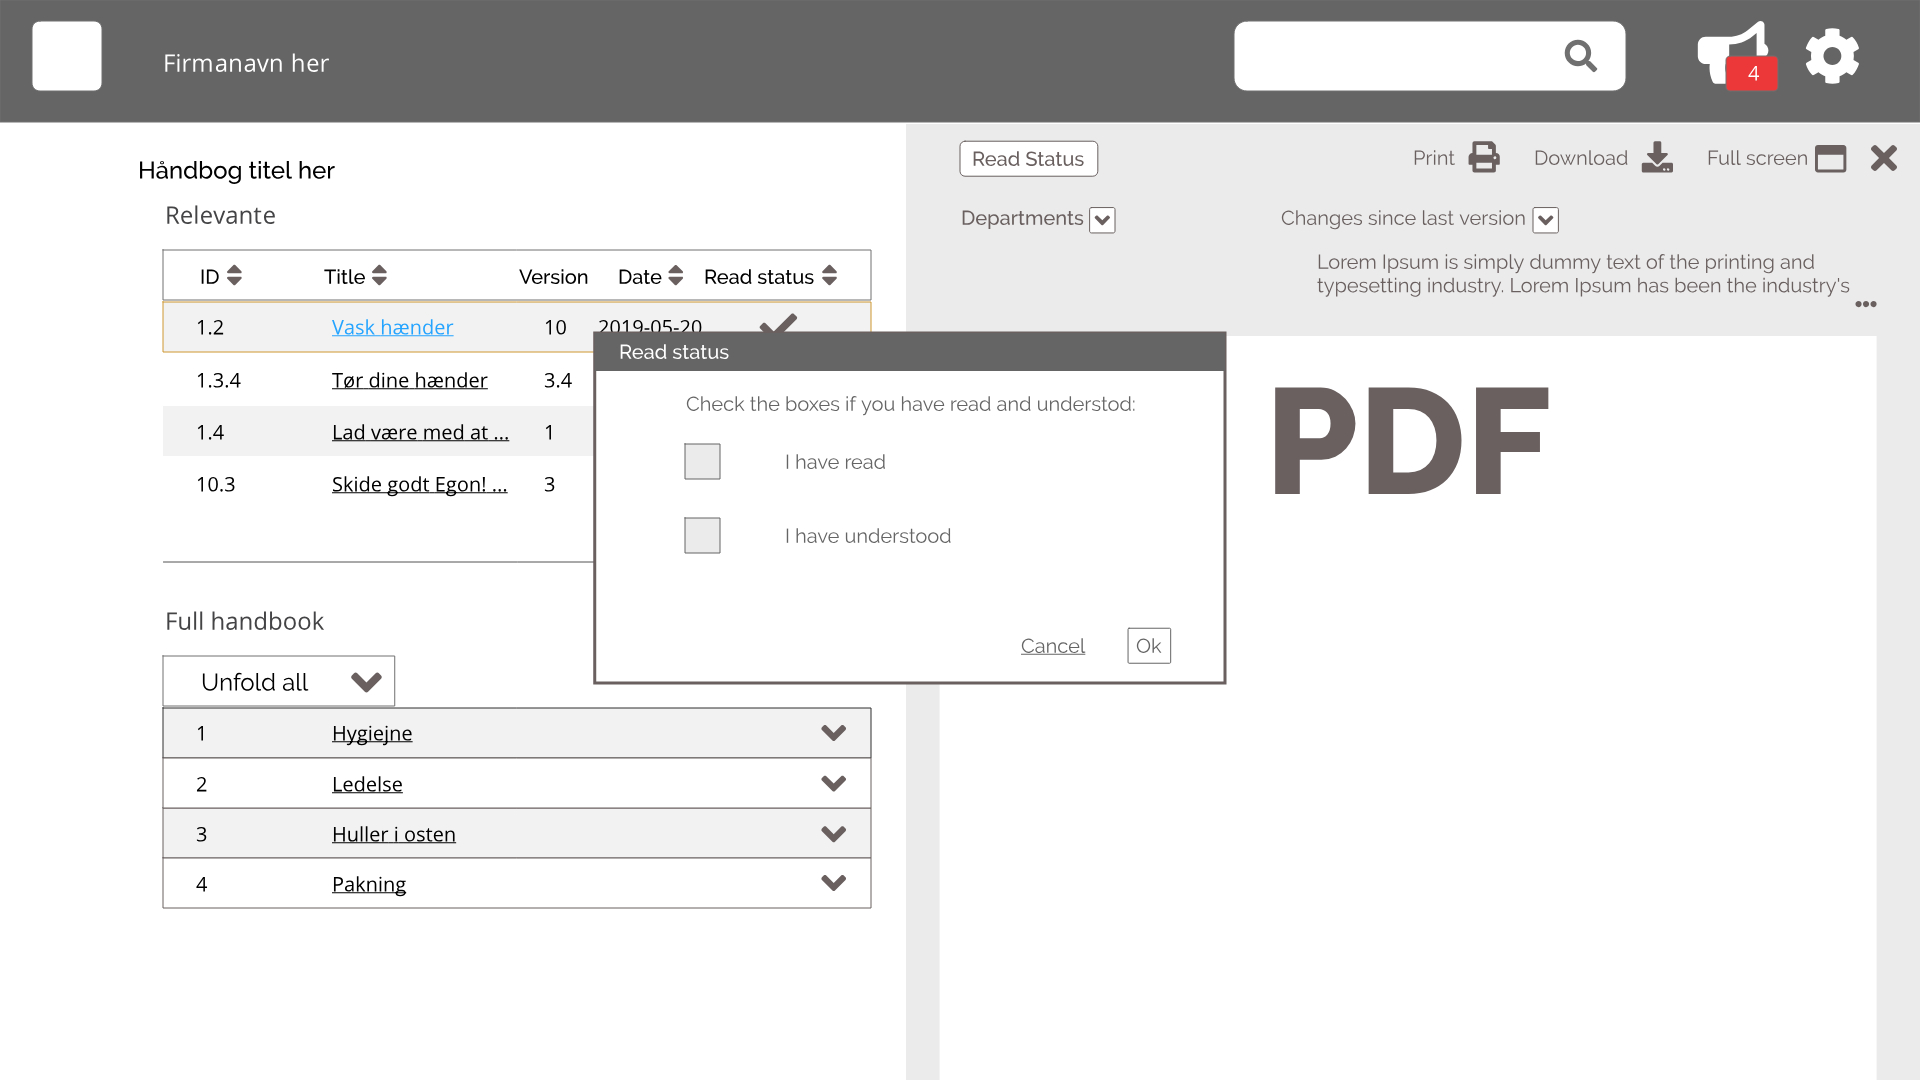
\includegraphics[width=\textwidth]{billeder/iteration2Prototyper/Page_5.jpg}
		\caption{Read status pop-up}
		\label{fig:4-Read}
	\end{subfigure}
	\quad
	\begin{subfigure}[b]{0.48\textwidth}
		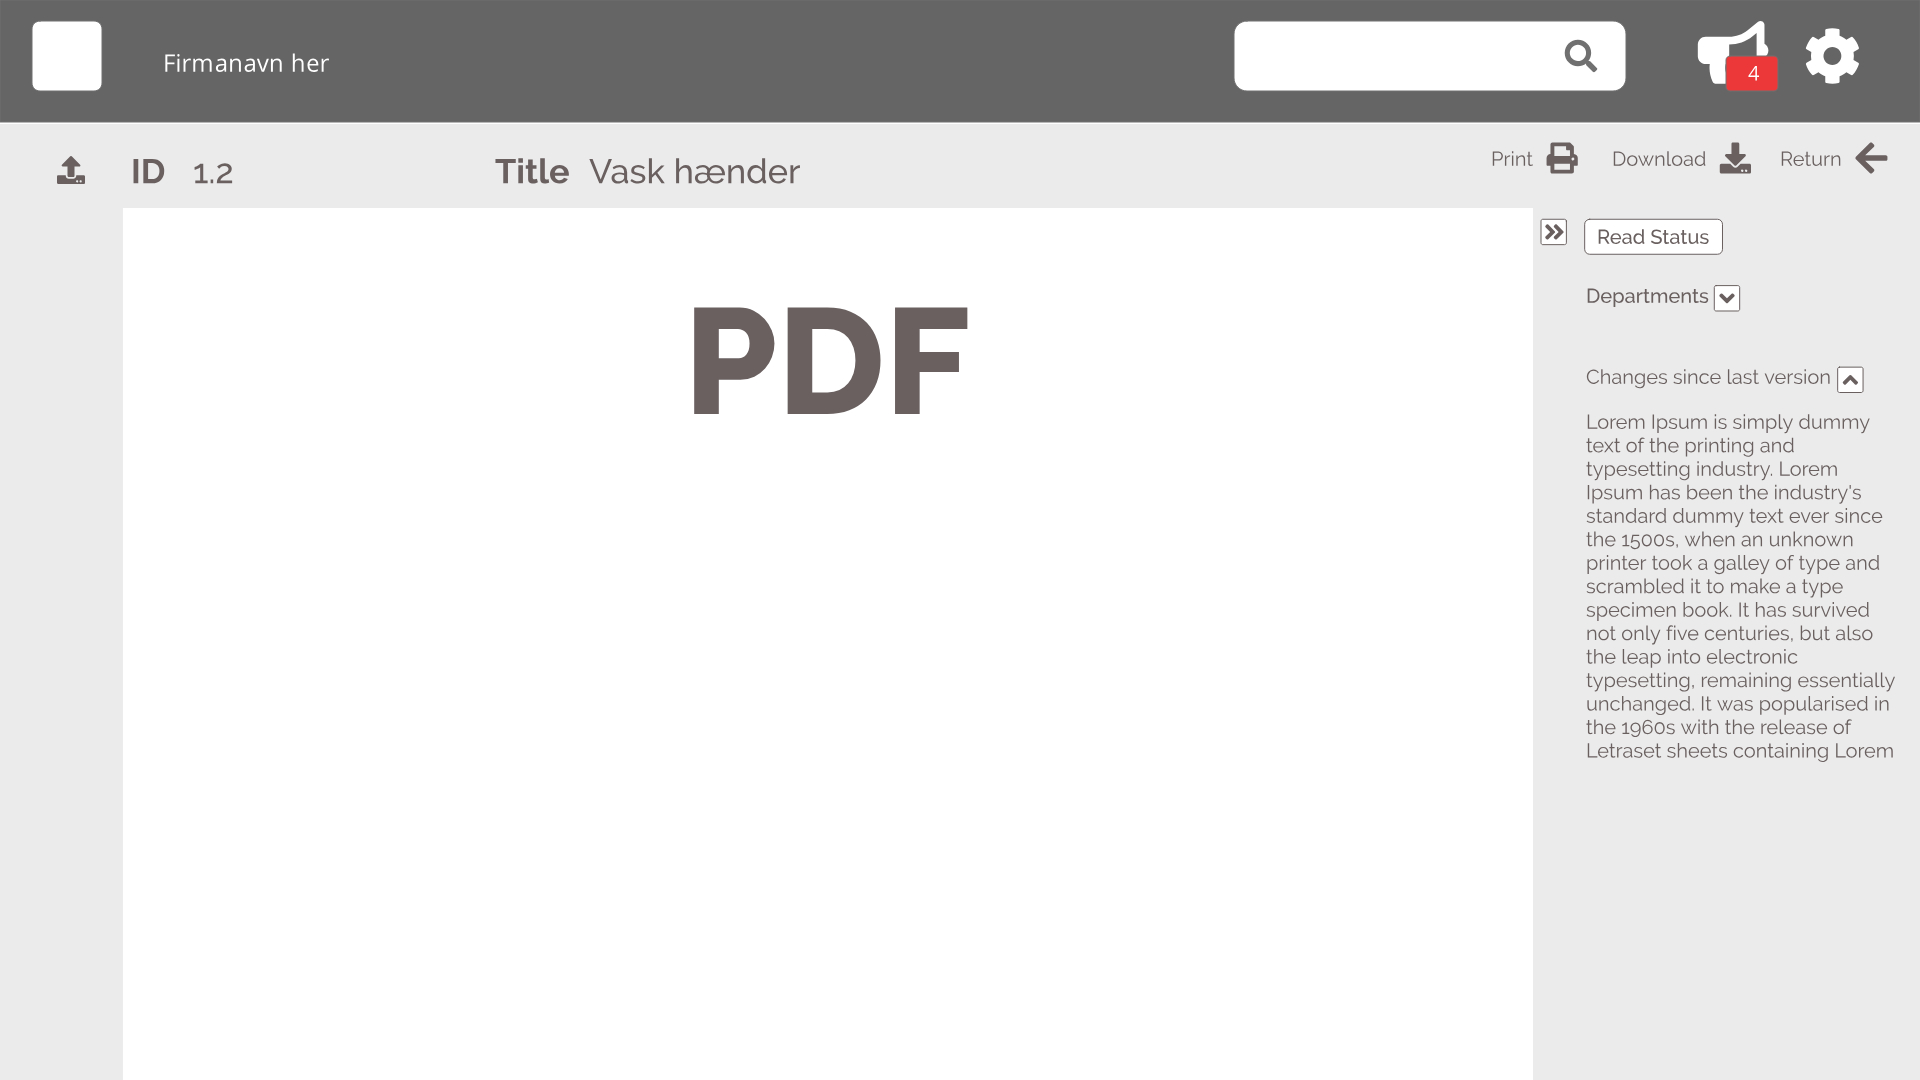
\includegraphics[width=\textwidth]{billeder/iteration2Prototyper/Page_6.jpg}
		\caption{Full document preview}
		\label{fig:4-DocPrevieFull}
	\end{subfigure}
	\caption{Interface design from Mock-up}\label{fig:4-MockUp}
\end{figure}

\section{Main interfaces from prototype for fourth meeting with Ipsen}\label{sec:2prototype}

\chapter{Third Iteration Prototypes} \label{chap:3-Prototypes}
\section{Mockup Continued Development}\label{sec:2Mock}
%Første Blok
\begin{figure}[H]
	\centering
	\begin{subfigure}[b]{0.48\textwidth}
		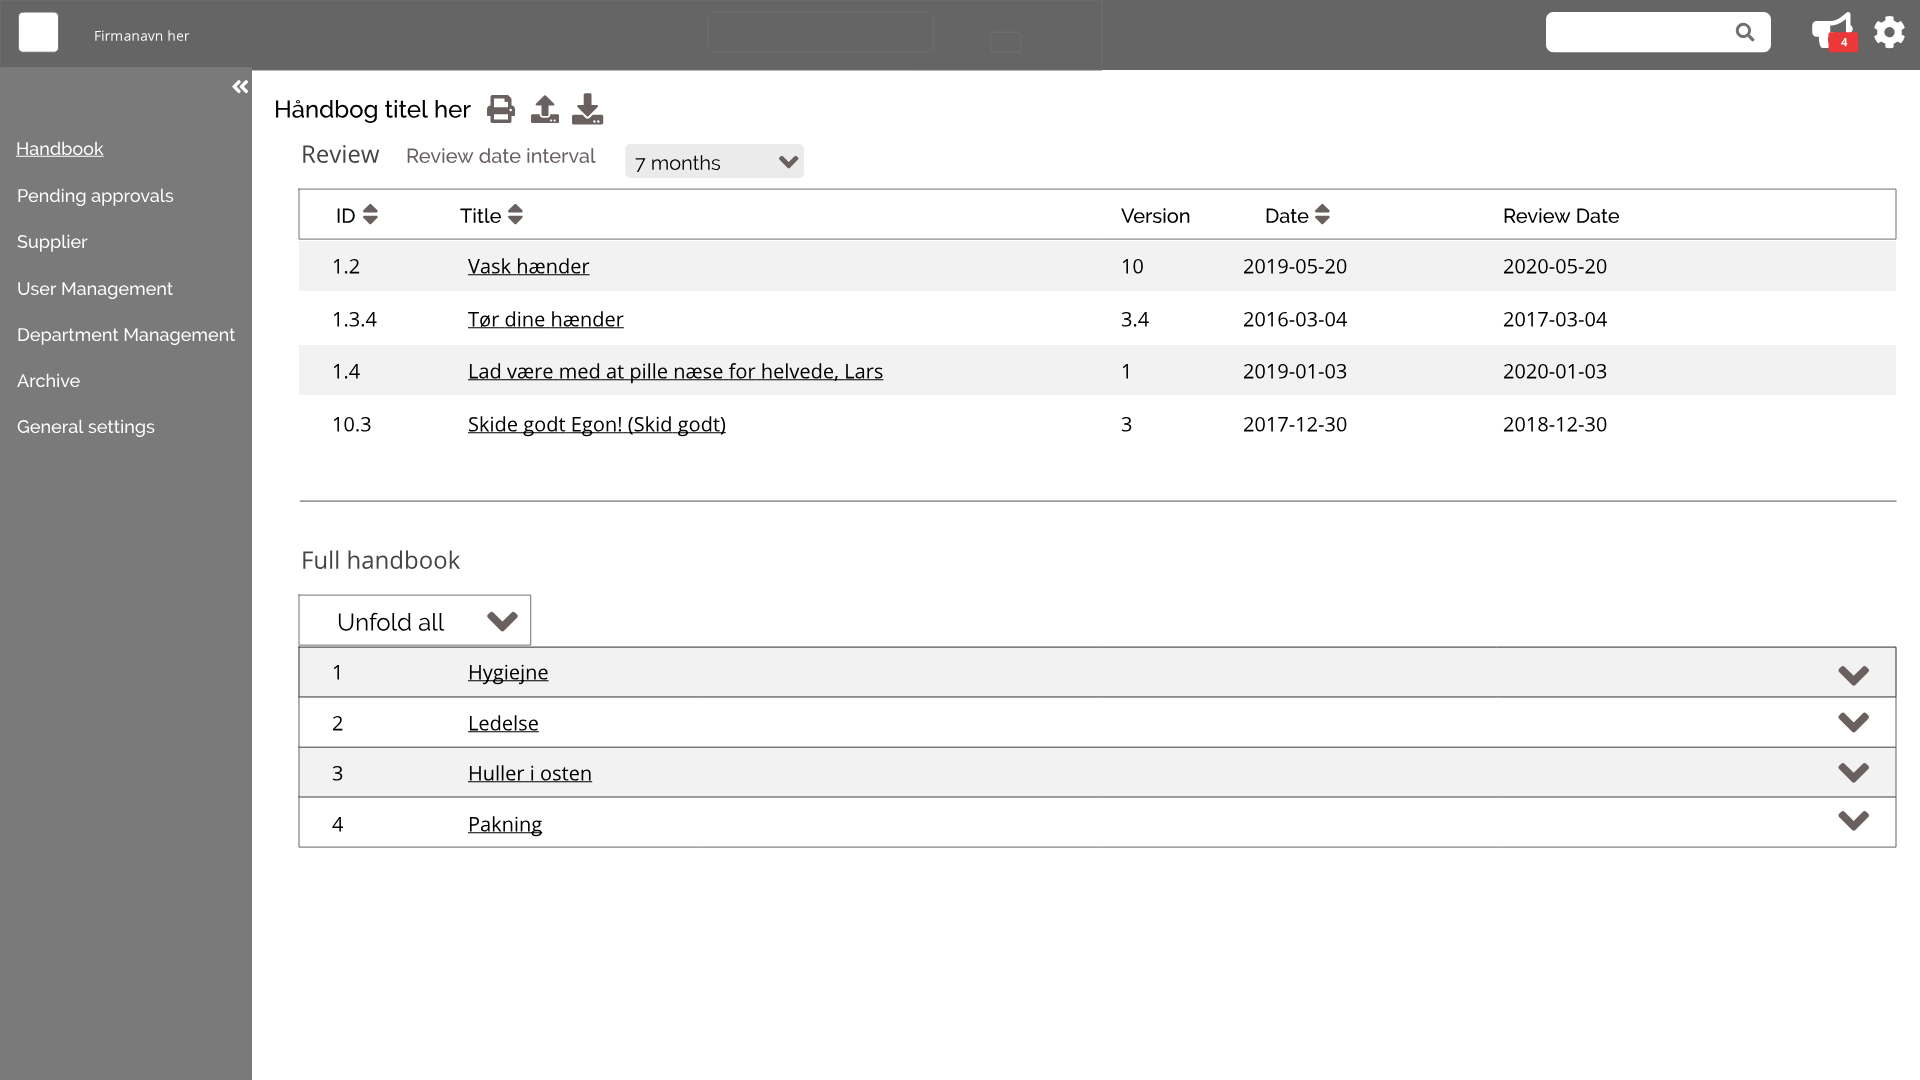
\includegraphics[width=\textwidth]{billeder/iteration3Prototyper/Page_11.jpg}
		\caption{Administrator's main interface 1}
		\label{fig:5-Main1}
	\end{subfigure}
	\quad
	\begin{subfigure}[b]{0.48\textwidth}
		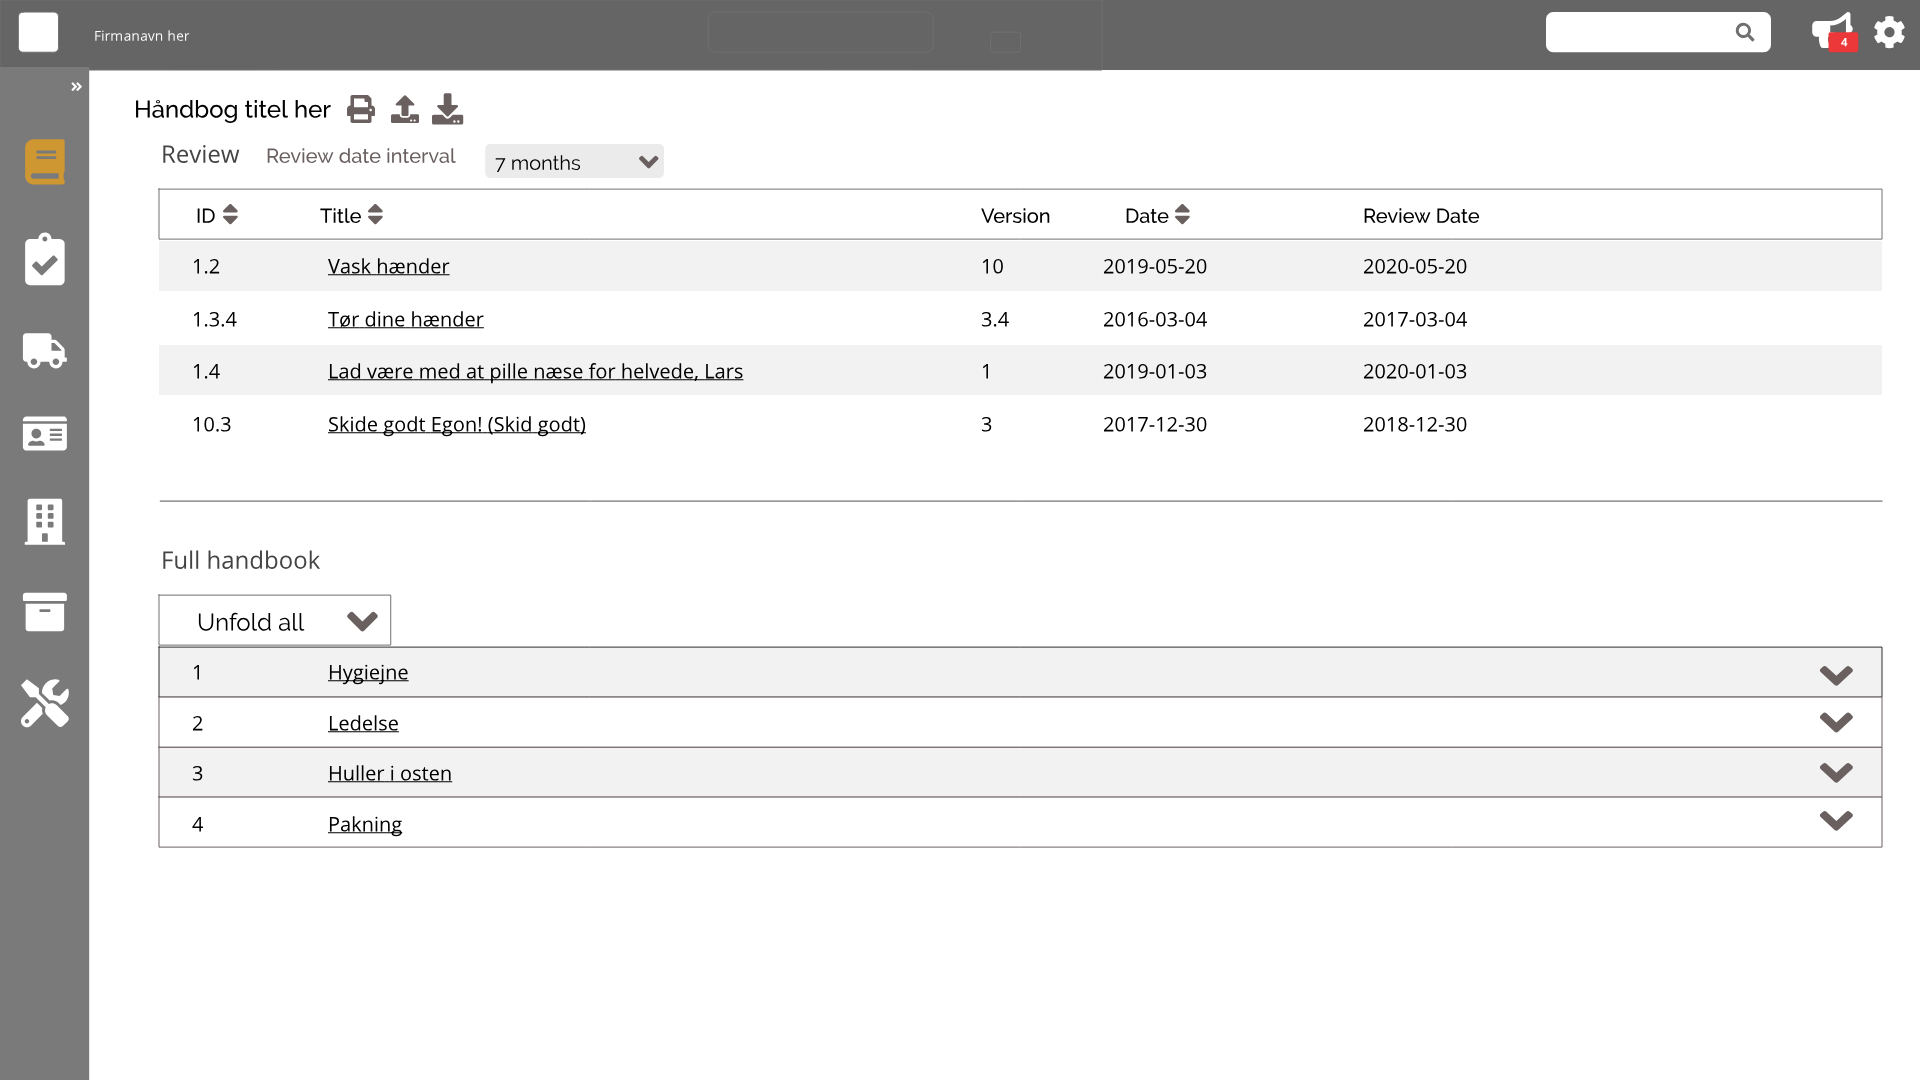
\includegraphics[width=\textwidth]{billeder/iteration3Prototyper/Page_13.jpg}
		\caption{Administrator's main interface 2}
		\label{fig:5-Main2}
	\end{subfigure}
\end{figure}
\begin{figure}[H]\ContinuedFloat
	\centering
	\begin{subfigure}[b]{0.48\textwidth}
		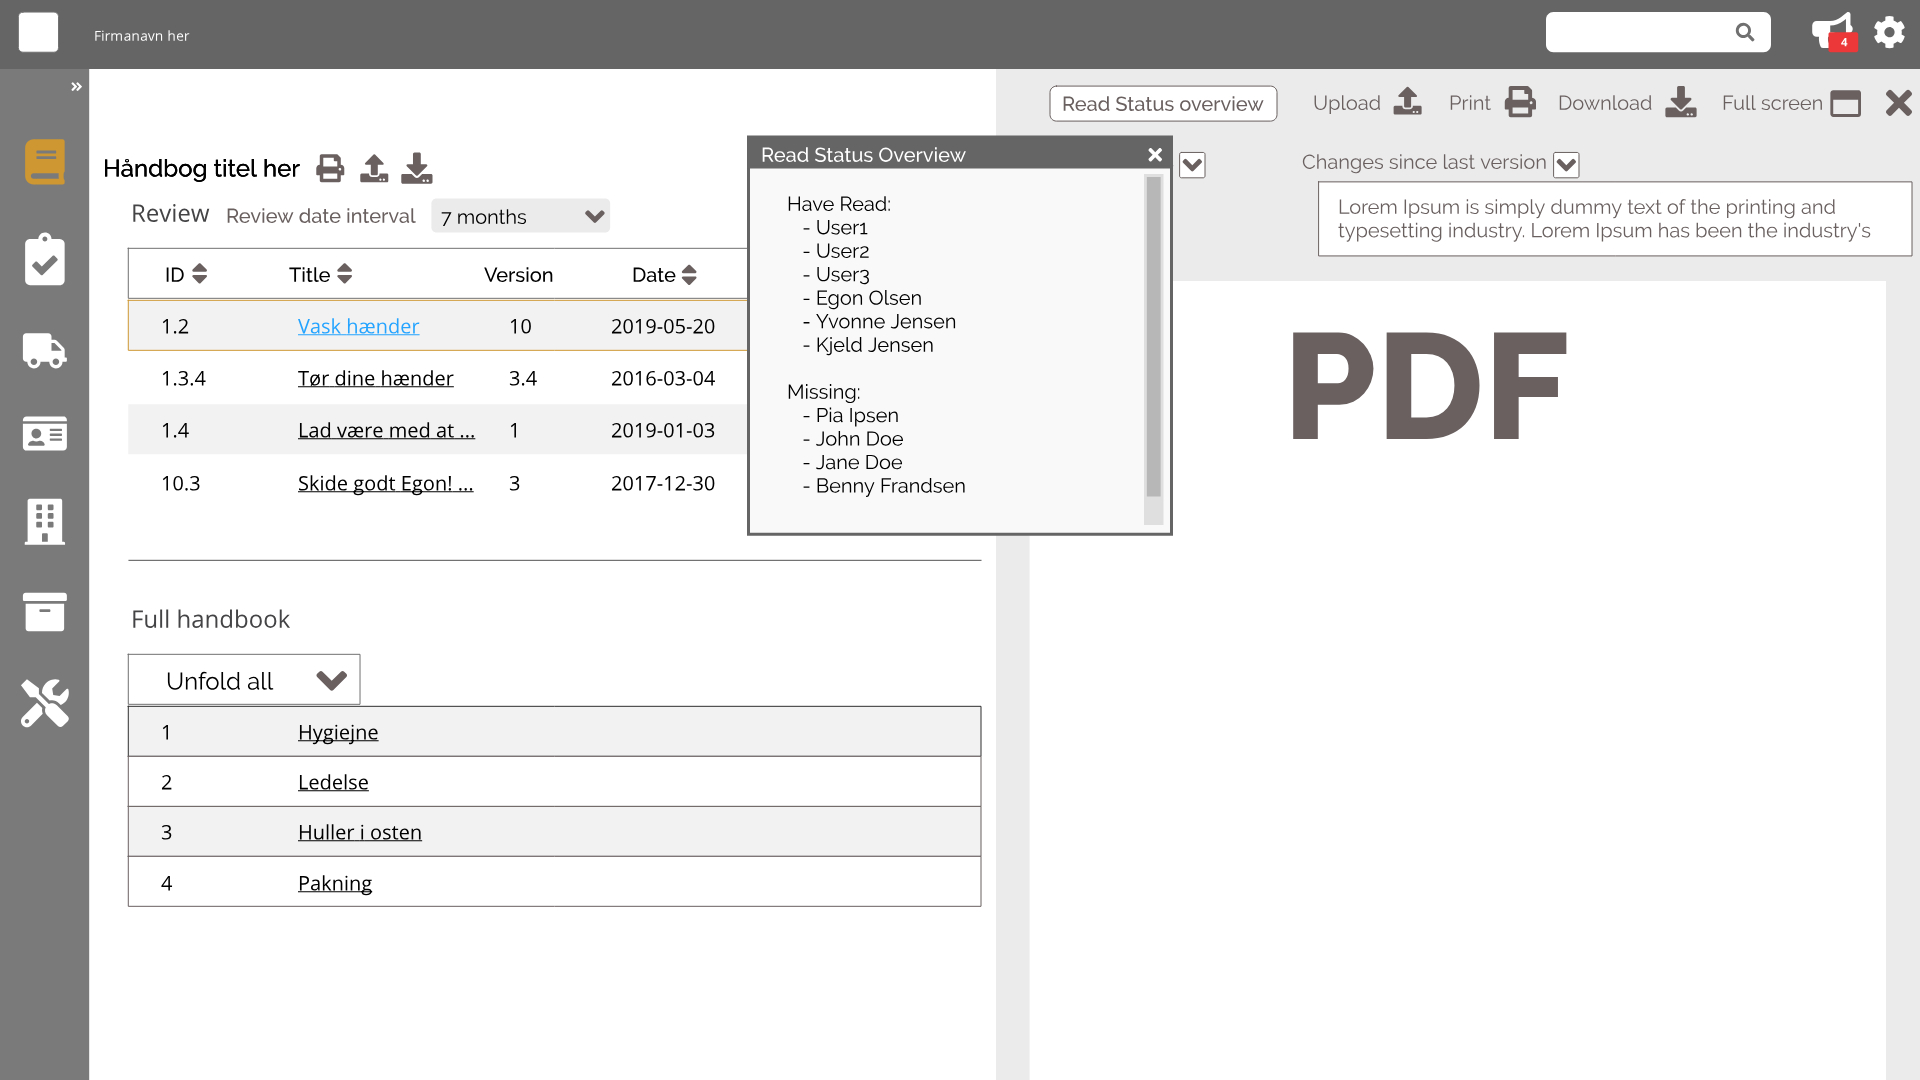
\includegraphics[width=\textwidth]{billeder/iteration3Prototyper/Page_15.jpg}
		\caption{Document preview and read status overview}
		\label{fig:5-PreviewRead}
	\end{subfigure}
	\quad
	\begin{subfigure}[b]{0.48\textwidth}
		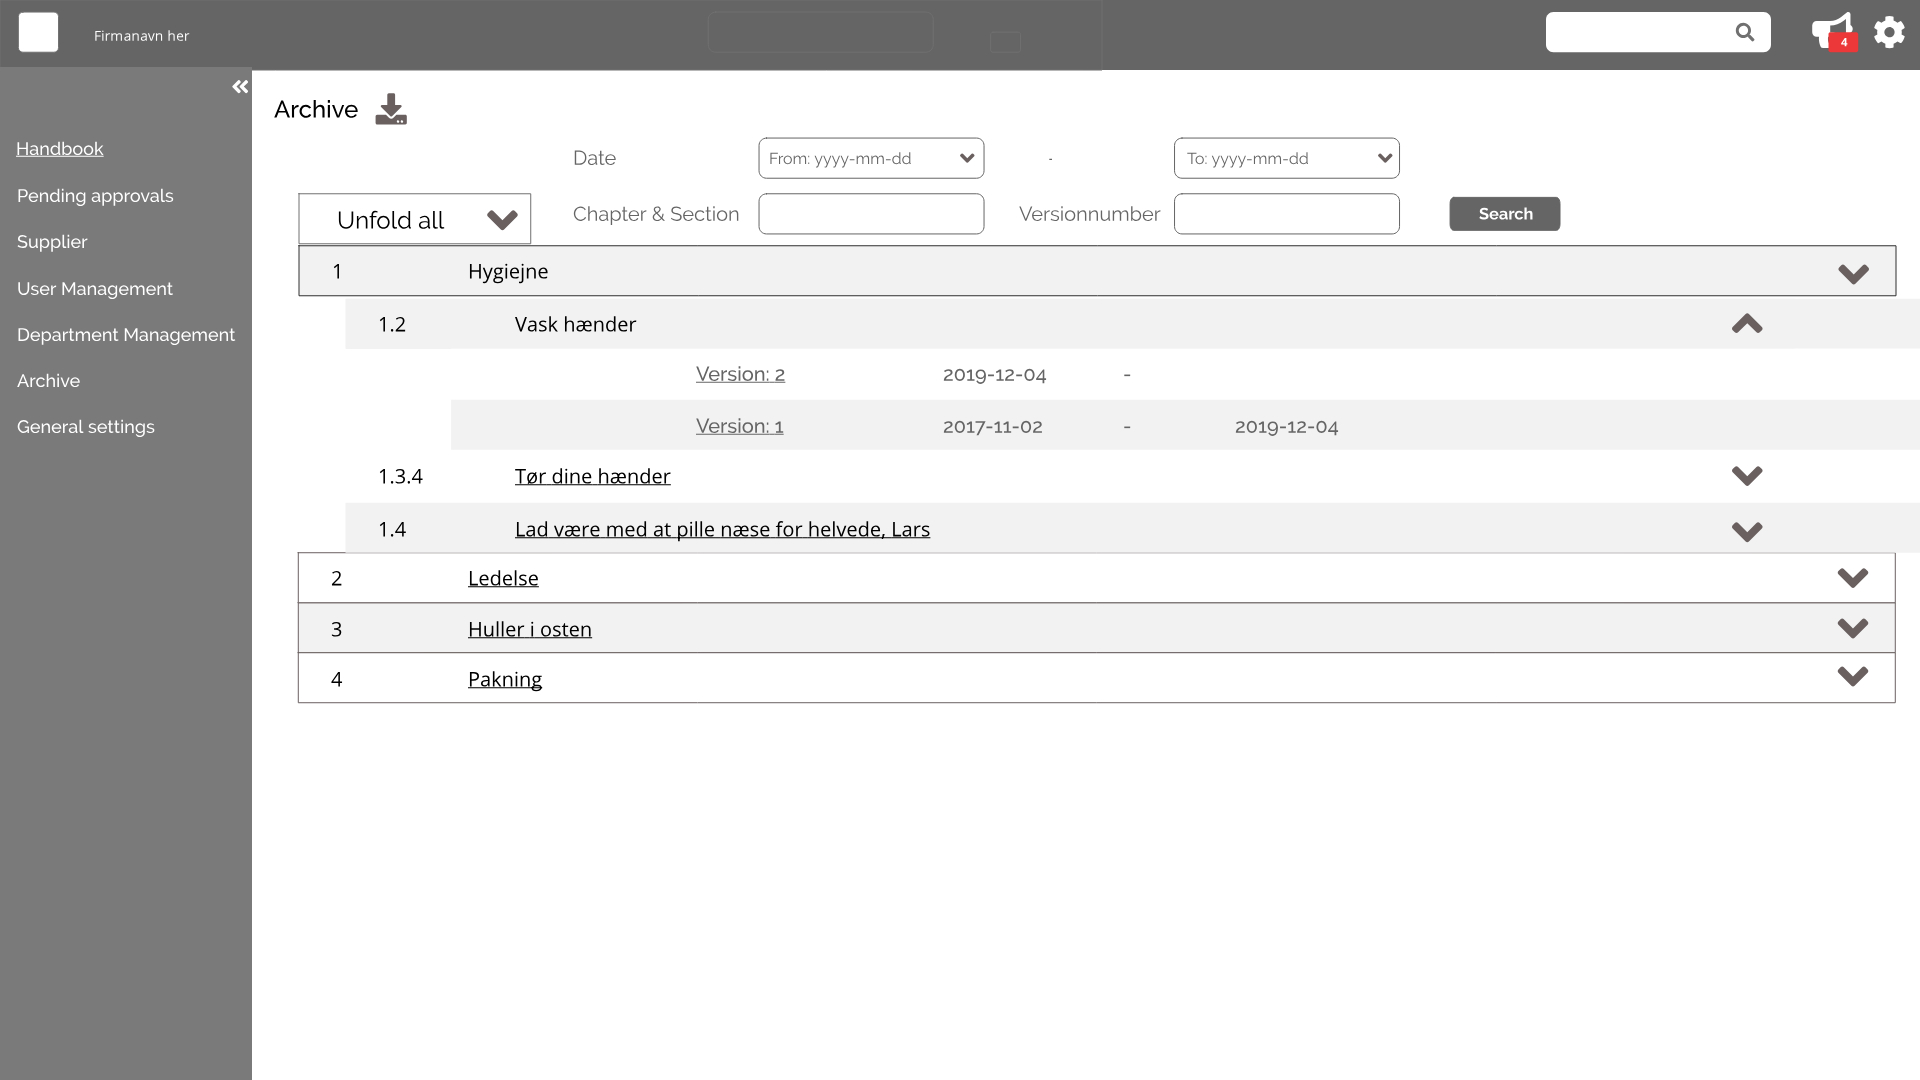
\includegraphics[width=\textwidth]{billeder/iteration3Prototyper/Page_16.jpg}
		\caption{Archive main page}
		\label{fig:5-Archive}
	\end{subfigure}
	\caption{Main and archive interface design from mockup}\label{fig:5-GeneralMockUp}
\end{figure}

%Anden blok
\begin{figure}[H]
	\centering
	\begin{subfigure}[b]{0.48\textwidth}
		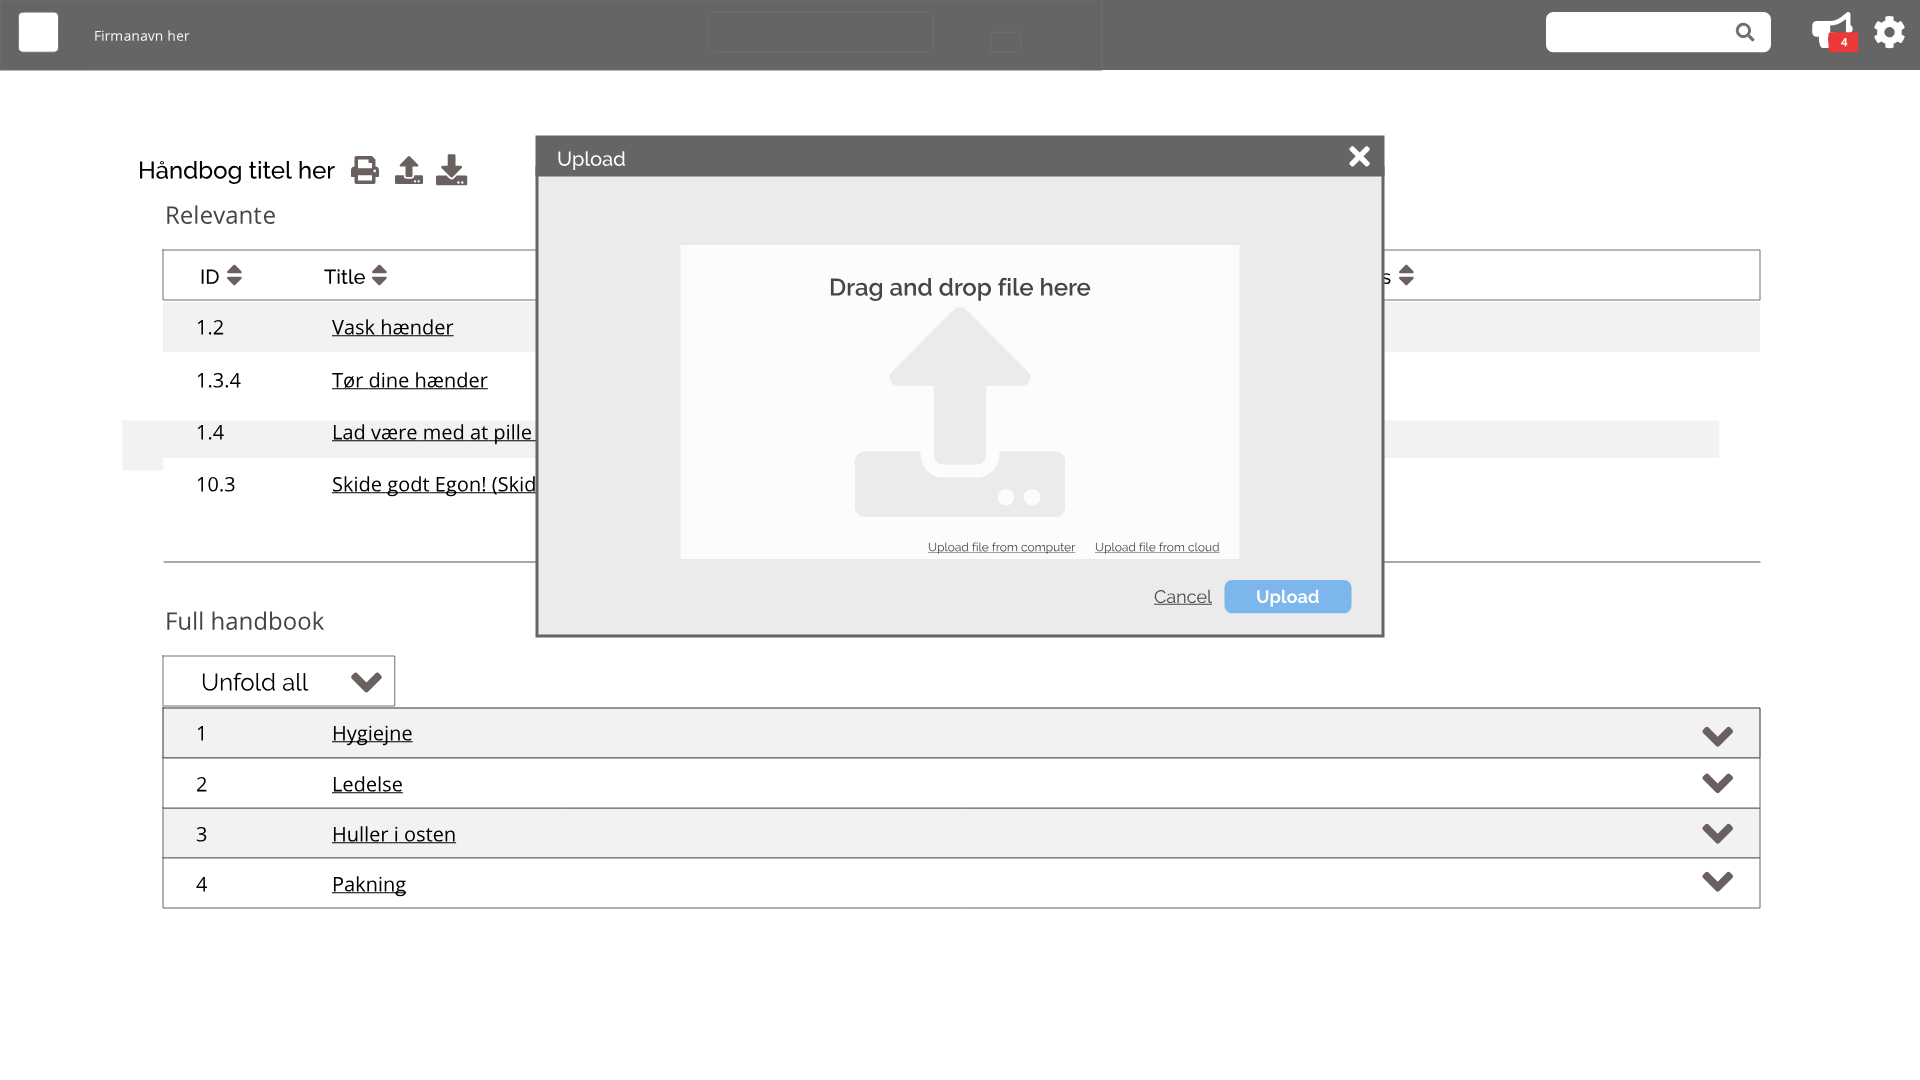
\includegraphics[width=\textwidth]{billeder/iteration3Prototyper/Page_8.jpg}
		\caption{Drag and drop upload}
		\label{fig:5-Upload1}
	\end{subfigure}
	\quad
	\begin{subfigure}[b]{0.48\textwidth}
		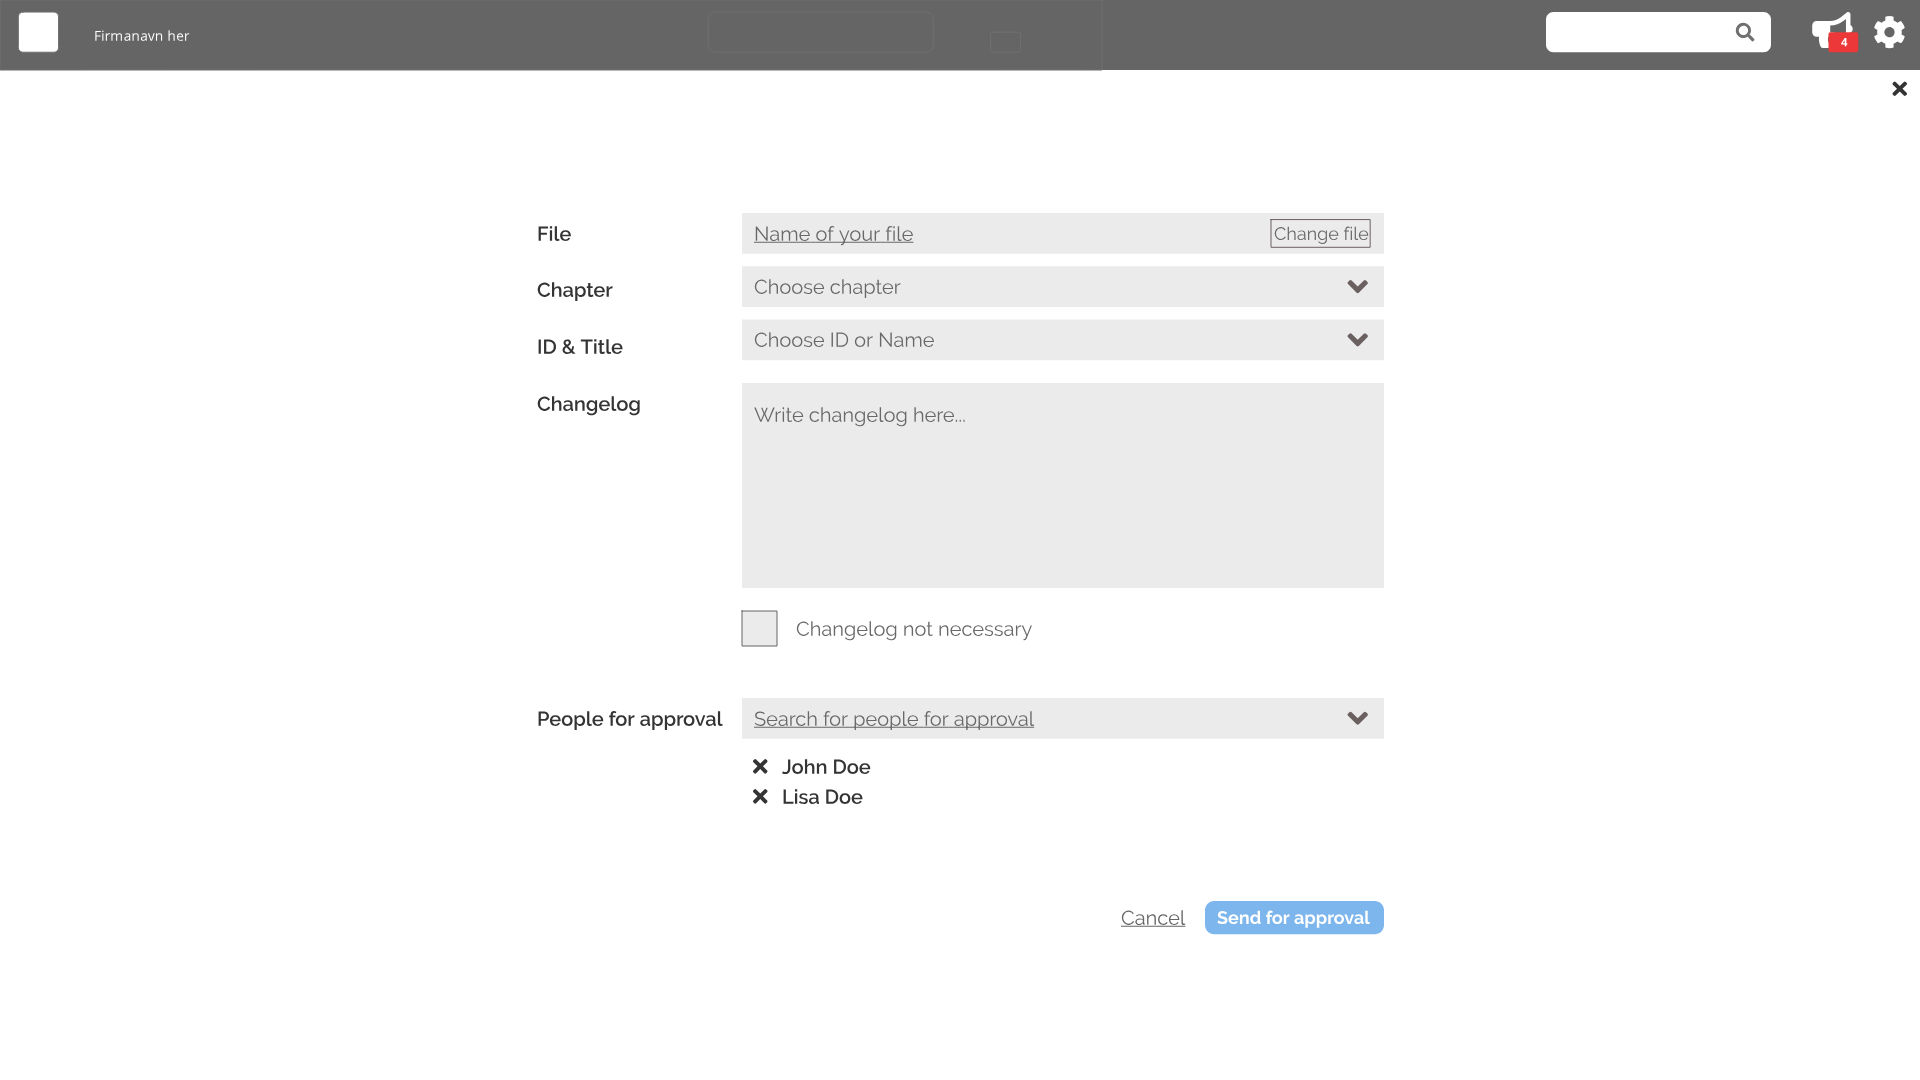
\includegraphics[width=\textwidth]{billeder/iteration3Prototyper/Page_9.jpg}
		\caption{Upload new version or document main interface}
		\label{fig:5-Upload2}
	\end{subfigure}
\end{figure}
\begin{figure}[H]\ContinuedFloat
	\centering
	\begin{subfigure}[b]{0.48\textwidth}
		\includegraphics[width=\textwidth]{billeder/iteration3Prototyper/Page_10.jpg}
		\caption{Upload with dropdowns open}
		\label{fig:5-Upload 3}
	\end{subfigure}
	\quad
	\begin{subfigure}[b]{0.48\textwidth}
		\includegraphics[width=\textwidth]{billeder/iteration3Prototyper/Page_18.jpg}
		\caption{Pending approval main interface}
		\label{fig:5-Approval1}
	\end{subfigure}
\end{figure}
\begin{figure}[H]\ContinuedFloat
	\centering
	\begin{subfigure}[b]{0.48\textwidth}
		\includegraphics[width=\textwidth]{billeder/iteration3Prototyper/Page_19.jpg}
		\caption{Pending approval preview interface}
		\label{fig:5-Approval2}
	\end{subfigure}
	\caption{Upload and approval main interface design from mockup}\label{fig:5-DocMockUp}
\end{figure}

%Tredje blok
\begin{figure}[H]
	\centering
	\begin{subfigure}[b]{0.48\textwidth}
		\includegraphics[width=\textwidth]{billeder/iteration3Prototyper/Page_20.jpg}
		\caption{User management main interface}
		\label{fig:5-UserMan}
	\end{subfigure}
	\quad
	\begin{subfigure}[b]{0.48\textwidth}
		\includegraphics[width=\textwidth]{billeder/iteration3Prototyper/Page_21.jpg}
		\caption{User management edit user interface}
		\label{fig:5-UserManEdit}
	\end{subfigure}
\end{figure}
\begin{figure}[H]\ContinuedFloat
	\centering
	\begin{subfigure}[b]{0.48\textwidth}
		\includegraphics[width=\textwidth]{billeder/iteration3Prototyper/Page_27.jpg}
		\caption{Profile setting main interface}
		\label{fig:5-Profile}
	\end{subfigure}
	\quad
	\begin{subfigure}[b]{0.48\textwidth}
		\includegraphics[width=\textwidth]{billeder/iteration3Prototyper/Page_28.jpg}
		\caption{Edit profile setting interface}
		\label{fig:5-ProfileEdit}
	\end{subfigure}
	\caption{User information interface design from mockup}\label{fig:5-UserMockUp}
\end{figure}


%Fjerde blok
\begin{figure}[H]
	\centering
	\begin{subfigure}[b]{0.48\textwidth}
		\includegraphics[width=\textwidth]{billeder/iteration3Prototyper/Page_22.jpg}
		\caption{Department main interface}
		\label{fig:5-Depart}
	\end{subfigure}
	\quad
	\begin{subfigure}[b]{0.48\textwidth}
		\includegraphics[width=\textwidth]{billeder/iteration3Prototyper/Page_24.jpg}
		\caption{Tried adding existing department interface}
		\label{fig:5-AddDepWrong}
	\end{subfigure}
\end{figure}
\begin{figure}[H]\ContinuedFloat
	\centering
	\begin{subfigure}[b]{0.48\textwidth}
		\includegraphics[width=\textwidth]{billeder/iteration3Prototyper/Page_25.jpg}
		\caption{Department detail interface}
		\label{fig:5-DepDetail}
	\end{subfigure}
	\quad
	\begin{subfigure}[b]{0.48\textwidth}
		\includegraphics[width=\textwidth]{billeder/iteration3Prototyper/Page_26.jpg}
		\caption{Department manage users and documents}
		\label{fig:5-DepEdit}
	\end{subfigure}
	\caption{Department interface design from mockup}\label{fig:5-DepMockUp}
\end{figure}

\newpage
\section{Main Interfaces From Prototype For Fifth Meeting With Ipsen}\label{sec:3prototype}
%Første blpok af billeder
\begin{figure}[H]
	\centering
	\begin{subfigure}[b]{0.48\textwidth}
		\includegraphics[width=\textwidth]{billeder/iteration3Prototyper/MainWriteAdmin.png}
		\caption{First main interface for writer and administrator}
		\label{fig:5-Main1Write}
	\end{subfigure}
	\quad
	\begin{subfigure}[b]{0.48\textwidth}
		\includegraphics[width=\textwidth]{billeder/iteration3Prototyper/MainWriteAdmin2.png}
		\caption{Second main interface for writer and administrator}
		\label{fig:5-Main2write}
	\end{subfigure}
\end{figure}
\begin{figure}[H]\ContinuedFloat
	\centering
	\begin{subfigure}[b]{0.48\textwidth}
		\includegraphics[width=\textwidth]{billeder/iteration3Prototyper/Preview.png}
		\caption{Full preview interface for writer and administrator}
		\label{fig:5-FullPreviewWrite}
	\end{subfigure}
	\quad
	\begin{subfigure}[b]{0.48\textwidth}
		\includegraphics[width=\textwidth]{billeder/iteration3Prototyper/PreviewAdmin.png}
		\caption{Prevew interface with half view for writer and administrator}
		\label{fig:5-HalfPreviewWrite}
	\end{subfigure}
\end{figure}
\begin{figure}[H]\ContinuedFloat
	\centering
	\begin{subfigure}[b]{0.48\textwidth}
		\includegraphics[width=\textwidth]{billeder/iteration3Prototyper/AccessDenied.png}
		\caption{Access denied interface for writer when trying to access unauthenticated pages.}
		\label{fig:5-AccessDenied}
	\end{subfigure}
	\caption{Main interface in common with writer and administrator}\label{fig:5-MainWriteAdmin}
\end{figure}

%Anden blok af billeder
\begin{figure}[H]
	\centering
	\begin{subfigure}[b]{0.48\textwidth}
		\includegraphics[width=\textwidth]{billeder/iteration3Prototyper/MainRead.png}
		\caption{Main interface for reader.}
		\label{fig:5-MainRead}
	\end{subfigure}
	\quad
	\begin{subfigure}[b]{0.48\textwidth}
		\includegraphics[width=\textwidth]{billeder/iteration3Prototyper/PreviewReader.png}
		\caption{Preview of document for reader.}
		\label{fig:5-PreviewReader}
	\end{subfigure}
	\caption{Main interface for reader}\label{fig:5-MainReader}
\end{figure}

%Tredje blok af billeder
\begin{figure}[H]
	\centering
	\begin{subfigure}[b]{0.48\textwidth}
		\includegraphics[width=\textwidth]{billeder/iteration3Prototyper/Archive1.png}
		\caption{Main archive interface.}
		\label{fig:5-Archive1}
	\end{subfigure}
	\quad
	\begin{subfigure}[b]{0.48\textwidth}
		\includegraphics[width=\textwidth]{billeder/iteration3Prototyper/Archive2.png}
		\caption{Detail interface of archive.}
		\label{fig:5-Archive2}
	\end{subfigure}
	\caption{Selected interfaces from archive}\label{fig:5-Archives}
\end{figure}

%Fjerde blok af billeder
\begin{figure}[H]
	\centering
	\begin{subfigure}[b]{0.48\textwidth}
		\includegraphics[width=\textwidth]{billeder/iteration3Prototyper/Ver.png}
		\caption{Add a new version.}
		\label{fig:5-Add}
	\end{subfigure}
	\quad
	\begin{subfigure}[b]{0.48\textwidth}
		\includegraphics[width=\textwidth]{billeder/iteration3Prototyper/Approve.png}
		\caption{Pending approval main interface.}
		\label{fig:5-Approve}
	\end{subfigure}
\end{figure}
\begin{figure}[H]\ContinuedFloat
	\centering
	\begin{subfigure}[b]{0.48\textwidth}
		\includegraphics[width=\textwidth]{billeder/iteration3Prototyper/AppConfirm.png}
		\caption{Confirm approval popup.}
		\label{fig:5-AppConfirm}
	\end{subfigure}
	\caption{Interfaces in connection to adding and approving a new version}\label{fig:5-Approval}
\end{figure}

%Femte blok af billeder
\begin{figure}[H]
	\centering
		\includegraphics[width=0.48\textwidth]{billeder/iteration3Prototyper/Setting.png}
		\caption{Company settings}
		\label{fig:5-setting}
\end{figure}

%Sjette blok af billeder
\begin{figure}[H]
	\centering
	\begin{subfigure}[b]{0.48\textwidth}
		\includegraphics[width=\textwidth]{billeder/iteration3Prototyper/EditU.png}
		\caption{Edit own profile information.}
		\label{fig:5-Add}
	\end{subfigure}
	\quad
	\begin{subfigure}[b]{0.48\textwidth}
		\includegraphics[width=\textwidth]{billeder/iteration3Prototyper/UserMan.png}
		\caption{User management main interface for administrator.}
		\label{fig:5-UManagement}
	\end{subfigure}
\end{figure}
\begin{figure}[H]\ContinuedFloat
	\centering
	\begin{subfigure}[b]{0.48\textwidth}
		\includegraphics[width=\textwidth]{billeder/iteration3Prototyper/EditUAdmin.png}
		\caption{Administrators edit user interface.}
		\label{fig:5-EditUAdmind}
	\end{subfigure}
	\quad
	\begin{subfigure}[b]{0.48\textwidth}
		\includegraphics[width=\textwidth]{billeder/iteration3Prototyper/Dep1.png}
		\caption{Department main interface.}
		\label{fig:5-Dep1}
	\end{subfigure}
\end{figure}
\begin{figure}[H]\ContinuedFloat
	\centering
	\begin{subfigure}[b]{0.48\textwidth}
		\includegraphics[width=\textwidth]{billeder/iteration3Prototyper/Dep2.png}
		\caption{Detail interface of a specific department}
		\label{fig:5-Dep2}
	\end{subfigure}
	 \quad
 	\begin{subfigure}[b]{0.48\textwidth}
 		\includegraphics[width=\textwidth]{billeder/iteration3Prototyper/Dep3.png}
 		\caption{Edit users in department.}
 		\label{fig:5-Dep3}
 	\end{subfigure}
	\caption{Interfaces for department and user information}\label{fig:5-DepEditU}
\end{figure}


\chapter{Usability Testing} \label{bilag:utestbilag}
The methods using to develop the test plan are based on \citep[p.~65-91]{HandbookofUsabilityTesting}. 

\section{Research questions}
The research questions are used to support observations to gain a better understanding of the test subject's point of view regarding the current state of the application. 
However it is not necessarily to be answered.

\begin{itemize}
	\item Are user able to create a document and add a version effortlessly?
	\item Does user understand the Approval functionality in the application?
	\item How well does the flow of the application reflects the expected work flow of user?
	\item How easily and successfully do user navigate through the application? 
	\item What obstacles does user meet when handling common task?
	\item Are the symbols and icons understandable and intuitive? 
	\item What are user impression of the design?
\end{itemize}

\section{Method description}
The usability testing will be perform in stages as described below.

\subsection{Session outline and timing}
The length of the test session is estimated to be one hour. The first 5 minutes will be used to introduce the test subject the usability testing structure and the think aloud principle and 20 minutes in debriefing session. 

\textbf{Introduction to the session}
Test monitor will introduce and explain to test subject how the test going to be conducted, how recording system works and the reason using these and the importance of the thinking aloud method during the test. 

\textbf{Tasks}
Test subject attempts to complete the prepared task list while test monitor observes user interaction with the application. 
Test subject has an option to ask test monitor for clarification if needed however test monitor will not help solving tasks. 

\textbf{Debriefing session}
Post-test questions will be asked to gain a better insight into user's preference and overall experience with the application. 
The debriefing session will also allow discussion to take place if desired. 

\section{Task list (First usability test)}
To be able perform a optimal usability test a task list has been prepared beforehand. 
The test subject will be asked to think aloud while solving the task.
The task list is formulated in in Danish as seen below.
 %The usability testing would be screen recorded and the test subject's interaction with the mouse and the keyboard will be recorded as well. 

Forestil dig at du arbejder som kvalitetschef hos et firma, der producerer boller. 
Du har ansvaret for firmaets håndbog og dens dokumenter. 
I firmaet er der ca. 50 medarbejdere i forskellige afdelinger, som hver især skal læse forskellige dokumenter i håndbogen. 
Det er din opgave at opdatere dokumenterne og sørge for, at de rigtige medarbejdere læser de relevante dokumenter. 
I har netop lanceret en produktion af tranebærboller.

\textbf{Setting:}
Du logger ind på systemet som administrator
På computeren i mappen “Desktop/Håndbøger” ligger “KanLauritzenLevereTranebær.pdf”  og “LauritzenKanLevereTranebær.pdf” af et dokument som skal indføres i håndbogen.

\textbf{Startup:}
\begin{enumerate}
	\item Log ind:
		\begin{itemize}
			\item Email: ips@qmsconsult.dk
			\item Kodeord: K0d30rd   (hvor 0 = nul)
		\end{itemize}

\textbf{Manage documents:}
	\item Tilføj et dokument med titlen “tranebærindkøb”. Placér det i et passende kapitel.
	\item Tilføj første version af dette dokument, “KanLauritzenLevereTranebær.pdf”-
	\item Brug dine administratorrettigheder til selv at godkende første version.
	\item Gå ind og læs dokumentet.
	\item Opdatér dokumentet med en ny version, “LauritzenKanLevereTranebær.pdf”.
	\item Sæt Egon Olsen som godkender af dette dokument og send det til godkendelse.

\textbf{Manage users \& departments:}
	\item Benny Frandsen er blevet ansat. Tilføj ham i systemet.
		\begin{itemize}
			\item Brugernavn: Benny Frandsen
			\item Email: bf@OB.dk
			\item Kodeord: K0d30rd
			\item Rolle: Reader
		\end{itemize}
	\item Tilføj en “Franz Jäger” afdeling.
	\item Tilføj Benny til “Franz Jäger” afdelingen.
	\item Tilføj dokumentet “tranebærindkøb” til “Franz Jäger” afdelingen.

\textbf{Adgang til arkivet:}
	\item I bliver nu auditeret og skal fremvise Jeres dokumentation for tranbeærindkøbene. Find dokumenterne i arkivet.
\end{enumerate}


\end{document} % Slutter dokumentet - obligatorisk
